% Options for packages loaded elsewhere
\PassOptionsToPackage{unicode}{hyperref}
\PassOptionsToPackage{hyphens}{url}
\PassOptionsToPackage{dvipsnames,svgnames*,x11names*}{xcolor}
%
\documentclass[
]{book}
\usepackage{lmodern}
\usepackage{amssymb,amsmath}
\usepackage{ifxetex,ifluatex}
\ifnum 0\ifxetex 1\fi\ifluatex 1\fi=0 % if pdftex
  \usepackage[T1]{fontenc}
  \usepackage[utf8]{inputenc}
  \usepackage{textcomp} % provide euro and other symbols
\else % if luatex or xetex
  \usepackage{unicode-math}
  \defaultfontfeatures{Scale=MatchLowercase}
  \defaultfontfeatures[\rmfamily]{Ligatures=TeX,Scale=1}
\fi
% Use upquote if available, for straight quotes in verbatim environments
\IfFileExists{upquote.sty}{\usepackage{upquote}}{}
\IfFileExists{microtype.sty}{% use microtype if available
  \usepackage[]{microtype}
  \UseMicrotypeSet[protrusion]{basicmath} % disable protrusion for tt fonts
}{}
\makeatletter
\@ifundefined{KOMAClassName}{% if non-KOMA class
  \IfFileExists{parskip.sty}{%
    \usepackage{parskip}
  }{% else
    \setlength{\parindent}{0pt}
    \setlength{\parskip}{6pt plus 2pt minus 1pt}}
}{% if KOMA class
  \KOMAoptions{parskip=half}}
\makeatother
\usepackage{xcolor}
\IfFileExists{xurl.sty}{\usepackage{xurl}}{} % add URL line breaks if available
\IfFileExists{bookmark.sty}{\usepackage{bookmark}}{\usepackage{hyperref}}
\hypersetup{
  pdftitle={Human-Plant Coevolution (HPC) model General exploration and parameter sensitivity analysis},
  colorlinks=true,
  linkcolor=Maroon,
  filecolor=Maroon,
  citecolor=Blue,
  urlcolor=blue,
  pdfcreator={LaTeX via pandoc}}
\urlstyle{same} % disable monospaced font for URLs
\usepackage{longtable,booktabs}
% Correct order of tables after \paragraph or \subparagraph
\usepackage{etoolbox}
\makeatletter
\patchcmd\longtable{\par}{\if@noskipsec\mbox{}\fi\par}{}{}
\makeatother
% Allow footnotes in longtable head/foot
\IfFileExists{footnotehyper.sty}{\usepackage{footnotehyper}}{\usepackage{footnote}}
\makesavenoteenv{longtable}
\usepackage{graphicx}
\makeatletter
\def\maxwidth{\ifdim\Gin@nat@width>\linewidth\linewidth\else\Gin@nat@width\fi}
\def\maxheight{\ifdim\Gin@nat@height>\textheight\textheight\else\Gin@nat@height\fi}
\makeatother
% Scale images if necessary, so that they will not overflow the page
% margins by default, and it is still possible to overwrite the defaults
% using explicit options in \includegraphics[width, height, ...]{}
\setkeys{Gin}{width=\maxwidth,height=\maxheight,keepaspectratio}
% Set default figure placement to htbp
\makeatletter
\def\fps@figure{htbp}
\makeatother
\setlength{\emergencystretch}{3em} % prevent overfull lines
\providecommand{\tightlist}{%
  \setlength{\itemsep}{0pt}\setlength{\parskip}{0pt}}
\setcounter{secnumdepth}{5}
\usepackage{fancyhdr}
\usepackage{placeins}
\usepackage{booktabs}
\usepackage{amsthm}
\makeatletter
\def\thm@space@setup{%
  \thm@preskip=8pt plus 2pt minus 4pt
  \thm@postskip=\thm@preskip
}
\makeatother
\newlength{\cslhangindent}
\setlength{\cslhangindent}{1.5em}
\newenvironment{cslreferences}%
  {\setlength{\parindent}{0pt}%
  \everypar{\setlength{\hangindent}{\cslhangindent}}\ignorespaces}%
  {\par}

\title{Human-Plant Coevolution (HPC) modelGeneral exploration and parameter sensitivity analysis}
\author{}
\date{\vspace{-2.5em}2022-06-27}

\begin{document}
\maketitle

\newcommand{\HRule}{\rule{\linewidth}{0.5mm}}

\pagenumbering{gobble}

%\begin{titlepage}
\begin{center}

\textsc{\LARGE
\strong{H}uman-\strong{P}lant \strong{C}oevolution model} 
\\[1cm]
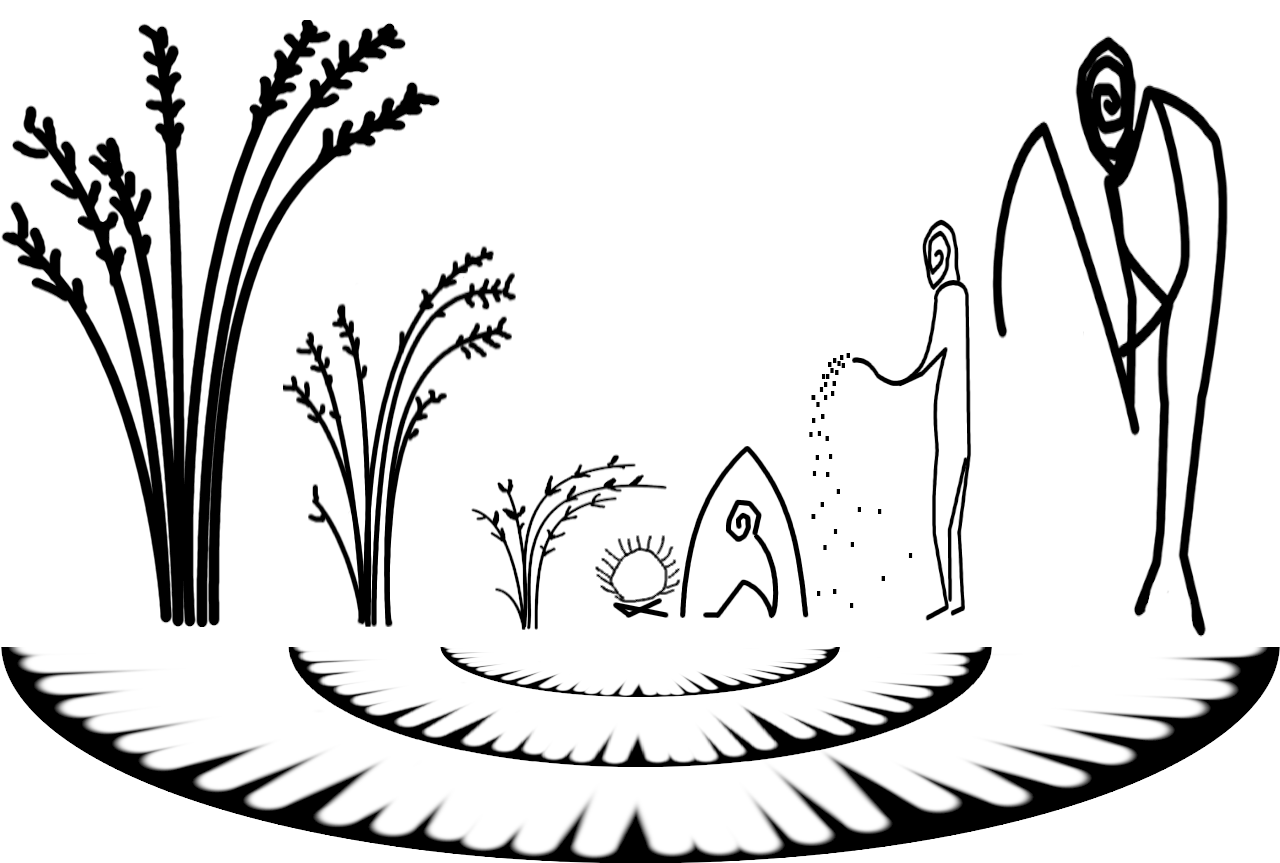
\includegraphics[width=\textwidth]{images/hpcModel-logo_v2.png}
\\[1.5cm]
\HRule \\[0.4cm]
{ \huge General exploration and parameter sensitivity analysis \\[0.15cm] }
\HRule \\[1.5cm]
Andreas Angourakis \& Jon\`{a}s Alcaina
\\[1cm]
\today \\ [1cm]

\end{center}
% \end{titlepage}

\newpage
\pagenumbering{arabic}

{
\hypersetup{linkcolor=}
\setcounter{tocdepth}{1}
\tableofcontents
}
\hypertarget{section}{%
\chapter*{\_\_\_\_\_\_\_}\label{section}}
\addcontentsline{toc}{chapter}{\_\_\_\_\_\_\_}

\hypertarget{model-overview}{%
\chapter*{Model overview}\label{model-overview}}
\addcontentsline{toc}{chapter}{Model overview}

The Human-Plant Coevolution (HPC) model represents the dynamics of coevolution between a human and a plant population. The model consists of an ecological positive feedback system (mutualism), which can be reinforced by positive evolutionary feedback (coevolution). The model is the result of wiring together relatively simple simulation models of population ecology and evolution, through a computational implementation in R.

\newpage

\hypertarget{ecological-relationships-and-population-dynamics}{%
\section*{Ecological relationships and population dynamics}\label{ecological-relationships-and-population-dynamics}}
\addcontentsline{toc}{section}{Ecological relationships and population dynamics}

The model can be expressed by a relatively simple system of two discrete-time difference equations (Eq. 1 and 2), based on the Verhulst-Pearl Logistic equation (chapter 9, Kingsland 1982; Pianka 1974). The change of both populations (\(\Delta H[t]\), \(\Delta P[t]\); see Table 3) depends on an intrinsic growth rate (\(r_{H}, r_{P}\)), the population at a given time (\(H[t]\), \(P[t]\)) and the respective carrying capacity of the environment for each population (\(K_{H}[t]\), \(K_{P}[t]\)), which may vary over time.

\begin{equation}
\tag{Eq. 1}
H[t+1]=H[t]+r_{H}H[t]-r_{H}\frac{H[t]^{2}}{K_{H}[t]}
\end{equation}

\begin{equation}
\tag{Eq. 2}
P[t+1]=P[t]+r_{P}P[t]-r_{P}\frac{P[t]^{2}}{K_{P}[t]}
\end{equation}

Human and plant populations engage in a mutualistic relationship, where one species is to some extent sustained by the other (Eq. 3 and 4). The mutualistic relationship is defined in the model as an increment of the carrying capacity of population B caused by population A (\(U_{AB}[t]\)). This increment, expressed as the utility of A to B at a given time is the product of the utility per capita of A to B (\(\bar{U}_{AB}\)) and the population A at a given time (Eq. 5 and 6).

We consider that both populations are sustained also by an independent term, representing the baseline carrying capacity of the environment or the utility gain from other resources, which is time-dependent (\(U_{bH}[t]\), \(U_{bP}[t]\)). While we assume that the growth of the human population has no predefined ceiling, the expansion of the plant population is considered limited as the area over which plants can grow contiguously (\(MaxArea\)), and represented as a compendium of both space and the maximum energy available in a discrete location (Eq. 4).

\begin{equation}
\tag{Eq. 3}
K_{H}[t]=U_{PH}[t]+U_{bH}[t]
\end{equation}

\begin{equation}
\tag{Eq. 4}
K_{P}[t]=\min(U_{HP}[t]+U_{bP}[t],\, MaxArea)
\end{equation}

\begin{equation}
\tag{Eq. 5}
U_{HP}[t]=H[t]\cdot \bar{U}_{HP}
\end{equation}

\begin{equation}
\tag{Eq. 6}
U_{PH}[t]=P[t]\cdot \bar{U}_{PH}
\end{equation}

Considering that mutualistic relationships involve a positive feedback loop, the population growth at time t improves the conditions for both humans and plants at time \(t + 1\), sustaining their growth even further.

\begin{longtable}[]{@{}ll@{}}
\caption{Assumptions on ecological relationships and population dynamics}\tabularnewline
\toprule
\begin{minipage}[b]{0.45\columnwidth}\raggedright
Domains\strut
\end{minipage} & \begin{minipage}[b]{0.49\columnwidth}\raggedright
Assumptions\strut
\end{minipage}\tabularnewline
\midrule
\endfirsthead
\toprule
\begin{minipage}[b]{0.45\columnwidth}\raggedright
Domains\strut
\end{minipage} & \begin{minipage}[b]{0.49\columnwidth}\raggedright
Assumptions\strut
\end{minipage}\tabularnewline
\midrule
\endhead
\begin{minipage}[t]{0.45\columnwidth}\raggedright
On interacting populations\strut
\end{minipage} & \begin{minipage}[t]{0.49\columnwidth}\raggedright
A population of humans interacts with a population of plants\strut
\end{minipage}\tabularnewline
\begin{minipage}[t]{0.45\columnwidth}\raggedright
On population growth\strut
\end{minipage} & \begin{minipage}[t]{0.49\columnwidth}\raggedright
Population growth is a self-catalyzing process, where the population density in the present will contribute to its own increase in the future, depending on an intrinsic growth rate (\emph{r})\strut
\end{minipage}\tabularnewline
\begin{minipage}[t]{0.45\columnwidth}\raggedright
\strut
\end{minipage} & \begin{minipage}[t]{0.49\columnwidth}\raggedright
Population growth is a self-limiting process, where the population density in the present will constraint its own increase in the future, depending on respective carrying capacity of the environment (\emph{K})\strut
\end{minipage}\tabularnewline
\begin{minipage}[t]{0.45\columnwidth}\raggedright
\strut
\end{minipage} & \begin{minipage}[t]{0.49\columnwidth}\raggedright
The logistic growth model is acceptable as an approximation to the dynamics of populations, both human and plant, under constant conditions\strut
\end{minipage}\tabularnewline
\begin{minipage}[t]{0.45\columnwidth}\raggedright
\strut
\end{minipage} & \begin{minipage}[t]{0.49\columnwidth}\raggedright
The carrying capacity of the environment for a population depends on constant factors and on a time-varying factor (\emph{K{[}t{]}})\strut
\end{minipage}\tabularnewline
\begin{minipage}[t]{0.45\columnwidth}\raggedright
On positive ecological relationships\strut
\end{minipage} & \begin{minipage}[t]{0.49\columnwidth}\raggedright
Positive ecological relationships exist, where an individual of one population increases by an amount the carrying capacity of the environment for another population\strut
\end{minipage}\tabularnewline
\begin{minipage}[t]{0.45\columnwidth}\raggedright
\strut
\end{minipage} & \begin{minipage}[t]{0.49\columnwidth}\raggedright
Coupled positive ecological relationships (i.e., mutualism) exist, where two populations increase the carrying capacities for each other\strut
\end{minipage}\tabularnewline
\begin{minipage}[t]{0.45\columnwidth}\raggedright
\strut
\end{minipage} & \begin{minipage}[t]{0.49\columnwidth}\raggedright
There is variation in positive ecological relationships, so individuals of one population vary in terms of how much they increase the carrying capacity for the other population\strut
\end{minipage}\tabularnewline
\begin{minipage}[t]{0.45\columnwidth}\raggedright
On human-plant mutualism\strut
\end{minipage} & \begin{minipage}[t]{0.49\columnwidth}\raggedright
A given plant species yield a positive utility for humans, e.g., as a source of food and raw materials\strut
\end{minipage}\tabularnewline
\begin{minipage}[t]{0.45\columnwidth}\raggedright
\strut
\end{minipage} & \begin{minipage}[t]{0.49\columnwidth}\raggedright
Humans return a positive utility for this plant species, e.g., by improving soil conditions\strut
\end{minipage}\tabularnewline
\begin{minipage}[t]{0.45\columnwidth}\raggedright
\strut
\end{minipage} & \begin{minipage}[t]{0.49\columnwidth}\raggedright
The utility given by one population adds value to the carrying capacity for the other, and vice versa\strut
\end{minipage}\tabularnewline
\begin{minipage}[t]{0.45\columnwidth}\raggedright
\strut
\end{minipage} & \begin{minipage}[t]{0.49\columnwidth}\raggedright
The carrying capacity for humans rely also in other resources, which are independent of the plant species (i.e., the baseline carrying capacity for humans)\strut
\end{minipage}\tabularnewline
\begin{minipage}[t]{0.45\columnwidth}\raggedright
\strut
\end{minipage} & \begin{minipage}[t]{0.49\columnwidth}\raggedright
The carrying capacity for plants rely also in other conditions, which are independent of humans (i.e., the baseline carrying capacity for plants)\strut
\end{minipage}\tabularnewline
\begin{minipage}[t]{0.45\columnwidth}\raggedright
\strut
\end{minipage} & \begin{minipage}[t]{0.49\columnwidth}\raggedright
The carrying capacity for plants is eventually constrained by the space available for it to grow contiguously as a population (i.e., maximum area)\strut
\end{minipage}\tabularnewline
\bottomrule
\end{longtable}

\newpage

\hypertarget{population-diversity}{%
\section*{Population diversity}\label{population-diversity}}
\addcontentsline{toc}{section}{Population diversity}

The HPC model contemplates a vector (pop) of length n, containing the population fractions of each type. The number of types are population-specific and are given as two parameters (\(n_{H}\), \(n_{P}\)). These types include all possible variations within a population so that this vector amounts to the unity (\(\sum_{i=1}^{n}{pop_{A_{i}}}=1\)).

To account for multiple types, we replace Eq. 5 and 6 with Eq. 7 and 8, where the utility of population A to B at any given time (\(U_{AB}[t]\)) is calculated by summing up the utility per capita of each type (\(\bar{U}_{A_{i}B}\)) proportionally to the share of population of the respective type (\(pop_{A_{i}}[t]\)), and multiplying the result by the population at a given time. The baseline carrying capacity (\(U_{bA_{i}}[t]\)) is calculated in a similar manner, though using the utility that each type is able to gain from other resources (\(U_{bA_{i}}\)) (Eq. 9 and 10).

\begin{equation}
\tag{Eq. 7}
U_{HP}[t]=H[t]\sum_{i=1}^{n_{H}}{pop_{H_{i}}[t]\cdot \bar{U}_{H_{i}P}}
\end{equation}

\begin{equation}
\tag{Eq. 8}
U_{PH}[t]=P[t]\sum_{i=1}^{n_{P}}{pop_{P_{i}}[t]\cdot \bar{U}_{P_{i}H}}
\end{equation}

\begin{equation}
\tag{Eq. 9}
U_{bH}[t]=\sum_{i=1}^{n_{H}}{pop_{H_{i}}[t]\cdot U_{bH_{i}}}
\end{equation}

\begin{equation}
\tag{Eq. 10}
U_{bP}[t]=\sum_{i=1}^{n_{P}}{pop_{P_{i}}[t]\cdot U_{bP_{i}}}
\end{equation}

Types relate to population-specific values of utility per capita (\(\bar{U}_{A_{i}B}\)) and baseline carrying capacity (\(U_{bA_{i}}\)). These values are defined by linear interpolation between pairs of parameters representing the values corresponding to types \(1\) and \(n\) (e.g., if \(n_P=10\), \(\bar{U}_{P_{1}H}=1\) and \(\bar{U}_{P_{n}H}=10\), then \(\bar{U}_{P_{5}H}=5\)). The shares of population within types follow a one-tail distribution rather than a normal distribution, which would be more adequate but less straightforward to use in a theoretical model. Under this circumstance, the distribution of population within types will always be biased towards the intermediate types.

\hypertarget{coevolutionary-dynamics}{%
\section*{Coevolutionary dynamics}\label{coevolutionary-dynamics}}
\addcontentsline{toc}{section}{Coevolutionary dynamics}

Undirected variation, which causes part of the population to randomly change to other types, represents the effect of mutation in genetic transmission or of innovation, error, and other mechanisms in cultural transmission. The balance of the subpopulation A of type \(i\) depends on the level of undirected variation (\(v_{A}\)) and on the degree and sign of the difference between the current subpopulation (\(pop_{A_{i}}[t]\)) and the averaged subpopulation (\(1/n_{A}\)), which refers to the completely uniform distribution among types (Eq. 11 and 12).

\begin{equation}
\tag{Eq. 11}
pop_{H}[t]'=pop_{H}[t]+v_{H}\left(\tfrac{1}{n_{H}}-pop_{H}[t]\right)
\end{equation}

\begin{equation}
\tag{Eq. 12}
pop_{P}[t]'=pop_{P}[t]+v_{P}\left(\tfrac{1}{n_{P}}-pop_{P}[t]\right)
\end{equation}

By considering inertia, we are assuming that the more frequent a type is, the more likely that it is transmitted. Selection is implemented by assigning a fitness score to each type (\(fitness_{A_{i}}[t]\)), which in turn biases its transmission. Equations 13 and 14 summarizes the combined effect that inertia and selection have on the proportion of population A belonging to type \(i\) (\(pop_{A_{i}}[t]\)) {[}for a formal similarity of the discrete replicator dynamic and Bayesian inference see Harper2009{]}.

\begin{equation}
\tag{Eq. 13}
pop_{H_{i}}[t+1]=\frac{fitness_{H_{i}}[t]\cdot pop_{H_{i}}[t]}{\sum_{j=1}^{n_{H}}fitness_{H_{j}}[t]\cdot pop_{H_{j}}[t]}
\end{equation}

\begin{equation}
\tag{Eq. 14}
pop_{P_{i}}[t+1]=\frac{fitness_{P_{i}}[t]\cdot pop_{P_{i}}[t]}{\sum_{j=1}^{n_{P}}fitness_{P_{j}}[t]\cdot pop_{P_{j}}[t]}
\end{equation}

This mechanism defines how a trait evolves in a single population. However, coevolution can also be represented when the selective pressure on this population is modified by the changing traits of another population. In order to link the two populations, fitness scores of population A are derived from the weight of the contribution or utility of population B (\(U_{BA}[t]\)) in relation to the base carrying capacity of A (\(K_{A}[t]\)) (Eq. 10).

\begin{equation}
\tag{Eq. 15}
fitness_{H_{i}}[t]=\frac{(n_{H}-i)\,U_{bH}[t]+i\,U_{PH}[t]}{U_{bH}[t]+U_{PH}[t]}
\end{equation}

\begin{equation}
\tag{Eq. 16}
fitness_{P_{i}}[t]=\frac{(n_{P}-i)\,U_{bP}[t]+i\,U_{HP}[t]}{U_{bP}[t]+U_{HP}[t]}
\end{equation}

As a consequence of this model design, types of both human and plant populations span from a non-mutualistic type (\(i=1\)), which has the best fitness score when there is no positive interaction with the other population (\(U_{BA}[t]\approx 0\)), to a mutualistic type (\(i=n\)), which is the optimum when nearly the whole of the carrying capacity is due to such relationship (\(U_{BA}[t]\approx K_{A}[t]\)).

\begin{longtable}[]{@{}ll@{}}
\caption{Assumptions on population diversity and coevolution}\tabularnewline
\toprule
\begin{minipage}[b]{0.45\columnwidth}\raggedright
Domains\strut
\end{minipage} & \begin{minipage}[b]{0.49\columnwidth}\raggedright
Assumptions\strut
\end{minipage}\tabularnewline
\midrule
\endfirsthead
\toprule
\begin{minipage}[b]{0.45\columnwidth}\raggedright
Domains\strut
\end{minipage} & \begin{minipage}[b]{0.49\columnwidth}\raggedright
Assumptions\strut
\end{minipage}\tabularnewline
\midrule
\endhead
\begin{minipage}[t]{0.45\columnwidth}\raggedright
On the evolution of traits\strut
\end{minipage} & \begin{minipage}[t]{0.49\columnwidth}\raggedright
A population can be divided into types according to one or more traitsThe distribution of individuals among types can vary in time, due to factors affecting trait transmission\strut
\end{minipage}\tabularnewline
\begin{minipage}[t]{0.45\columnwidth}\raggedright
On the factors affecting the evolution of traits\strut
\end{minipage} & \begin{minipage}[t]{0.49\columnwidth}\raggedright
Change of the population distribution among types depends on the previous population distribution: the more frequent is a type, the more likely it will be imitated or transmitted to the next generation\strut
\end{minipage}\tabularnewline
\begin{minipage}[t]{0.45\columnwidth}\raggedright
\strut
\end{minipage} & \begin{minipage}[t]{0.49\columnwidth}\raggedright
Change of the population distribution among types depends on the relative fitness of types: the greater the fitness score associated to a type, the more likely it will be imitated or transmitted to the next generation\strut
\end{minipage}\tabularnewline
\begin{minipage}[t]{0.45\columnwidth}\raggedright
\strut
\end{minipage} & \begin{minipage}[t]{0.49\columnwidth}\raggedright
Change of the population distribution among types depends on undirected variation\strut
\end{minipage}\tabularnewline
\begin{minipage}[t]{0.45\columnwidth}\raggedright
On the coevolution of traits related to human-plant mutualism\strut
\end{minipage} & \begin{minipage}[t]{0.49\columnwidth}\raggedright
The utility given by an individual varies within types\strut
\end{minipage}\tabularnewline
\begin{minipage}[t]{0.45\columnwidth}\raggedright
\strut
\end{minipage} & \begin{minipage}[t]{0.49\columnwidth}\raggedright
The utility given by other resources to a population varies within its types\strut
\end{minipage}\tabularnewline
\begin{minipage}[t]{0.45\columnwidth}\raggedright
\strut
\end{minipage} & \begin{minipage}[t]{0.49\columnwidth}\raggedright
The fitness of human types is modified by the relative weight of plant utility in the carrying capacity for humansThe fitness of plant types is modified to the relative weight of human utility in the carrying capacity for plants\strut
\end{minipage}\tabularnewline
\bottomrule
\end{longtable}

\newpage

\hypertarget{parameters-and-variables}{%
\section*{Parameters and variables}\label{parameters-and-variables}}
\addcontentsline{toc}{section}{Parameters and variables}

\begin{longtable}[]{@{}lll@{}}
\caption{Parameters}\tabularnewline
\toprule
\begin{minipage}[b]{0.27\columnwidth}\raggedright
R notation\strut
\end{minipage} & \begin{minipage}[b]{0.25\columnwidth}\raggedright
Math notation\strut
\end{minipage} & \begin{minipage}[b]{0.40\columnwidth}\raggedright
Description\strut
\end{minipage}\tabularnewline
\midrule
\endfirsthead
\toprule
\begin{minipage}[b]{0.27\columnwidth}\raggedright
R notation\strut
\end{minipage} & \begin{minipage}[b]{0.25\columnwidth}\raggedright
Math notation\strut
\end{minipage} & \begin{minipage}[b]{0.40\columnwidth}\raggedright
Description\strut
\end{minipage}\tabularnewline
\midrule
\endhead
\begin{minipage}[t]{0.27\columnwidth}\raggedright
\texttt{initial\_population\_humans}, \texttt{initial\_population\_plants}\strut
\end{minipage} & \begin{minipage}[t]{0.25\columnwidth}\raggedright
\(ini_{H},\,ini_{P}\)\strut
\end{minipage} & \begin{minipage}[t]{0.40\columnwidth}\raggedright
\textbf{initial populations of humans and plants}\strut
\end{minipage}\tabularnewline
\begin{minipage}[t]{0.27\columnwidth}\raggedright
\texttt{number\_types\_humans}, \texttt{number\_types\_plants}\strut
\end{minipage} & \begin{minipage}[t]{0.25\columnwidth}\raggedright
\(n_{H},\,n_{P}\)\strut
\end{minipage} & \begin{minipage}[t]{0.40\columnwidth}\raggedright
\textbf{number of types of humans and plants}. The number of phenotypic variants of each population that relate to human-plant coevolution. Types are arbitrarily ordered from type \(1\) (\emph{less} mutualistic) to type \(n\) (\emph{more} mutualistic).\strut
\end{minipage}\tabularnewline
\begin{minipage}[t]{0.27\columnwidth}\raggedright
\texttt{undirected\_variation\_humans}, \texttt{undirected\_variation\_plants}\strut
\end{minipage} & \begin{minipage}[t]{0.25\columnwidth}\raggedright
\(v_{H},\,v_{P}\)\strut
\end{minipage} & \begin{minipage}[t]{0.40\columnwidth}\raggedright
\textbf{level of undirected variation in humans and plants}. For any value greater than zero, these parameters regulate how even is the distribution of a population among its types.\strut
\end{minipage}\tabularnewline
\begin{minipage}[t]{0.27\columnwidth}\raggedright
\texttt{intrinsic\_growth\_rate\_humans}, \texttt{intrinsic\_growth\_rate\_plants}\strut
\end{minipage} & \begin{minipage}[t]{0.25\columnwidth}\raggedright
\(r_{H},\,r_{P}\)\strut
\end{minipage} & \begin{minipage}[t]{0.40\columnwidth}\raggedright
\textbf{intrinsic growth rates for human and plant populations}. The maximum rate at which a population grows when there are no external constraints.\strut
\end{minipage}\tabularnewline
\begin{minipage}[t]{0.27\columnwidth}\raggedright
\texttt{utility\_per\_capita\_type\_n\_plants\_to\_humans}\strut
\end{minipage} & \begin{minipage}[t]{0.25\columnwidth}\raggedright
\(\bar{U}_{P_{n}H}\)\strut
\end{minipage} & \begin{minipage}[t]{0.40\columnwidth}\raggedright
utility per capita of \textbf{type} \(n\) \textbf{plants} to \textbf{humans}\strut
\end{minipage}\tabularnewline
\begin{minipage}[t]{0.27\columnwidth}\raggedright
\texttt{utility\_per\_capita\_type\_1\_plants\_to\_humans}\strut
\end{minipage} & \begin{minipage}[t]{0.25\columnwidth}\raggedright
\(\bar{U}_{P_{1}H}\)\strut
\end{minipage} & \begin{minipage}[t]{0.40\columnwidth}\raggedright
utility per capita of \textbf{type} \(1\) \textbf{plants} to \textbf{humans}\strut
\end{minipage}\tabularnewline
\begin{minipage}[t]{0.27\columnwidth}\raggedright
\texttt{utility\_per\_capita\_type\_n\_humans\_to\_plants}\strut
\end{minipage} & \begin{minipage}[t]{0.25\columnwidth}\raggedright
\(\bar{U}_{H_{n}P}\)\strut
\end{minipage} & \begin{minipage}[t]{0.40\columnwidth}\raggedright
utility per capita of \textbf{type} \(n\) \textbf{humans} to \textbf{plants}\strut
\end{minipage}\tabularnewline
\begin{minipage}[t]{0.27\columnwidth}\raggedright
\texttt{utility\_per\_capita\_type\_1\_humans\_to\_plants}\strut
\end{minipage} & \begin{minipage}[t]{0.25\columnwidth}\raggedright
\(\bar{U}_{H_{1}P}\)\strut
\end{minipage} & \begin{minipage}[t]{0.40\columnwidth}\raggedright
utility per capita of \textbf{type} \(1\) \textbf{humans} to \textbf{plants}\strut
\end{minipage}\tabularnewline
\begin{minipage}[t]{0.27\columnwidth}\raggedright
\texttt{utility\_other\_to\_type\_n\_plants}\strut
\end{minipage} & \begin{minipage}[t]{0.25\columnwidth}\raggedright
\(U_{bP_{n}}\)\strut
\end{minipage} & \begin{minipage}[t]{0.40\columnwidth}\raggedright
utility of \textbf{other resources} to \textbf{type} \(n\) \textbf{plants} or the baseline carrying capacity for plants of type \(n\); i.e.~that independent of humans.\strut
\end{minipage}\tabularnewline
\begin{minipage}[t]{0.27\columnwidth}\raggedright
\texttt{utility\_other\_to\_type\_1\_plants}\strut
\end{minipage} & \begin{minipage}[t]{0.25\columnwidth}\raggedright
\(U_{bP_{1}}\)\strut
\end{minipage} & \begin{minipage}[t]{0.40\columnwidth}\raggedright
utility of \textbf{other resources} to \textbf{type} \(1\) \textbf{plants} or the baseline carrying capacity for plants of type \(1\); i.e.~that independent of humans. (non-anthropic space)\strut
\end{minipage}\tabularnewline
\begin{minipage}[t]{0.27\columnwidth}\raggedright
\texttt{utility\_other\_to\_type\_n\_humans}\strut
\end{minipage} & \begin{minipage}[t]{0.25\columnwidth}\raggedright
\(U_{bH_{n}}\)\strut
\end{minipage} & \begin{minipage}[t]{0.40\columnwidth}\raggedright
utility of \textbf{other resources} to \textbf{type} \(n\) \textbf{humans} or the baseline carrying capacity for humans of type \(n\), i.e.~that independent of plants.\strut
\end{minipage}\tabularnewline
\begin{minipage}[t]{0.27\columnwidth}\raggedright
\texttt{utility\_other\_to\_type\_1\_humans}\strut
\end{minipage} & \begin{minipage}[t]{0.25\columnwidth}\raggedright
\(U_{bH_{1}}\)\strut
\end{minipage} & \begin{minipage}[t]{0.40\columnwidth}\raggedright
utility of \textbf{other resources} to \textbf{type} \(1\) \textbf{humans} or the baseline carrying capacity for humans of type \(1\); i.e.~that independent of plants.\strut
\end{minipage}\tabularnewline
\begin{minipage}[t]{0.27\columnwidth}\raggedright
\texttt{max\_area}\strut
\end{minipage} & \begin{minipage}[t]{0.25\columnwidth}\raggedright
\(MaxArea\)\strut
\end{minipage} & \begin{minipage}[t]{0.40\columnwidth}\raggedright
\textbf{Maximum number of plant population units fitting the contiguous area available}. It is used as the maximum carrying capacity for plants.\strut
\end{minipage}\tabularnewline
\begin{minipage}[t]{0.27\columnwidth}\raggedright
\textbf{Simulation flow control}\strut
\end{minipage} & \begin{minipage}[t]{0.25\columnwidth}\raggedright
\strut
\end{minipage} & \begin{minipage}[t]{0.40\columnwidth}\raggedright
\strut
\end{minipage}\tabularnewline
\begin{minipage}[t]{0.27\columnwidth}\raggedright
\texttt{max\_iterations}\strut
\end{minipage} & \begin{minipage}[t]{0.25\columnwidth}\raggedright
\(time_{max}\)\strut
\end{minipage} & \begin{minipage}[t]{0.40\columnwidth}\raggedright
maximum number of iterations allowed before halting a simulation run.\strut
\end{minipage}\tabularnewline
\begin{minipage}[t]{0.27\columnwidth}\raggedright
\texttt{reltol\_exponential}\strut
\end{minipage} & \begin{minipage}[t]{0.25\columnwidth}\raggedright
\(\epsilon\)\strut
\end{minipage} & \begin{minipage}[t]{0.40\columnwidth}\raggedright
base 10 negative exponential controlling how small population change must be to halt a simulation run.\strut
\end{minipage}\tabularnewline
\begin{minipage}[t]{0.27\columnwidth}\raggedright
\texttt{coevolution\_threshold}\strut
\end{minipage} & \begin{minipage}[t]{0.25\columnwidth}\raggedright
\(coevo_{\theta}\)\strut
\end{minipage} & \begin{minipage}[t]{0.40\columnwidth}\raggedright
value between -1 and 1 to which to compare coevolution coefficients and decide if qualitative shift in type proportions has happened, so timing can be registered (see ``Table: Variables (output only)'' below).\strut
\end{minipage}\tabularnewline
\bottomrule
\end{longtable}

\begin{longtable}[]{@{}lll@{}}
\caption{Variables}\tabularnewline
\toprule
\begin{minipage}[b]{0.36\columnwidth}\raggedright
R notation\strut
\end{minipage} & \begin{minipage}[b]{0.21\columnwidth}\raggedright
Math notation\strut
\end{minipage} & \begin{minipage}[b]{0.34\columnwidth}\raggedright
Description\strut
\end{minipage}\tabularnewline
\midrule
\endfirsthead
\toprule
\begin{minipage}[b]{0.36\columnwidth}\raggedright
R notation\strut
\end{minipage} & \begin{minipage}[b]{0.21\columnwidth}\raggedright
Math notation\strut
\end{minipage} & \begin{minipage}[b]{0.34\columnwidth}\raggedright
Description\strut
\end{minipage}\tabularnewline
\midrule
\endhead
\begin{minipage}[t]{0.36\columnwidth}\raggedright
\texttt{humans}, \texttt{plants}\strut
\end{minipage} & \begin{minipage}[t]{0.21\columnwidth}\raggedright
\(H[t],\,P[t]\)\strut
\end{minipage} & \begin{minipage}[t]{0.34\columnwidth}\raggedright
\textbf{Human and plant populations} at time \(t\). Population units are abstract, arbitrarily defined units that can express individuals, working hours, households, etc. (humans), and sprouts, certain amount of biomass, soil surface, etc. (plants)\strut
\end{minipage}\tabularnewline
\begin{minipage}[t]{0.36\columnwidth}\raggedright
\texttt{carrying\_capacity\_humans}, \texttt{carrying\_capacity\_plants}\strut
\end{minipage} & \begin{minipage}[t]{0.21\columnwidth}\raggedright
\(K_{H}[t],\,K_{P}[t]\)\strut
\end{minipage} & \begin{minipage}[t]{0.34\columnwidth}\raggedright
\textbf{Carrying capacity} to human and plant populations or maximum population at time \(t\), expressed in population units\strut
\end{minipage}\tabularnewline
\begin{minipage}[t]{0.36\columnwidth}\raggedright
\texttt{utility\_humans\_to\_plants}, \texttt{utility\_plants\_to\_humans}\strut
\end{minipage} & \begin{minipage}[t]{0.21\columnwidth}\raggedright
\(U_{HP}[t],\,U_{PH}[t]\)\strut
\end{minipage} & \begin{minipage}[t]{0.34\columnwidth}\raggedright
\textbf{Utility of one population to the other} or the total contribution of a population to the carrying capacity of the other population at time \(t\), expressed in population units\strut
\end{minipage}\tabularnewline
\begin{minipage}[t]{0.36\columnwidth}\raggedright
\texttt{utility\_other\_to\_humans}, \texttt{utility\_other\_to\_plants}\strut
\end{minipage} & \begin{minipage}[t]{0.21\columnwidth}\raggedright
\(U_{bH}[t],\,U_{bP}[t]\)\strut
\end{minipage} & \begin{minipage}[t]{0.34\columnwidth}\raggedright
\textbf{Utility of other resources to a population} at time \(t\), expressed in population units (baseline carrying capacity)\strut
\end{minipage}\tabularnewline
\begin{minipage}[t]{0.36\columnwidth}\raggedright
\texttt{type\_indexes\_humans}, \texttt{type\_indexes\_plants}\strut
\end{minipage} & \begin{minipage}[t]{0.21\columnwidth}\raggedright
\(types_{H},\,types_{P}\)\strut
\end{minipage} & \begin{minipage}[t]{0.34\columnwidth}\raggedright
\textbf{Population types}, arbitrarily ordered from \(1\) to \(n\) (vector or array).\strut
\end{minipage}\tabularnewline
\begin{minipage}[t]{0.36\columnwidth}\raggedright
\texttt{type\_proportions\_humans}, \texttt{type\_proportions\_plants}\strut
\end{minipage} & \begin{minipage}[t]{0.21\columnwidth}\raggedright
\(pop_{H_{i}}[t],\,pop_{P_{i}}[t]\)\strut
\end{minipage} & \begin{minipage}[t]{0.34\columnwidth}\raggedright
\textbf{Proportion of a population} belonging to each type at time \(t\) (vector or array).\strut
\end{minipage}\tabularnewline
\begin{minipage}[t]{0.36\columnwidth}\raggedright
\texttt{type\_utility\_per\_capita\_humans\_to\_plants}, \texttt{type\_utility\_per\_capita\_plants\_to\_humans}\strut
\end{minipage} & \begin{minipage}[t]{0.21\columnwidth}\raggedright
\(\bar{U}_{H_{i}P},\,\bar{U}_{P_{i}H}\)\strut
\end{minipage} & \begin{minipage}[t]{0.34\columnwidth}\raggedright
\textbf{Utility per capita} of type \(i\) individuals of one population to the other (vector or array).\strut
\end{minipage}\tabularnewline
\begin{minipage}[t]{0.36\columnwidth}\raggedright
\texttt{type\_utility\_other\_to\_humans}, \texttt{type\_utility\_other\_to\_plants}\strut
\end{minipage} & \begin{minipage}[t]{0.21\columnwidth}\raggedright
\(U_{bH_{i}},\,U_{bP_{i}}\)\strut
\end{minipage} & \begin{minipage}[t]{0.34\columnwidth}\raggedright
\textbf{Utility of other resources} to type \(i\) individuals of a population (vector or array).\strut
\end{minipage}\tabularnewline
\begin{minipage}[t]{0.36\columnwidth}\raggedright
\texttt{type\_fitness\_humans}, \texttt{type\_fitness\_plants}\strut
\end{minipage} & \begin{minipage}[t]{0.21\columnwidth}\raggedright
\(fitness_{H_{i}}[t]\), \(fitness_{P_{i}}[t]\)\strut
\end{minipage} & \begin{minipage}[t]{0.34\columnwidth}\raggedright
\textbf{Fitness score} of type \(i\) individuals of a population at time \(t\) (vector or array).\strut
\end{minipage}\tabularnewline
\begin{minipage}[t]{0.36\columnwidth}\raggedright
\texttt{population\_change\_humans}, \texttt{population\_change\_plants}\strut
\end{minipage} & \begin{minipage}[t]{0.21\columnwidth}\raggedright
\(\Delta H[t],\,\Delta P[t]\)\strut
\end{minipage} & \begin{minipage}[t]{0.34\columnwidth}\raggedright
\textbf{Population change} (\emph{delta}) at time \(t\) in respect to time \(t -1\) (vector or array).\strut
\end{minipage}\tabularnewline
\bottomrule
\end{longtable}

\newpage

\hypertarget{end-states}{%
\section*{End-states}\label{end-states}}
\addcontentsline{toc}{section}{End-states}

A simulation ends when both populations and their respective type distributions are stable; i.e no further change occurs given current conditions. More specifically, we use the \emph{RelTol} method to decide if the absolute difference between the populations between time \(t\) and \(t-1\) are very small, less than \(10^{-\epsilon}\) (see \texttt{reltol\_exponential} in ``Table: Parameters'') where \(\epsilon=6\) in our default setting. End-states defined by unchanged variables are known as stationary points. Exceptionally, under certain parameter settings, the HPC model does not converge into a stationary point but enters an oscillatory state. To handle these rare cases and others producing extremely slow-paced dynamics, simulations are interrupted regardless of the conditions after a certain number of iterations (\(time_{max}\) or \texttt{max\_iterations}).

\newpage

\hypertarget{output-variables}{%
\section*{Output variables}\label{output-variables}}
\addcontentsline{toc}{section}{Output variables}

The most important output variables are the coevolution coefficients (\(coevo_H\), \(coevo_P\)), which measure the trend in the distribution of a population among its types.

\begin{equation}
\tag{Eq. 17}
coevo_H[t]=\frac{\sum_{i=1}^{n_H}pop_{H_i}[t] * (types_{H_i} - 1))}{n_H - 1} * 2 - 1
\end{equation}

\begin{equation}
\tag{Eq. 18}
coevo_P[t]=\frac{\sum_{i=1}^{n_P}pop_{P_i}[t] * (types_{P_i} - 1))}{n_P - 1} * 2 - 1
\end{equation}

The dependency coefficients (\(depend_H\), \(depend_P\)) express the direction and intensity of the selective pressure caused by the other population. It is calculated as the slope coefficient of a linear model of the fitness scores (\(fitness_A[t]\)) using the type indexes (\(types_A\)) as an independent variable.

Positive values of both these coefficients reflect the tendency of a population towards the most mutualistic types (effective coevolution), while negative values indicate an inclination towards the non-mutualistic type due to a low selective pressure exerted by the mutualistic relationship.

We recorded the time step at the end of simulations (\(time_{end}\)), obtaining a measure of the overall duration of the process. Whenever applicable, we register the duration of change towards more mutualistic types in both populations (\(timing_H, timing_P\)). We consider change to be effective when the respective coevolution coefficient is greater than 0.5 (\texttt{coevolution\_threshold}, in the implementation in R), meaning that at least half of the population is concentrated on the higher quarter of the type spectrum.

\begin{longtable}[]{@{}lll@{}}
\caption{Variables (output only)}\tabularnewline
\toprule
\begin{minipage}[b]{0.36\columnwidth}\raggedright
R notation\strut
\end{minipage} & \begin{minipage}[b]{0.21\columnwidth}\raggedright
Math notation\strut
\end{minipage} & \begin{minipage}[b]{0.34\columnwidth}\raggedright
Description\strut
\end{minipage}\tabularnewline
\midrule
\endfirsthead
\toprule
\begin{minipage}[b]{0.36\columnwidth}\raggedright
R notation\strut
\end{minipage} & \begin{minipage}[b]{0.21\columnwidth}\raggedright
Math notation\strut
\end{minipage} & \begin{minipage}[b]{0.34\columnwidth}\raggedright
Description\strut
\end{minipage}\tabularnewline
\midrule
\endhead
\begin{minipage}[t]{0.36\columnwidth}\raggedright
\texttt{coevolution\_coefficient\_humans}, \texttt{coevolution\_coefficient\_plants}\strut
\end{minipage} & \begin{minipage}[t]{0.21\columnwidth}\raggedright
\(coevo_{H},\,coevo_{P}\)\strut
\end{minipage} & \begin{minipage}[t]{0.34\columnwidth}\raggedright
\textbf{Coevolution coefficients}. A coefficient representing the distribution of the proportion of a population per type (\(pop_{A_1}\) to \(pop_{A_n}\)) weighted by type index (\(1\) to \(n\)). Each indicates \emph{if} and \emph{how much} the population distribution has been modified by the coevolutionary process. Their values range between -1, the entire population is of type \(1\), and 1, the entire population is of type \(n\).\strut
\end{minipage}\tabularnewline
\begin{minipage}[t]{0.36\columnwidth}\raggedright
\texttt{dependency\_coefficient\_humans}, \texttt{dependency\_coefficient\_plants}\strut
\end{minipage} & \begin{minipage}[t]{0.21\columnwidth}\raggedright
\(depend_{H},\,depend_{P}\)\strut
\end{minipage} & \begin{minipage}[t]{0.34\columnwidth}\raggedright
\textbf{Dependency coefficients}. The slope of the linear model of the fitness score per type (\(fitness_{A_1}\) to \(fitness_{A_n}\)) using type index (\(1\) to \(n\)). Indicate \emph{if} and \emph{how much} the overall fitness score of a population is dependent on the other population.\strut
\end{minipage}\tabularnewline
\begin{minipage}[t]{0.36\columnwidth}\raggedright
\texttt{timing\_humans}, \texttt{timing\_plants}\strut
\end{minipage} & \begin{minipage}[t]{0.21\columnwidth}\raggedright
\(timing_{H},\,timing_{P}\)\strut
\end{minipage} & \begin{minipage}[t]{0.34\columnwidth}\raggedright
\textbf{Iterations past} until \textbf{coevolution} successfully changes the proportions of population per type; generally, when \(pop_{A_1}\gg pop_{A_n}\) or, more specifically, \(coevo_A>coevo_{\theta}\).\strut
\end{minipage}\tabularnewline
\begin{minipage}[t]{0.36\columnwidth}\raggedright
\texttt{time\_end}\strut
\end{minipage} & \begin{minipage}[t]{0.21\columnwidth}\raggedright
\(t_{end}\)\strut
\end{minipage} & \begin{minipage}[t]{0.34\columnwidth}\raggedright
\textbf{Iterations past} until the \textbf{end state} (\emph{stationary point})\strut
\end{minipage}\tabularnewline
\bottomrule
\end{longtable}

\newpage

\hypertarget{experimental-design}{%
\section*{Experimental design}\label{experimental-design}}
\addcontentsline{toc}{section}{Experimental design}

Although relatively simple, the HPC model has a total of 17 parameters. We did not engage in fixing any of these parameters to fit a particular case study as a strategy to reduce the complexity of results. In turn, as our aim is to explore theoretical grounds, we scrutinised the `multiverse' of scenarios that potentially represent the relationship between any given human population and any given plant species. The complexity of the model was managed by exploring the parameter space progressively, observing the multiplicity of cases in single runs, two and four parameter explorations, and an extensive exploration including 15 parameters (all, except \(ini_H\) and \(ini_P\)). The latter type of exploration was performed by simulating 10.000 parameter settings sampled with the Latin Hypercube Sampling (LHS) technique (McKay, Beckman, and Conover 1979) and Strauss optimization (Damblin, Couplet, and Iooss 2013). All simulation runs were executed for a maximum of 5.000 time steps.

\hypertarget{single-runs}{%
\chapter{Single runs}\label{single-runs}}

Attractors are system stable states, in which all variables become, at some level, predictable (i.e., they attract trajectories). For most of the conditions explored, the HPC model displays stationary points, which are attractors where variables converge and do not change unless the system is perturbed.

Another kind of attractor, oscillations, exists. A special case of oscillation occurs when either the iteration unit or at least one of the intrinsic growth rates are greater than the unit ( dt \textgreater{} 1 or rA \textgreater{} 1 ). Such behaviour is a common feature of logistic growth models and was already observed and analysed by Hastings (1997). More interestingly, certain, less extreme parameter configurations also produce oscillatory states (see last section in this chapter).

\newpage

\hypertarget{fast-coevolution-default}{%
\section{Fast coevolution (default)}\label{fast-coevolution-default}}

\begin{table}[!h]

\caption{\label{tab:1runcoevolutionsametimingparspdf}Parameter setting}
\centering
\begin{tabular}[t]{l|l}
\hline
parameter & values\\
\hline
initial\_population\_humans & 10\\
\hline
initial\_population\_plants & 10\\
\hline
number\_types\_humans & 30\\
\hline
number\_types\_plants & 30\\
\hline
undirected\_variation\_humans & 0.15\\
\hline
undirected\_variation\_plants & 0.15\\
\hline
intrinsic\_growth\_rate\_humans & 0.04\\
\hline
intrinsic\_growth\_rate\_plants & 0.1\\
\hline
utility\_per\_capita\_type\_n\_plants\_to\_humans & 1.5\\
\hline
utility\_per\_capita\_type\_n\_humans\_to\_plants & 1\\
\hline
utility\_per\_capita\_type\_1\_plants\_to\_humans & 0.15\\
\hline
utility\_per\_capita\_type\_1\_humans\_to\_plants & 0\\
\hline
utility\_other\_to\_type\_n\_humans & 10\\
\hline
utility\_other\_to\_type\_n\_plants & 20\\
\hline
utility\_other\_to\_type\_1\_humans & 80\\
\hline
utility\_other\_to\_type\_1\_plants & 100\\
\hline
max\_area & 200\\
\hline
max\_iterations & 5000\\
\hline
reltol\_exponential & 6\\
\hline
coevolution\_threshold & 0.5\\
\hline
\end{tabular}
\end{table}

\vspace{1cm}

\begin{longtable}[]{@{}ll@{}}
\caption{Output variables (values at end state)}\tabularnewline
\toprule
Abbreviation & Value\tabularnewline
\midrule
\endfirsthead
\toprule
Abbreviation & Value\tabularnewline
\midrule
\endhead
\texttt{time\_end} & 699\tabularnewline
\texttt{coevolution\_coefficient\_humans} & 0.6913054\tabularnewline
\texttt{coevolution\_coefficient\_plants} & 0.6763894\tabularnewline
\texttt{dependency\_coefficient\_humans} & 0.8855591\tabularnewline
\texttt{dependency\_coefficient\_plants} & 0.8058295\tabularnewline
\texttt{timing\_humans} & 236\tabularnewline
\texttt{timing\_plants} & 252\tabularnewline
\bottomrule
\end{longtable}

\newpage

\begin{figure}
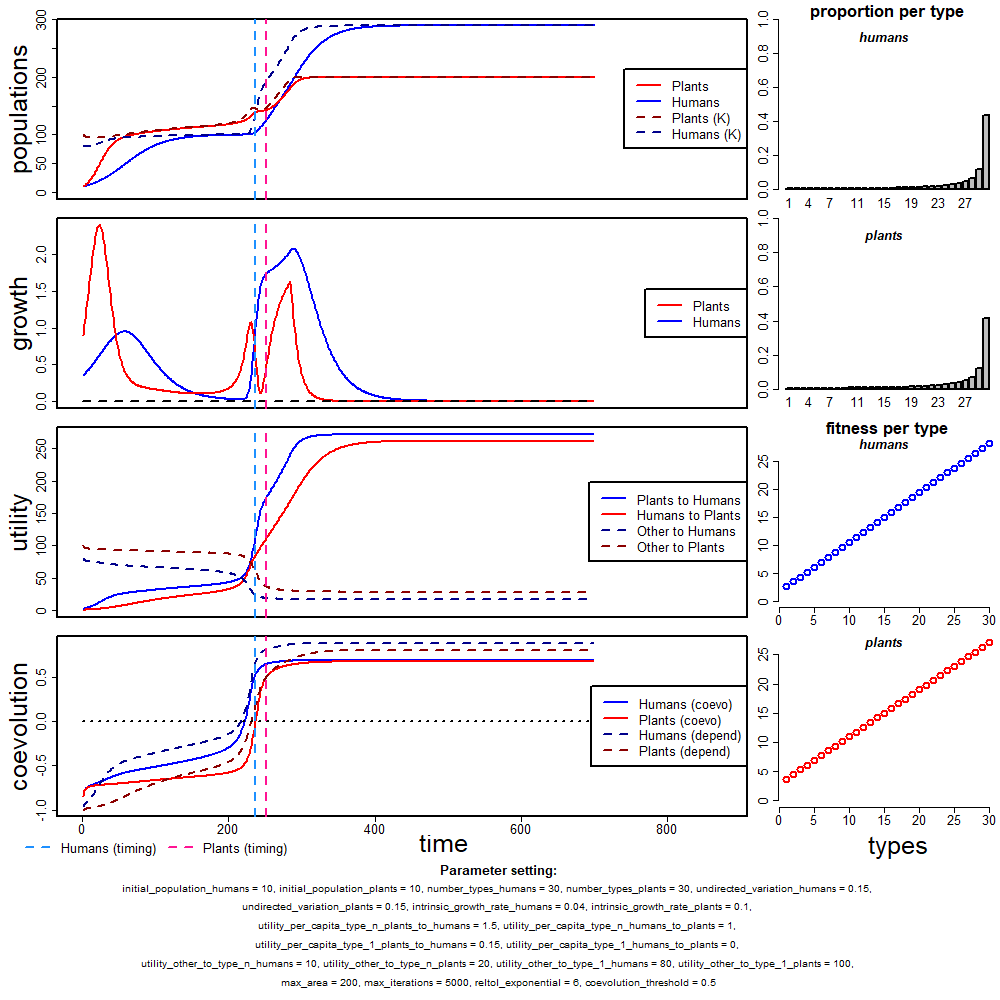
\includegraphics[width=1\linewidth]{plots/1_singleRun_coevolution-sameTiming_defaultPlot} \caption{Plotting the end state, i.e. both populations become stationary}\label{fig:1runcoevolutionsametimingdefaultplot}
\end{figure}

\newpage

\begin{figure}
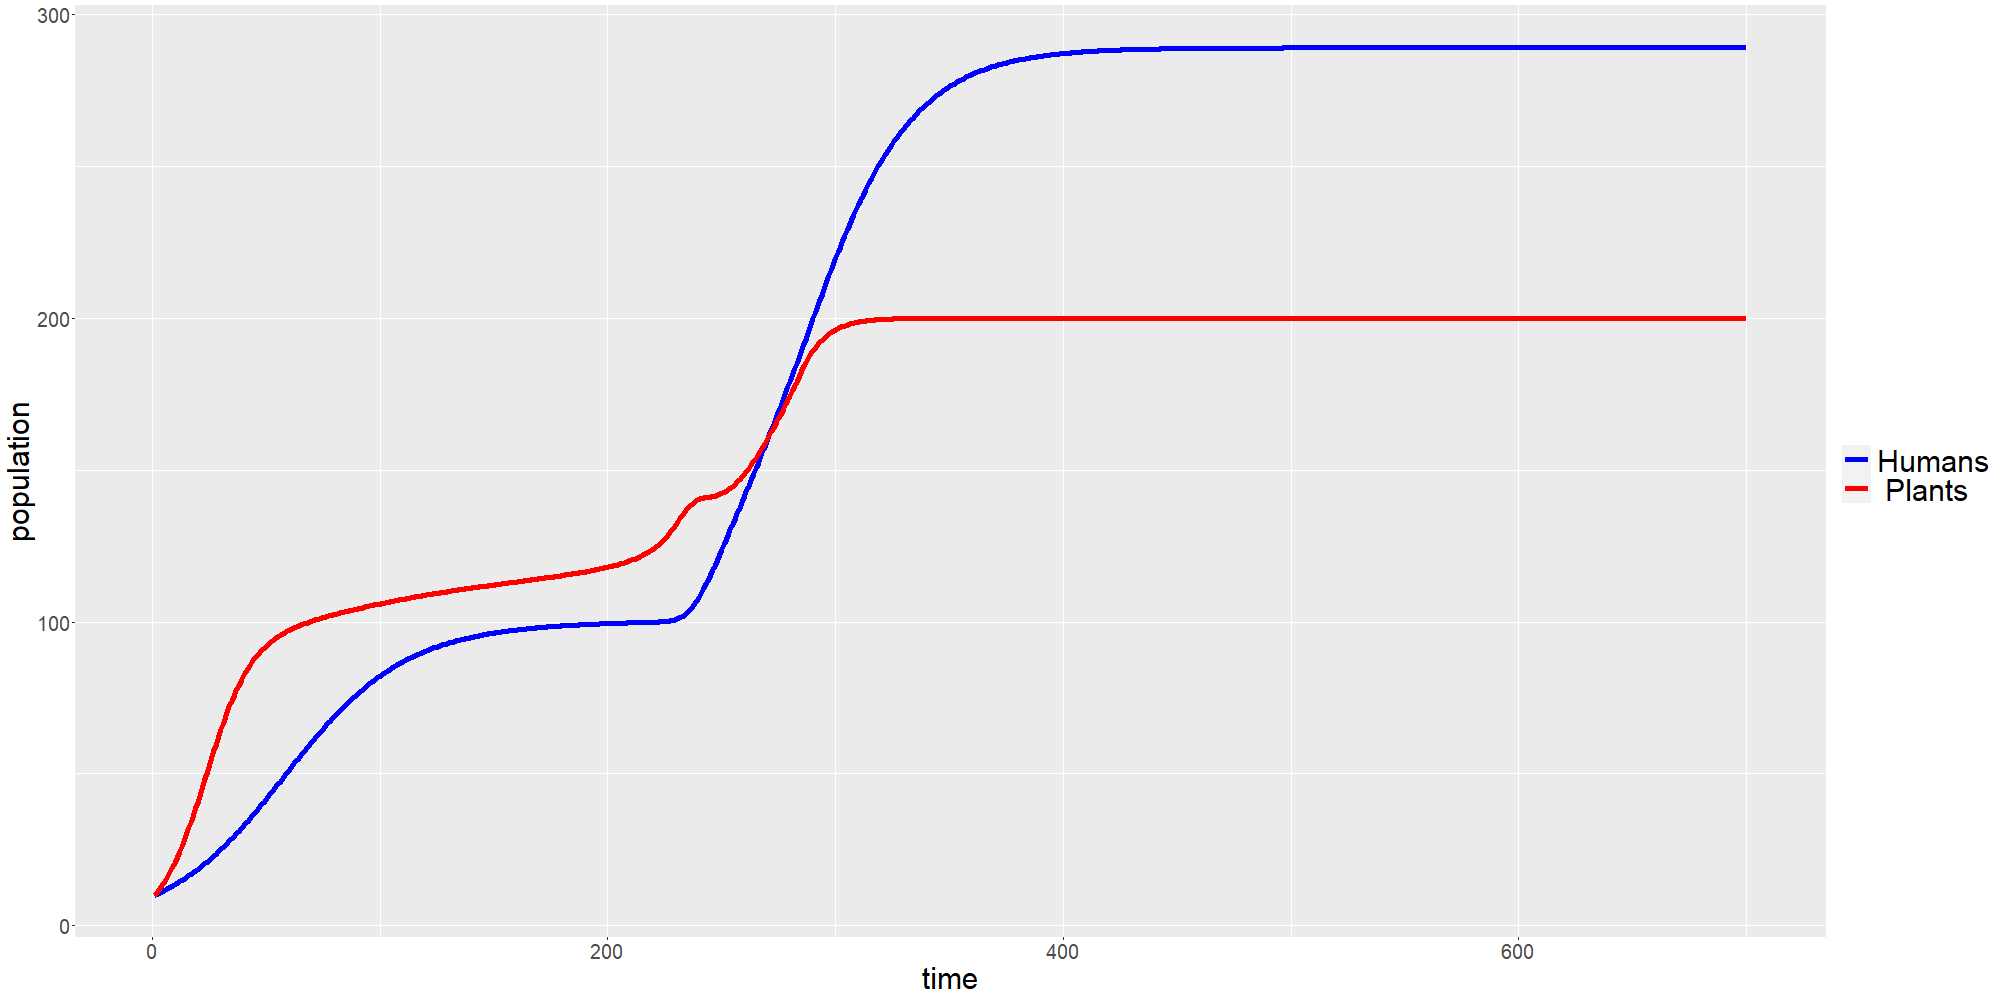
\includegraphics[width=1\linewidth]{plots/1_singleRun_coevolution-sameTiming_ggplot} \caption{Plotting population trajectories with ggplot2}\label{fig:1runcoevolutionsametimingggplotprint}
\end{figure}

\newpage

\FloatBarrier
\newpage

\hypertarget{no-coevolution}{%
\section{No coevolution}\label{no-coevolution}}

\includegraphics{hpcModel-exploration_files/figure-latex/1_run_noCoevolution-plot-1.pdf}

\newpage

\hypertarget{coevolution-with-early-cultivation}{%
\section{Coevolution with early cultivation}\label{coevolution-with-early-cultivation}}

\includegraphics{hpcModel-exploration_files/figure-latex/1_run_coevolution_earlyHumanChange-plot-1.pdf}

\newpage

\hypertarget{coevolution-with-early-domestication}{%
\section{Coevolution with early domestication}\label{coevolution-with-early-domestication}}

\includegraphics{hpcModel-exploration_files/figure-latex/1_run_coevolution_earlyPlantChange-plot-1.pdf}

\newpage

\hypertarget{cultivation-without-domestication}{%
\section{Cultivation without domestication}\label{cultivation-without-domestication}}

\includegraphics{hpcModel-exploration_files/figure-latex/1_run_partialCoevolution_noPlantChange-plot-1.pdf}

\newpage

\hypertarget{coevolution-with-population-bleep}{%
\section{Coevolution with population ``bleep''}\label{coevolution-with-population-bleep}}

\includegraphics{hpcModel-exploration_files/figure-latex/1_run_coevolution_bleep-plot-1.pdf}

\newpage

\hypertarget{coevolution-with-population-boom}{%
\section{Coevolution with population ``boom''}\label{coevolution-with-population-boom}}

\includegraphics{hpcModel-exploration_files/figure-latex/1_run_coevolution_boom-plot-1.pdf}

\newpage

\hypertarget{coevolution-with-long-population-boom}{%
\section{Coevolution with long population ``boom''}\label{coevolution-with-long-population-boom}}

\includegraphics{hpcModel-exploration_files/figure-latex/1_run_coevolution_longBoom-plot-1.pdf}

\newpage

\hypertarget{semi-coevolution-stationary-point}{%
\section{Semi-coevolution (stationary point)}\label{semi-coevolution-stationary-point}}

\includegraphics{hpcModel-exploration_files/figure-latex/1_run_partialCoevolution-plot-1.pdf}

\newpage

\hypertarget{semi-coevolution-oscillations}{%
\section{Semi-coevolution (oscillations)}\label{semi-coevolution-oscillations}}

\includegraphics{hpcModel-exploration_files/figure-latex/1_run_partialCoevolution_oscillation1-plot-1.pdf}

\includegraphics{hpcModel-exploration_files/figure-latex/1_run_partialCoevolution_oscillation2-plot-1.pdf}

\hypertarget{one-parameter-exploration}{%
\chapter{One parameter exploration}\label{one-parameter-exploration}}

\newpage

\hypertarget{full-example-tableplot-alternatives}{%
\section{Full example (table+plot alternatives)}\label{full-example-tableplot-alternatives}}

\hypertarget{utility-per-capita-of-type-n-plants-to-humans-baru_p_nh}{%
\subsection{\texorpdfstring{utility per capita \textbf{of} type n plants \textbf{to} humans (\(\bar{U}_{P_{n}H}\)):}{utility per capita of type n plants to humans (\textbackslash bar\{U\}\_\{P\_\{n\}H\}):}}\label{utility-per-capita-of-type-n-plants-to-humans-baru_p_nh}}

\begin{verbatim}
## [1] 31
## [1] 31
\end{verbatim}

\begin{table}[!h]

\caption{\label{tab:2mUPnHtablepdf}Parameter setting}
\centering
\begin{tabular}[t]{l|l}
\hline
parameter & value\\
\hline
initial\_population\_humans & 10\\
\hline
initial\_population\_plants & 10\\
\hline
number\_types\_humans & 30\\
\hline
number\_types\_plants & 30\\
\hline
undirected\_variation\_humans & 0.15\\
\hline
undirected\_variation\_plants & 0.15\\
\hline
intrinsic\_growth\_rate\_humans & 0.04\\
\hline
intrinsic\_growth\_rate\_plants & 0.1\\
\hline
utility\_per\_capita\_type\_n\_plants\_to\_humans & 0.5 - 2.5 (sample = 100 )\\
\hline
utility\_per\_capita\_type\_n\_humans\_to\_plants & 1\\
\hline
utility\_per\_capita\_type\_1\_plants\_to\_humans & 0.15\\
\hline
utility\_per\_capita\_type\_1\_humans\_to\_plants & 0\\
\hline
utility\_other\_to\_type\_n\_humans & 10\\
\hline
utility\_other\_to\_type\_n\_plants & 20\\
\hline
utility\_other\_to\_type\_1\_humans & 80\\
\hline
utility\_other\_to\_type\_1\_plants & 100\\
\hline
max\_area & 200\\
\hline
max\_iterations & 5000\\
\hline
reltol\_exponential & 6\\
\hline
coevolution\_threshold & 0.5\\
\hline
humans & 89.8095348728372 - 472.074840353865 (sample = 100 )\\
\hline
plants & 104.041173556269 - 200 (sample = 45 )\\
\hline
coevolution\_coefficient\_humans & -0.618988585806422 - 0.698779265650612 (sample = 100 )\\
\hline
coevolution\_coefficient\_plants & -0.67653715347976 - 0.690301736910053 (sample = 100 )\\
\hline
dependency\_coefficient\_humans & -0.569716349279568 - 0.931253547354916 (sample = 100 )\\
\hline
dependency\_coefficient\_plants & -0.765398002302459 - 0.879740522206507 (sample = 100 )\\
\hline
timing\_humans & 0 - 574 (sample = 56 )\\
\hline
timing\_plants & 0 - 591 (sample = 54 )\\
\hline
time\_end & 431 - 1189 (sample = 86 )\\
\hline
adaptativeCost.H & 0\\
\hline
adaptativeCost.P & 0\\
\hline
\end{tabular}
\end{table}

\begin{figure}
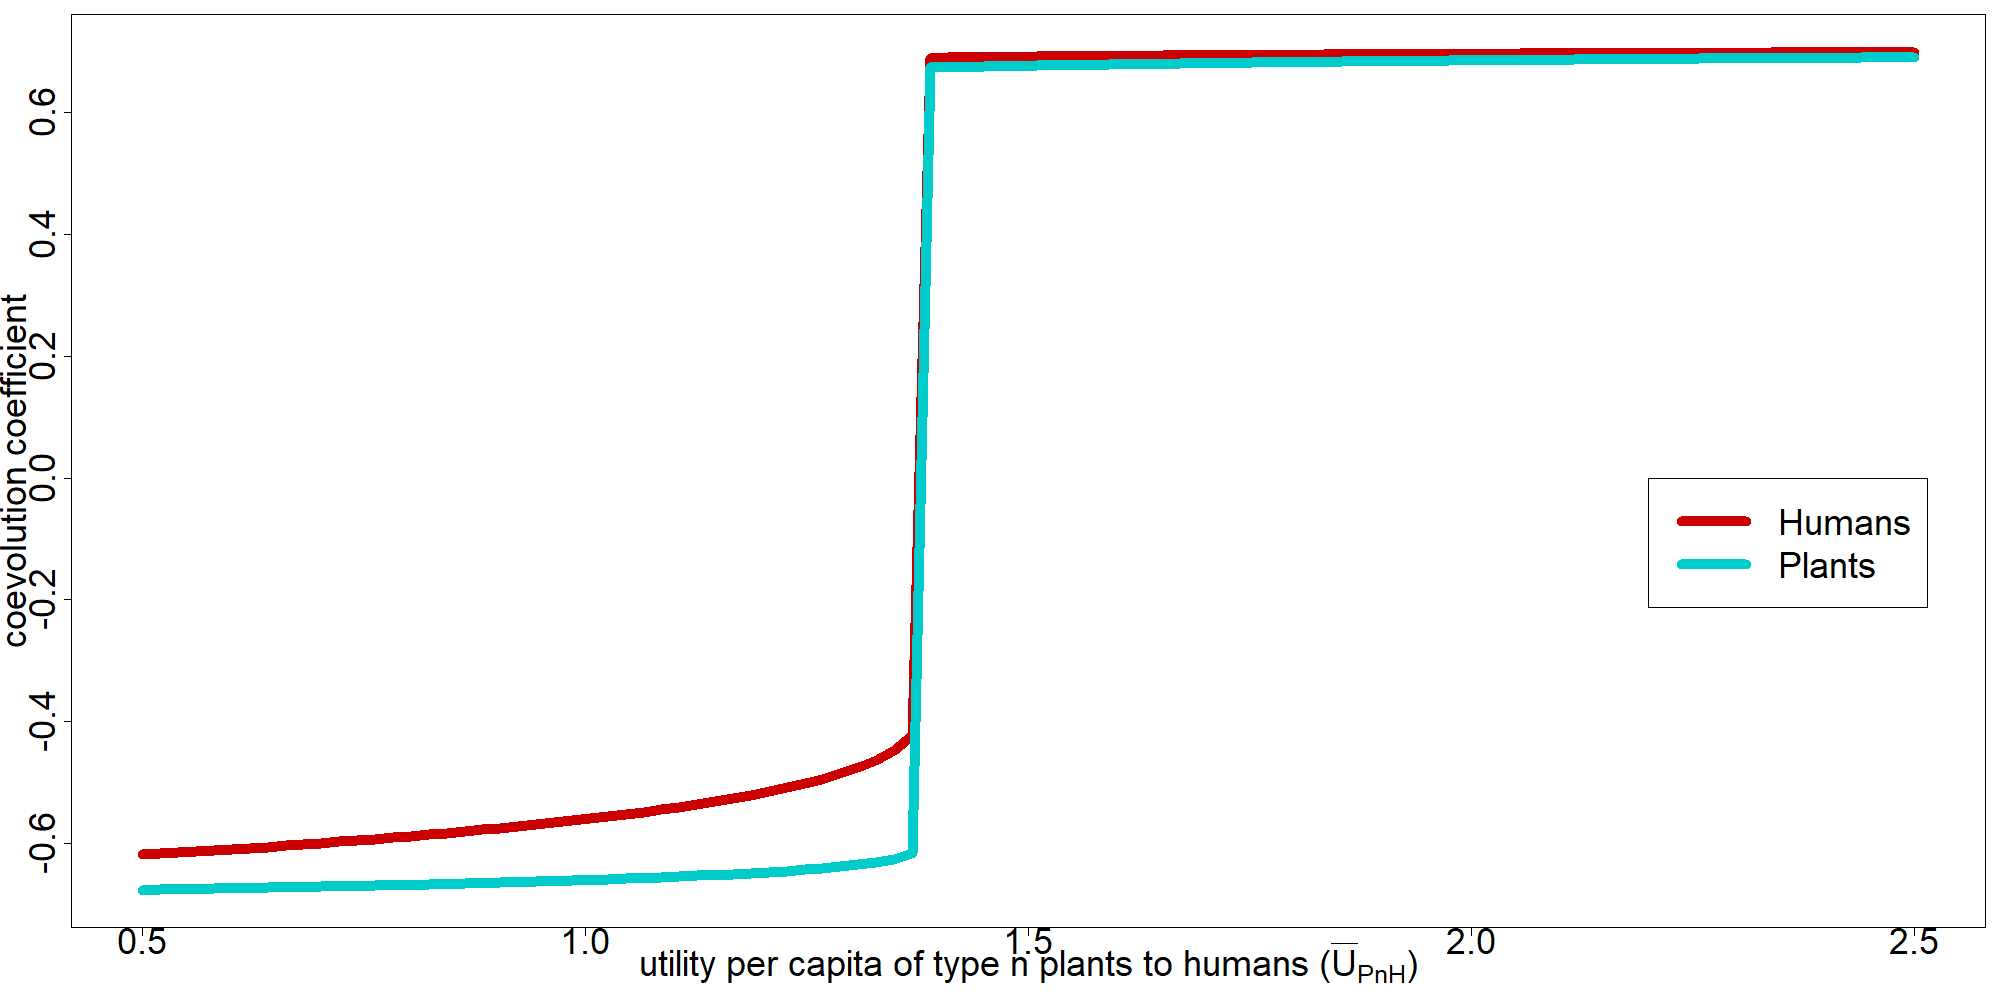
\includegraphics[width=1\linewidth]{plots/2_exp_utility_per_capita_type_n_plants_to_humans_bifurcationPlotSimple} \caption{Bifurcation plot (ggplot2)}\label{fig:2mUPnHbifplot1print}
\end{figure}

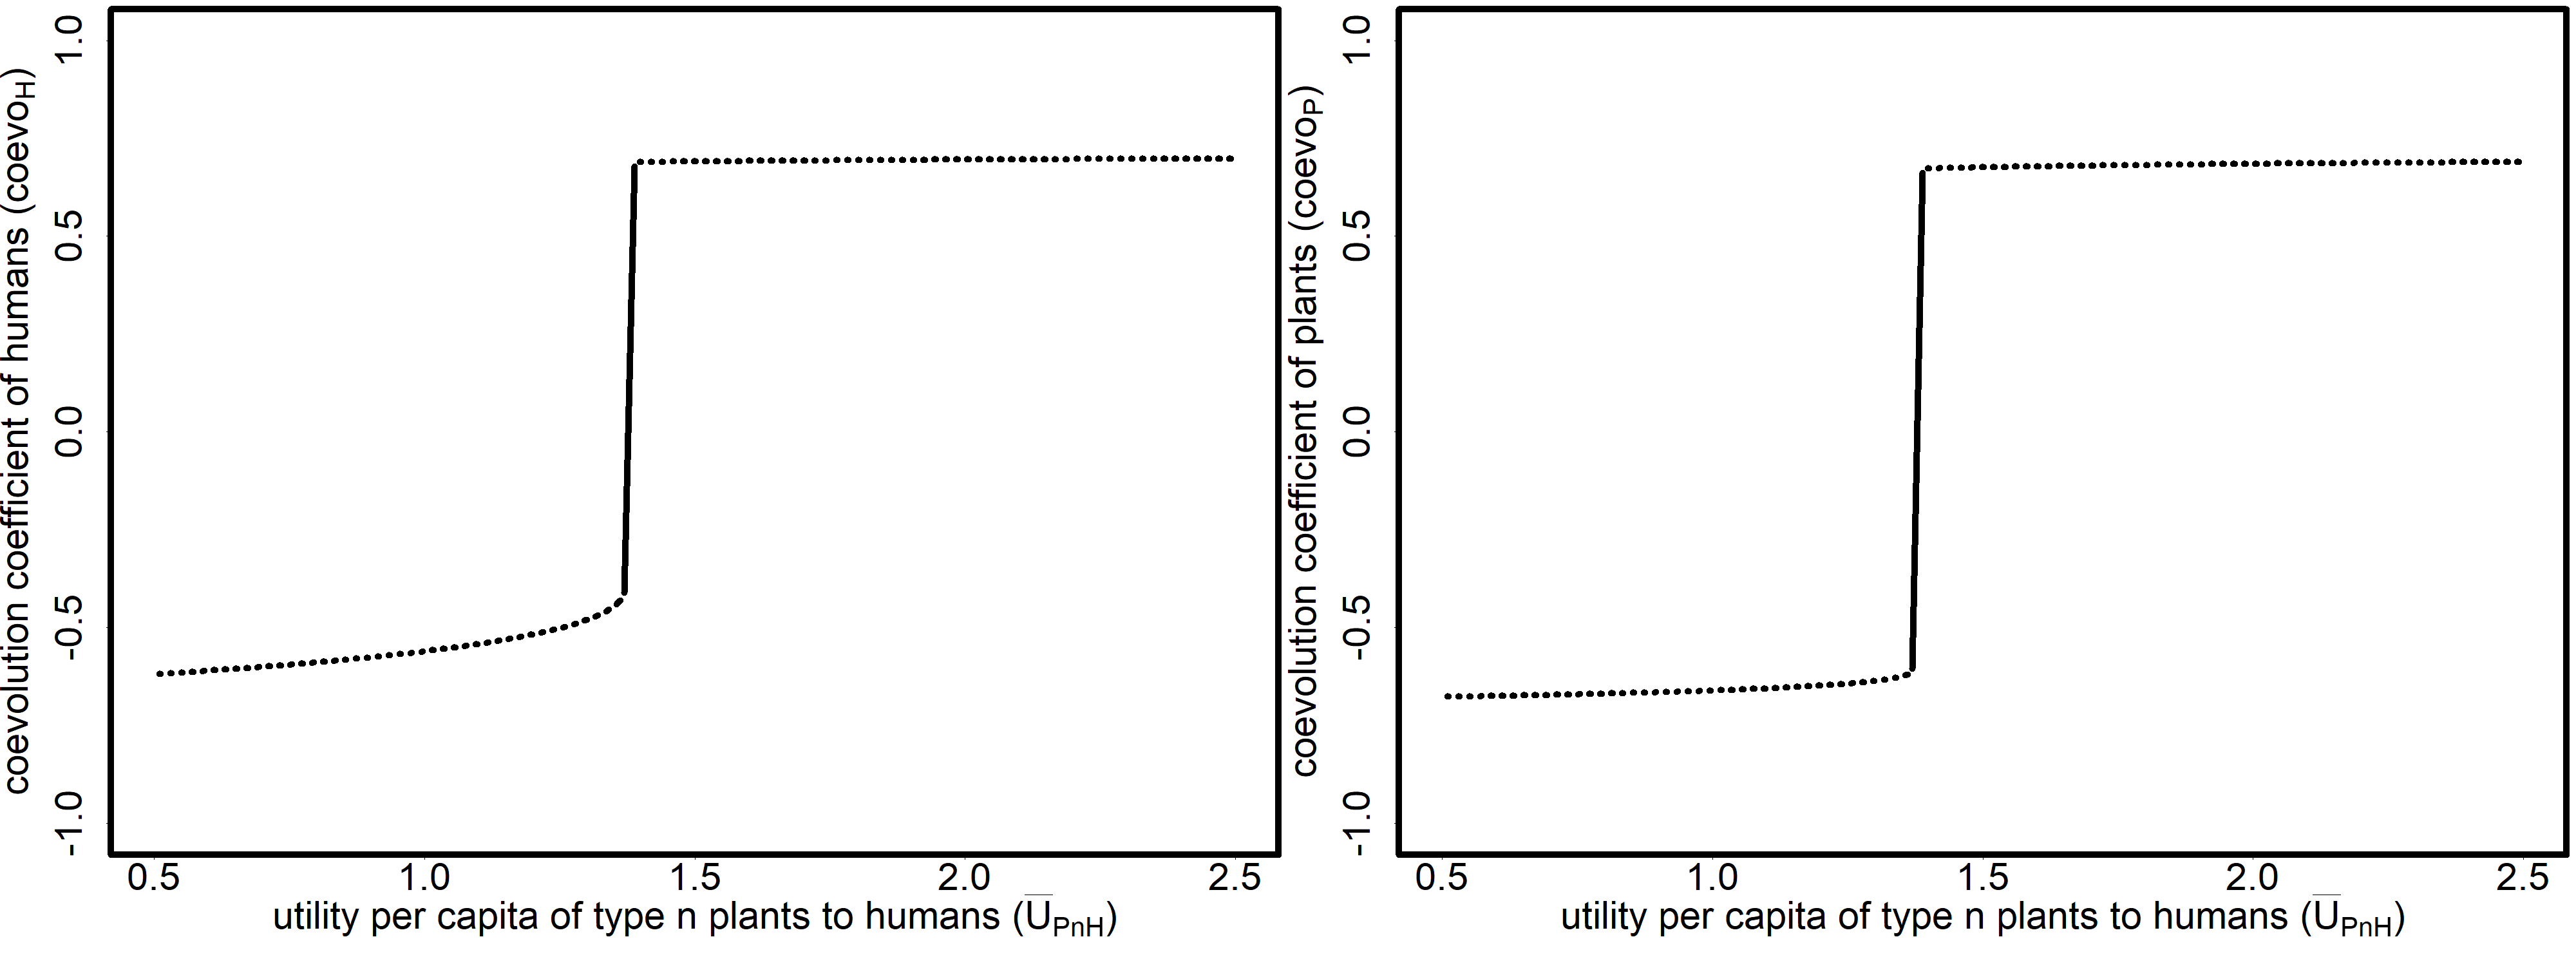
\includegraphics[width=1\linewidth]{plots/2_exp_utility_per_capita_type_n_plants_to_humans_bifurcationPlotPair}

\newpage

\hypertarget{exploration-on-default-setting-for-each-parameter}{%
\section{Exploration on `default' setting for each parameter:}\label{exploration-on-default-setting-for-each-parameter}}

\hypertarget{initial-populations-of-humans-and-plants-init_hinit_p}{%
\subsection{\texorpdfstring{Initial populations of humans and plants (\(init_{H},\,init_{P}\))}{Initial populations of humans and plants (init\_\{H\},\textbackslash,init\_\{P\})}}\label{initial-populations-of-humans-and-plants-init_hinit_p}}

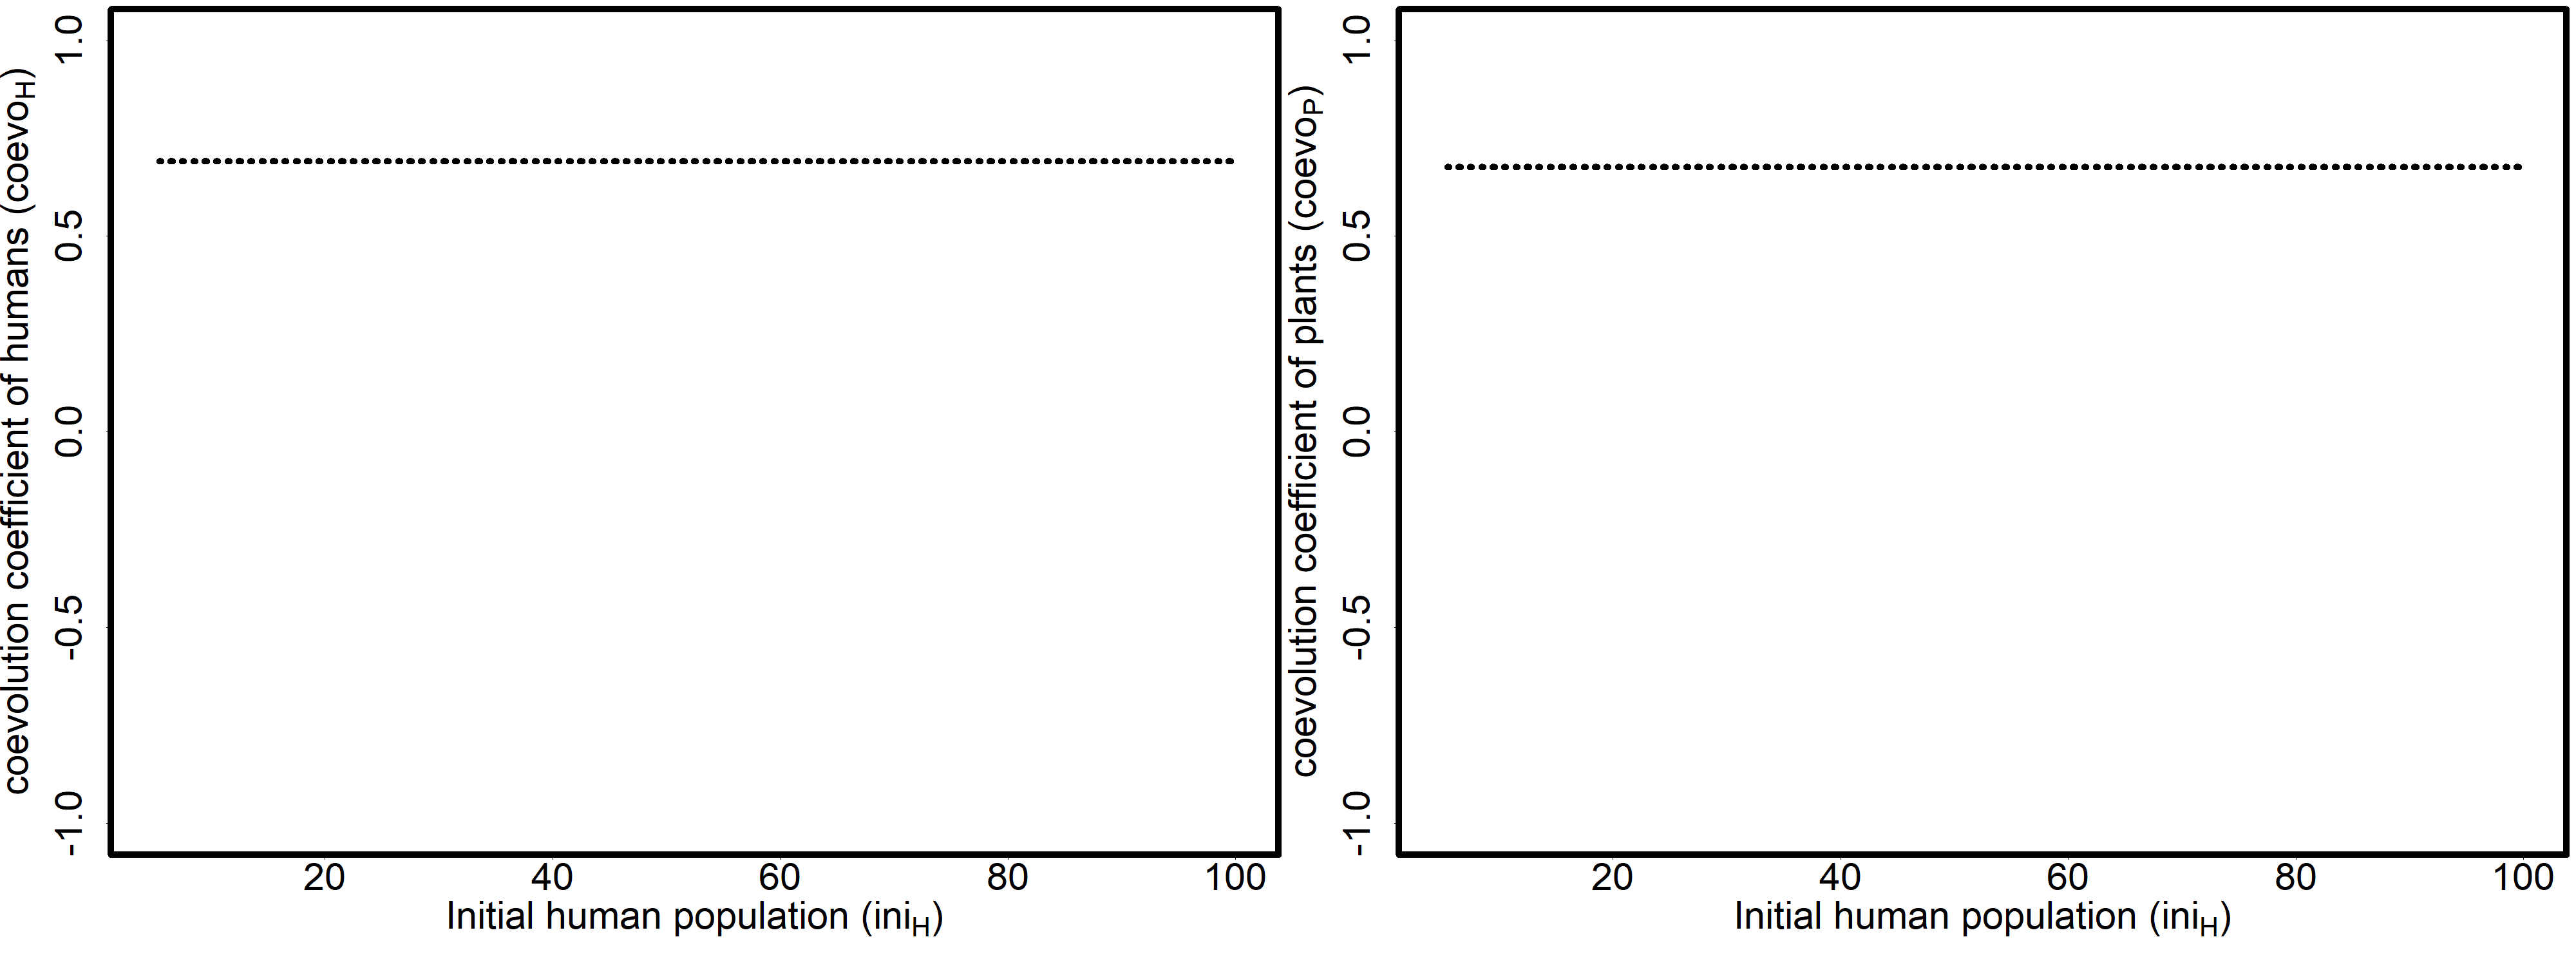
\includegraphics[width=1\linewidth]{plots/2_exp_initial_population_humans_bifurcationPlotPair}

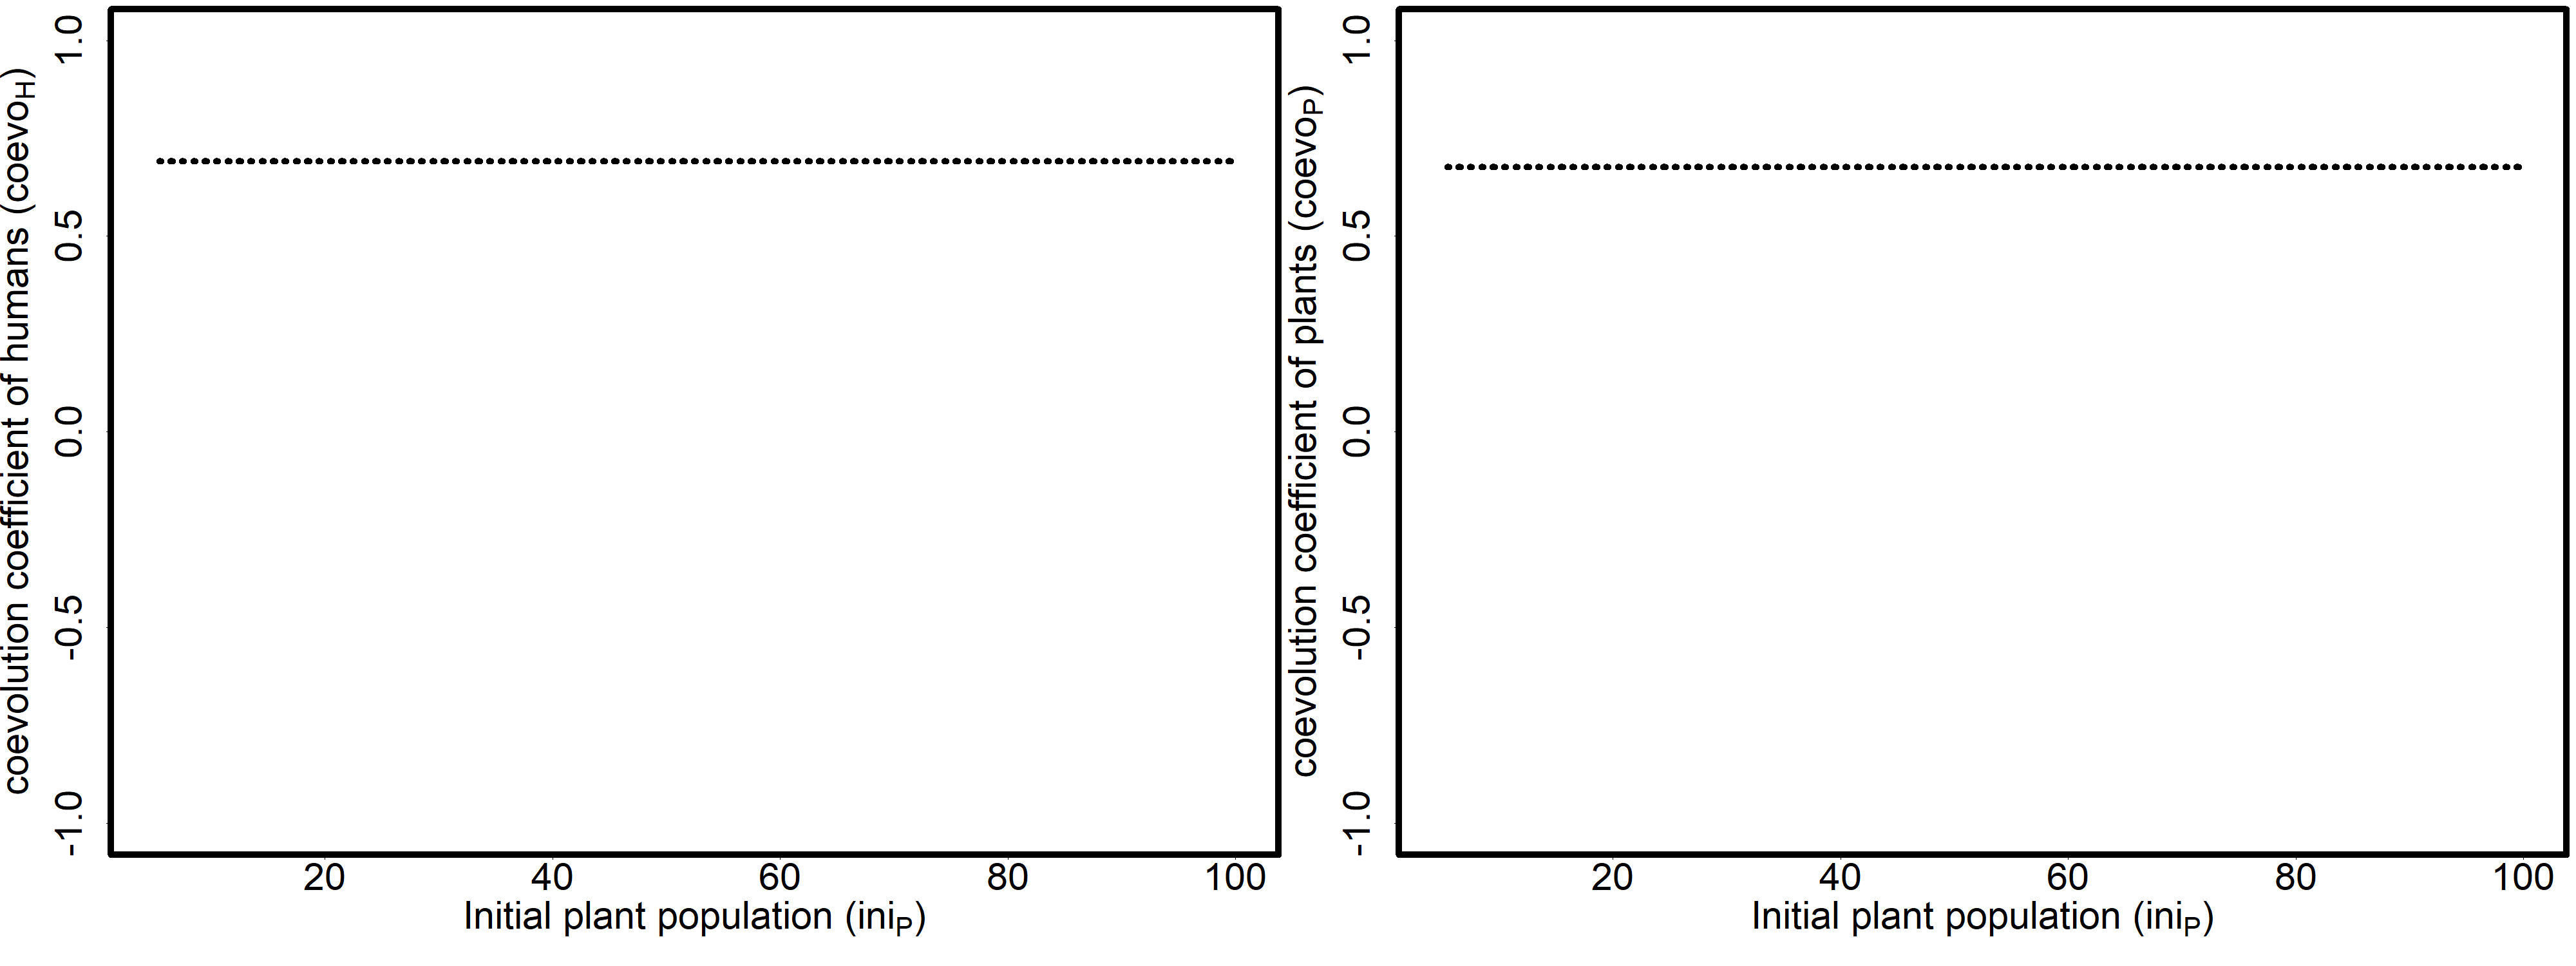
\includegraphics[width=1\linewidth]{plots/2_exp_initial_population_plants_bifurcationPlotPair}

\hypertarget{number-of-types-of-humans-and-plants-n_hn_p}{%
\subsection{\texorpdfstring{Number of types of humans and plants (\(n_{H},\,n_{P}\)):}{Number of types of humans and plants (n\_\{H\},\textbackslash,n\_\{P\}):}}\label{number-of-types-of-humans-and-plants-n_hn_p}}

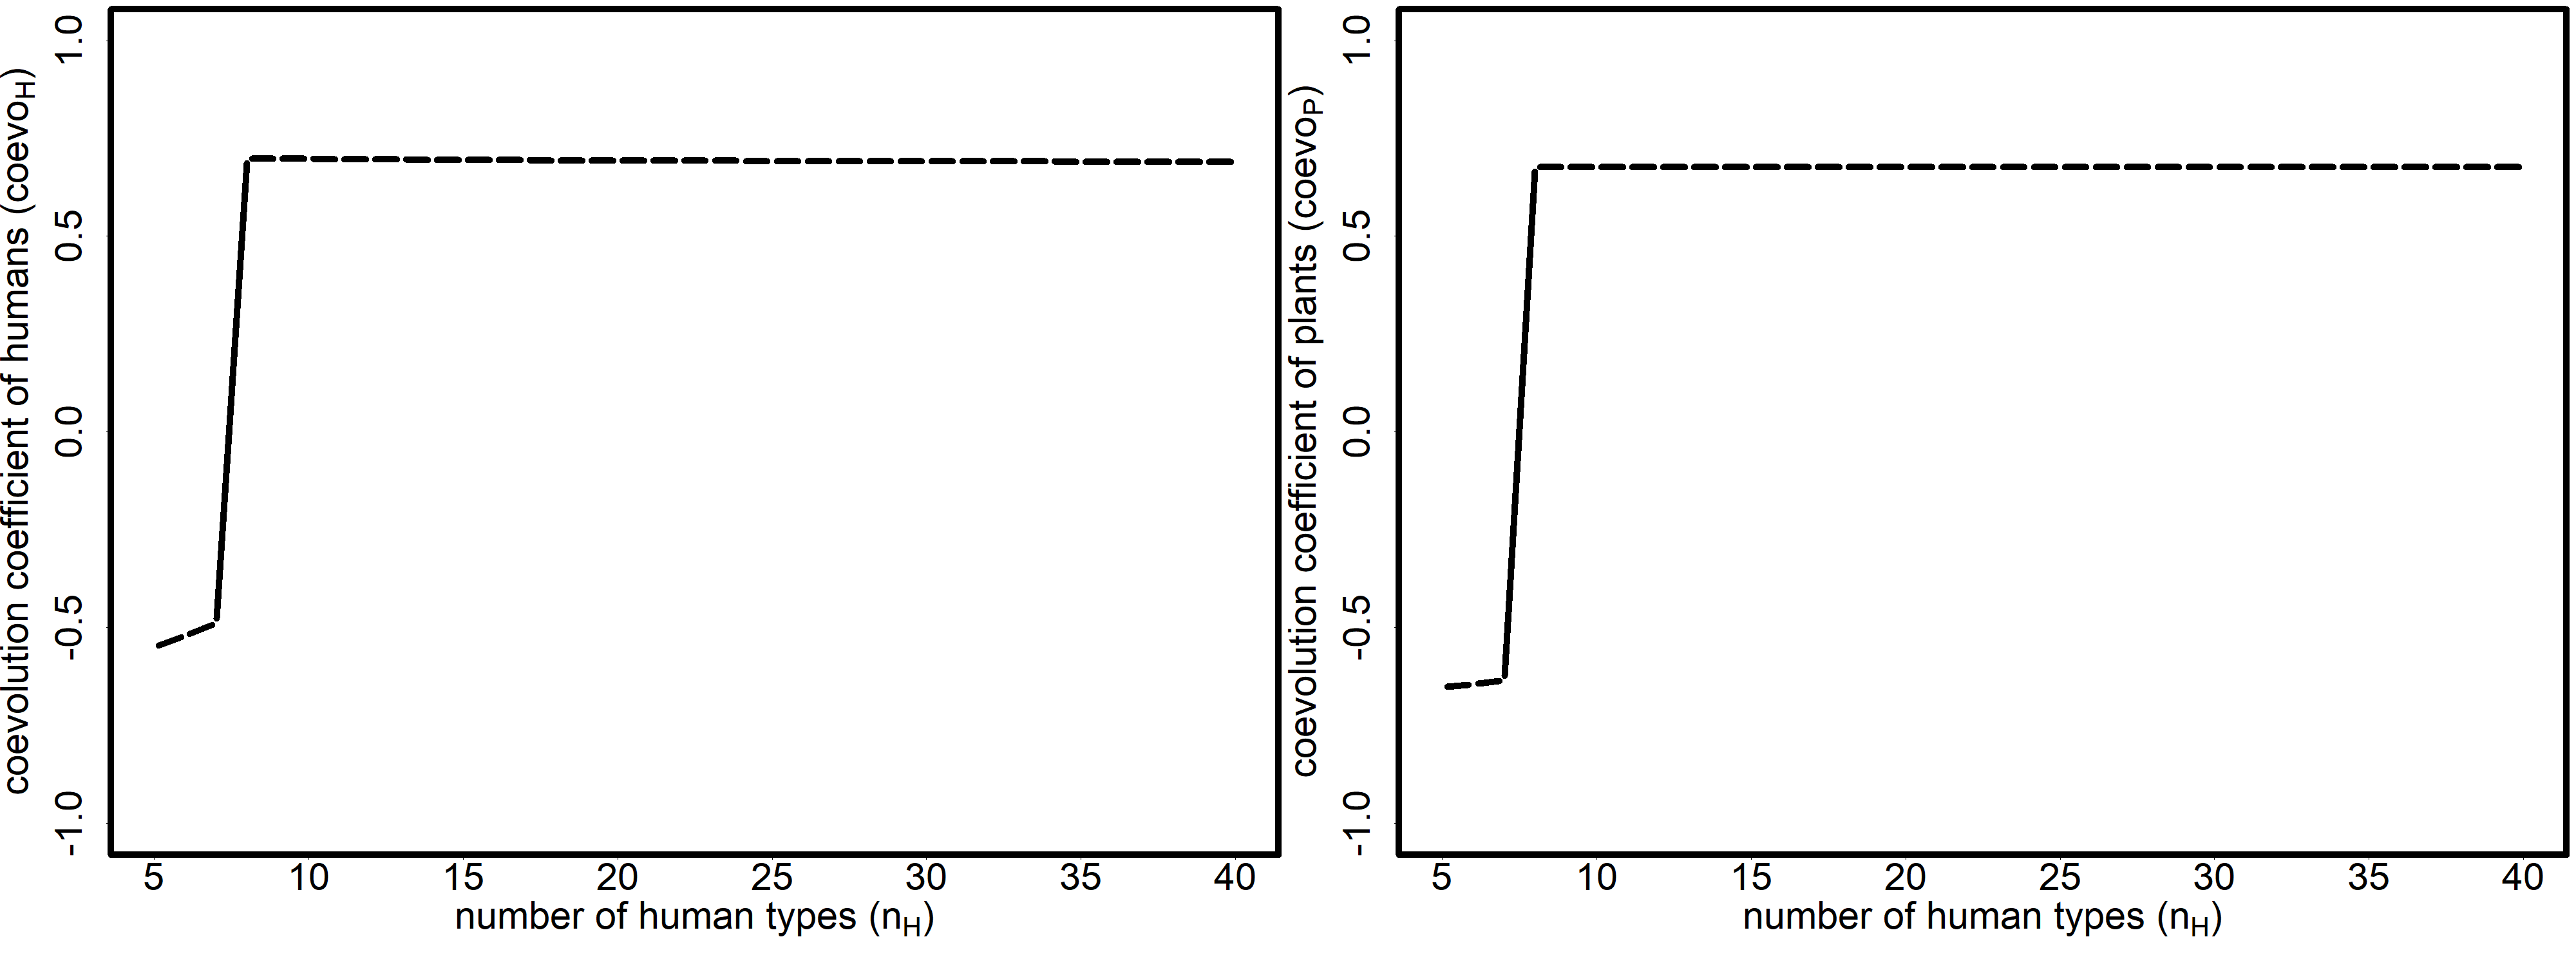
\includegraphics[width=1\linewidth]{plots/2_exp_number_types_humans_bifurcationPlotPair}

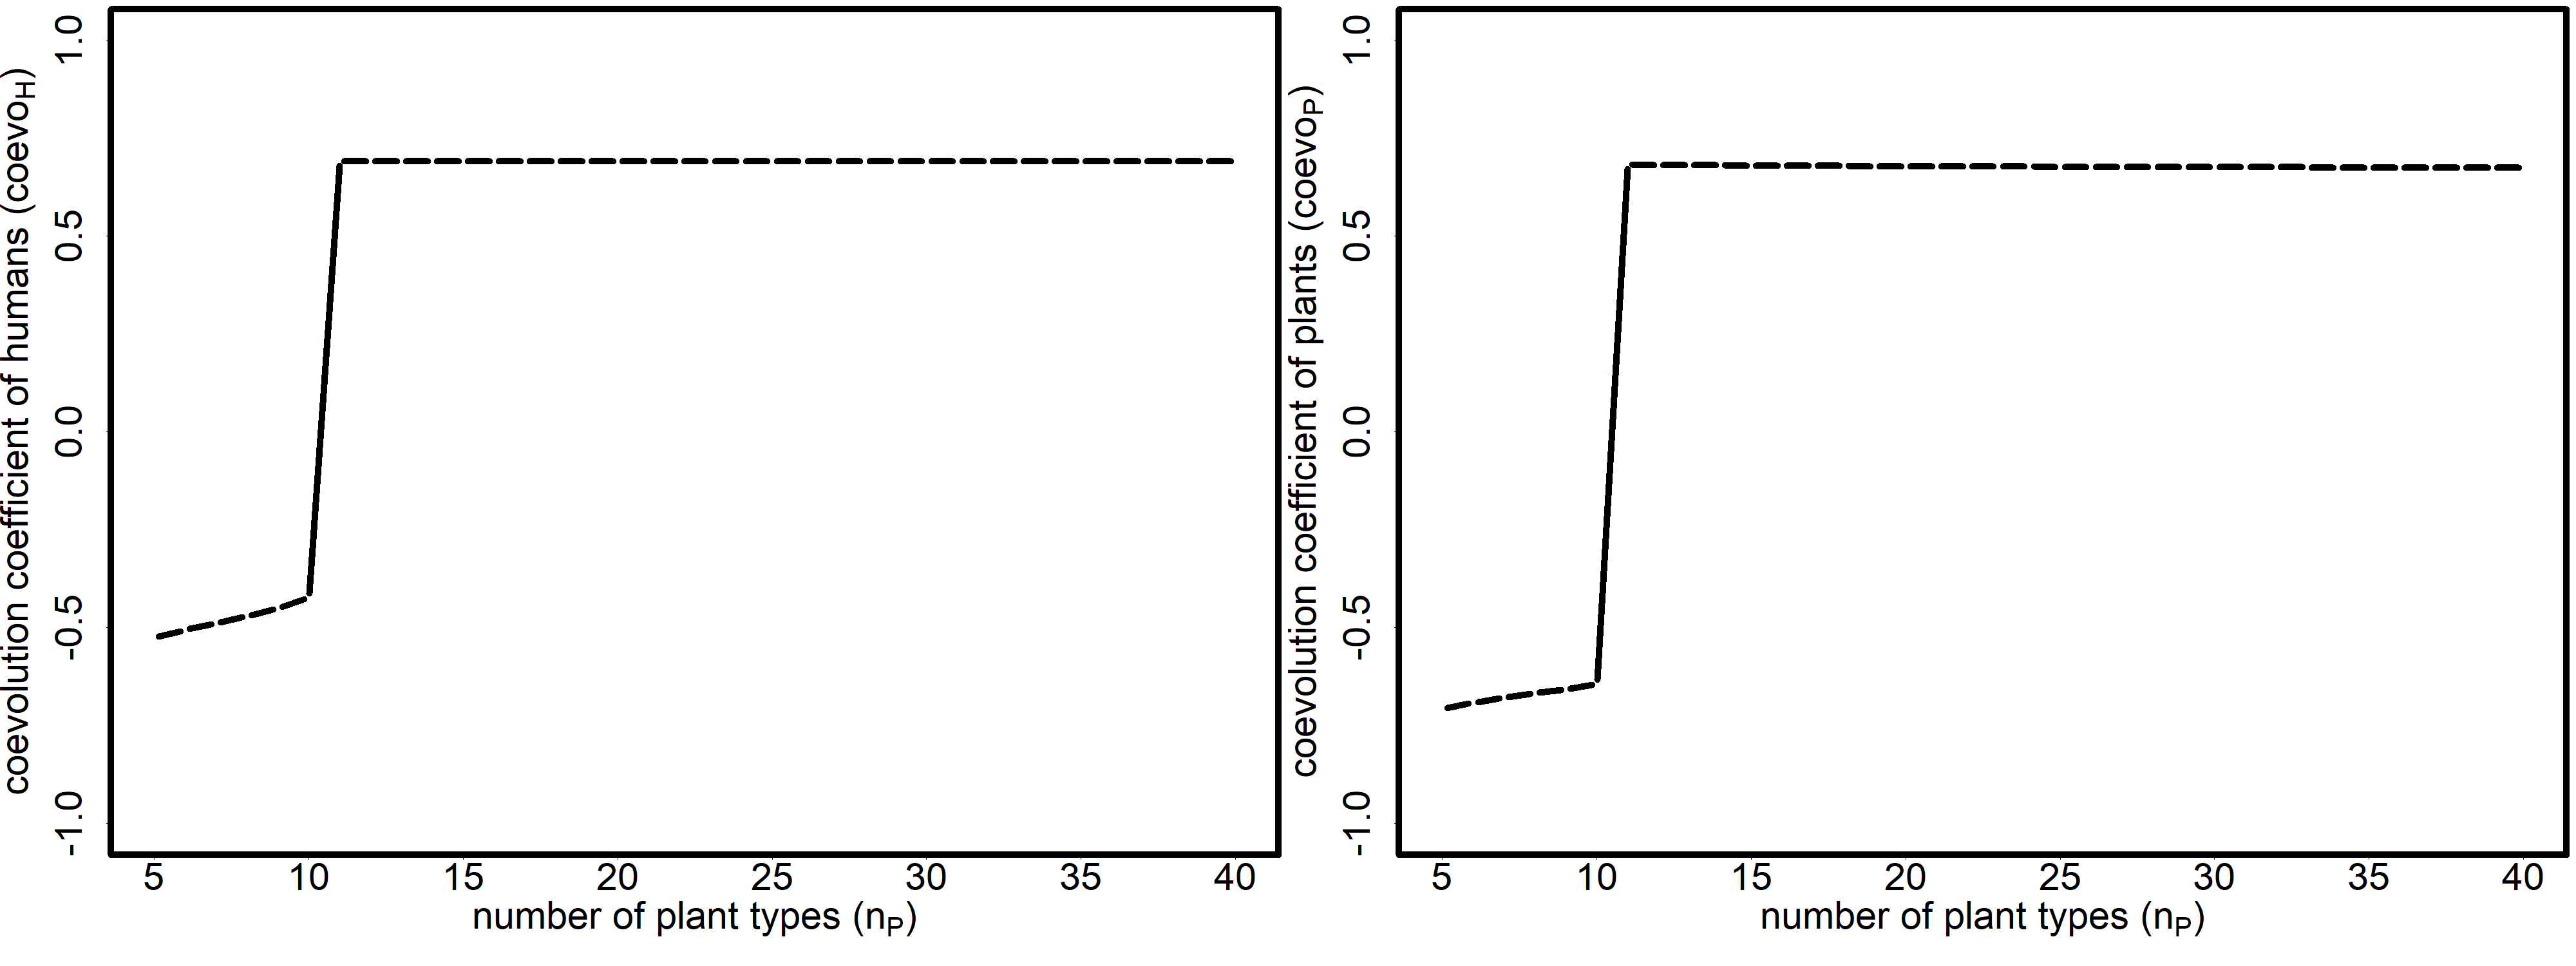
\includegraphics[width=1\linewidth]{plots/2_exp_number_types_plants_bifurcationPlotPair}

\hypertarget{level-of-undirected-variation-in-humans-and-plants-v_hv_p}{%
\subsection{\texorpdfstring{level of undirected variation in humans and plants (\(v_{H},\,v_{P}\)):}{level of undirected variation in humans and plants (v\_\{H\},\textbackslash,v\_\{P\}):}}\label{level-of-undirected-variation-in-humans-and-plants-v_hv_p}}

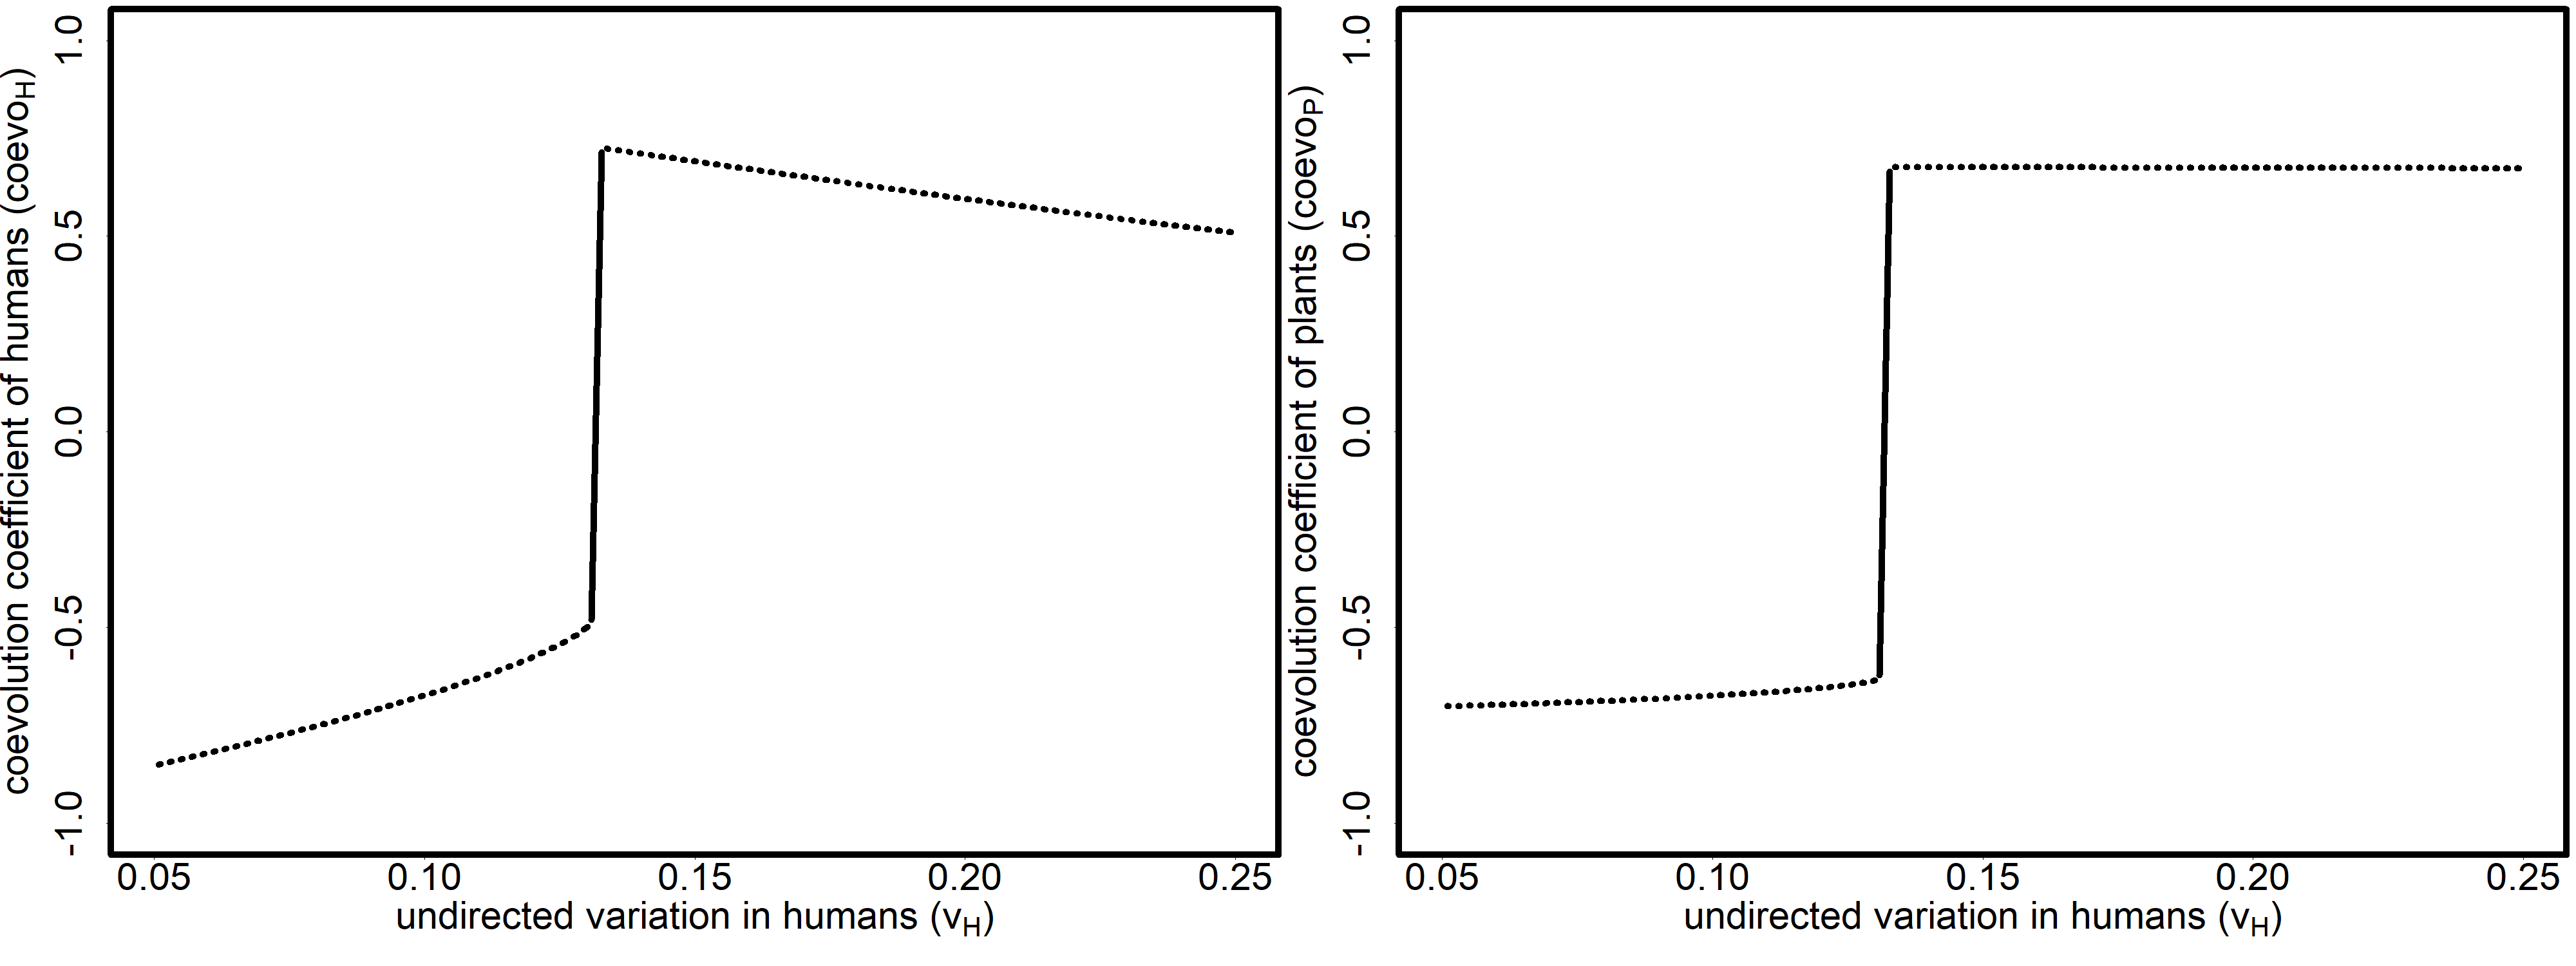
\includegraphics[width=1\linewidth]{plots/2_exp_undirected_variation_humans_bifurcationPlotPair}

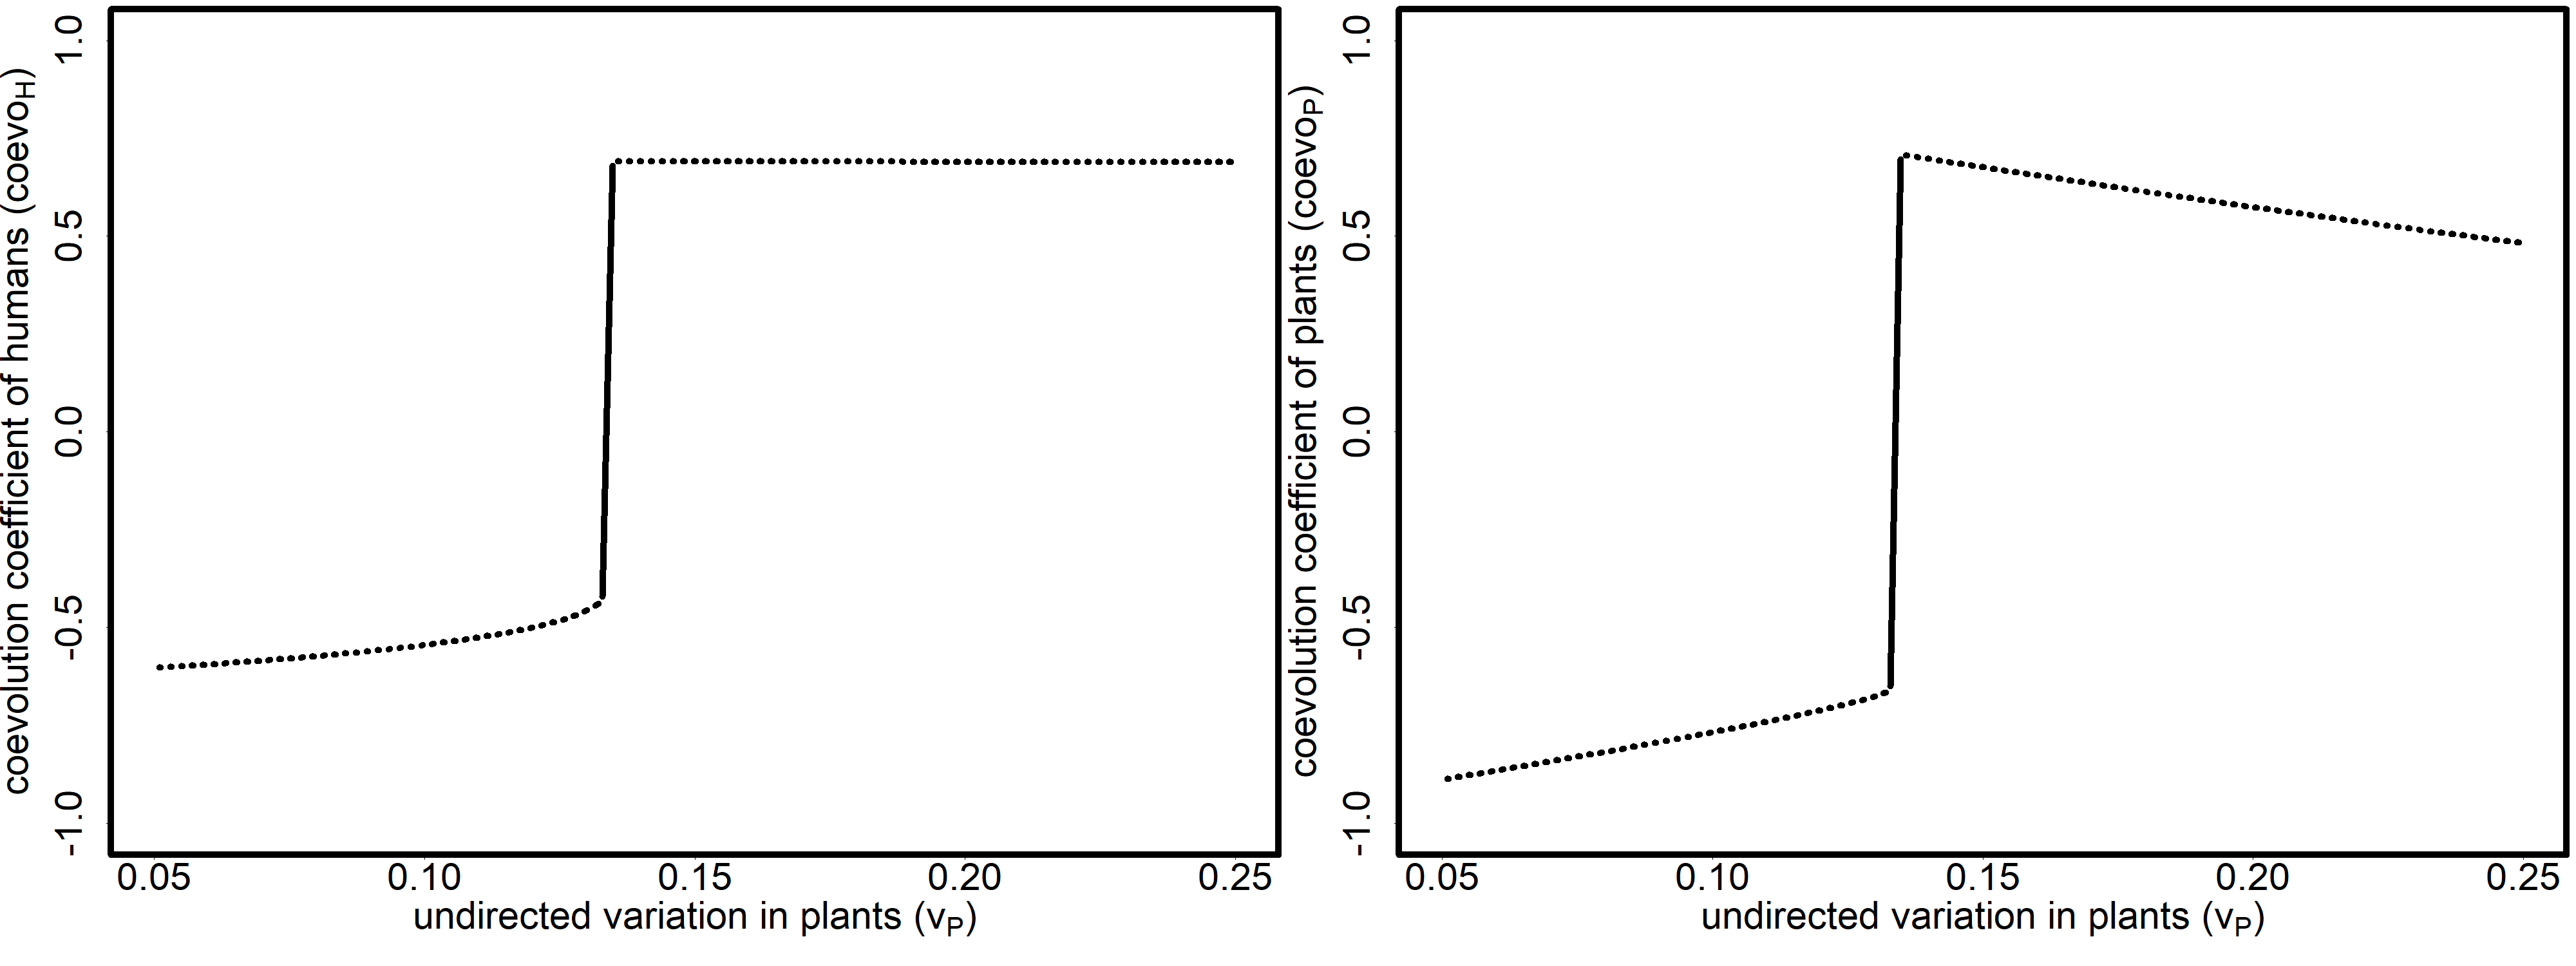
\includegraphics[width=1\linewidth]{plots/2_exp_undirected_variation_plants_bifurcationPlotPair}

\hypertarget{intrinsic-growth-rates-for-human-and-plant-populations-r_hr_p}{%
\subsection{\texorpdfstring{intrinsic growth rates for human and plant populations (\(r_{H},\,r_{P}\)):}{intrinsic growth rates for human and plant populations (r\_\{H\},\textbackslash,r\_\{P\}):}}\label{intrinsic-growth-rates-for-human-and-plant-populations-r_hr_p}}

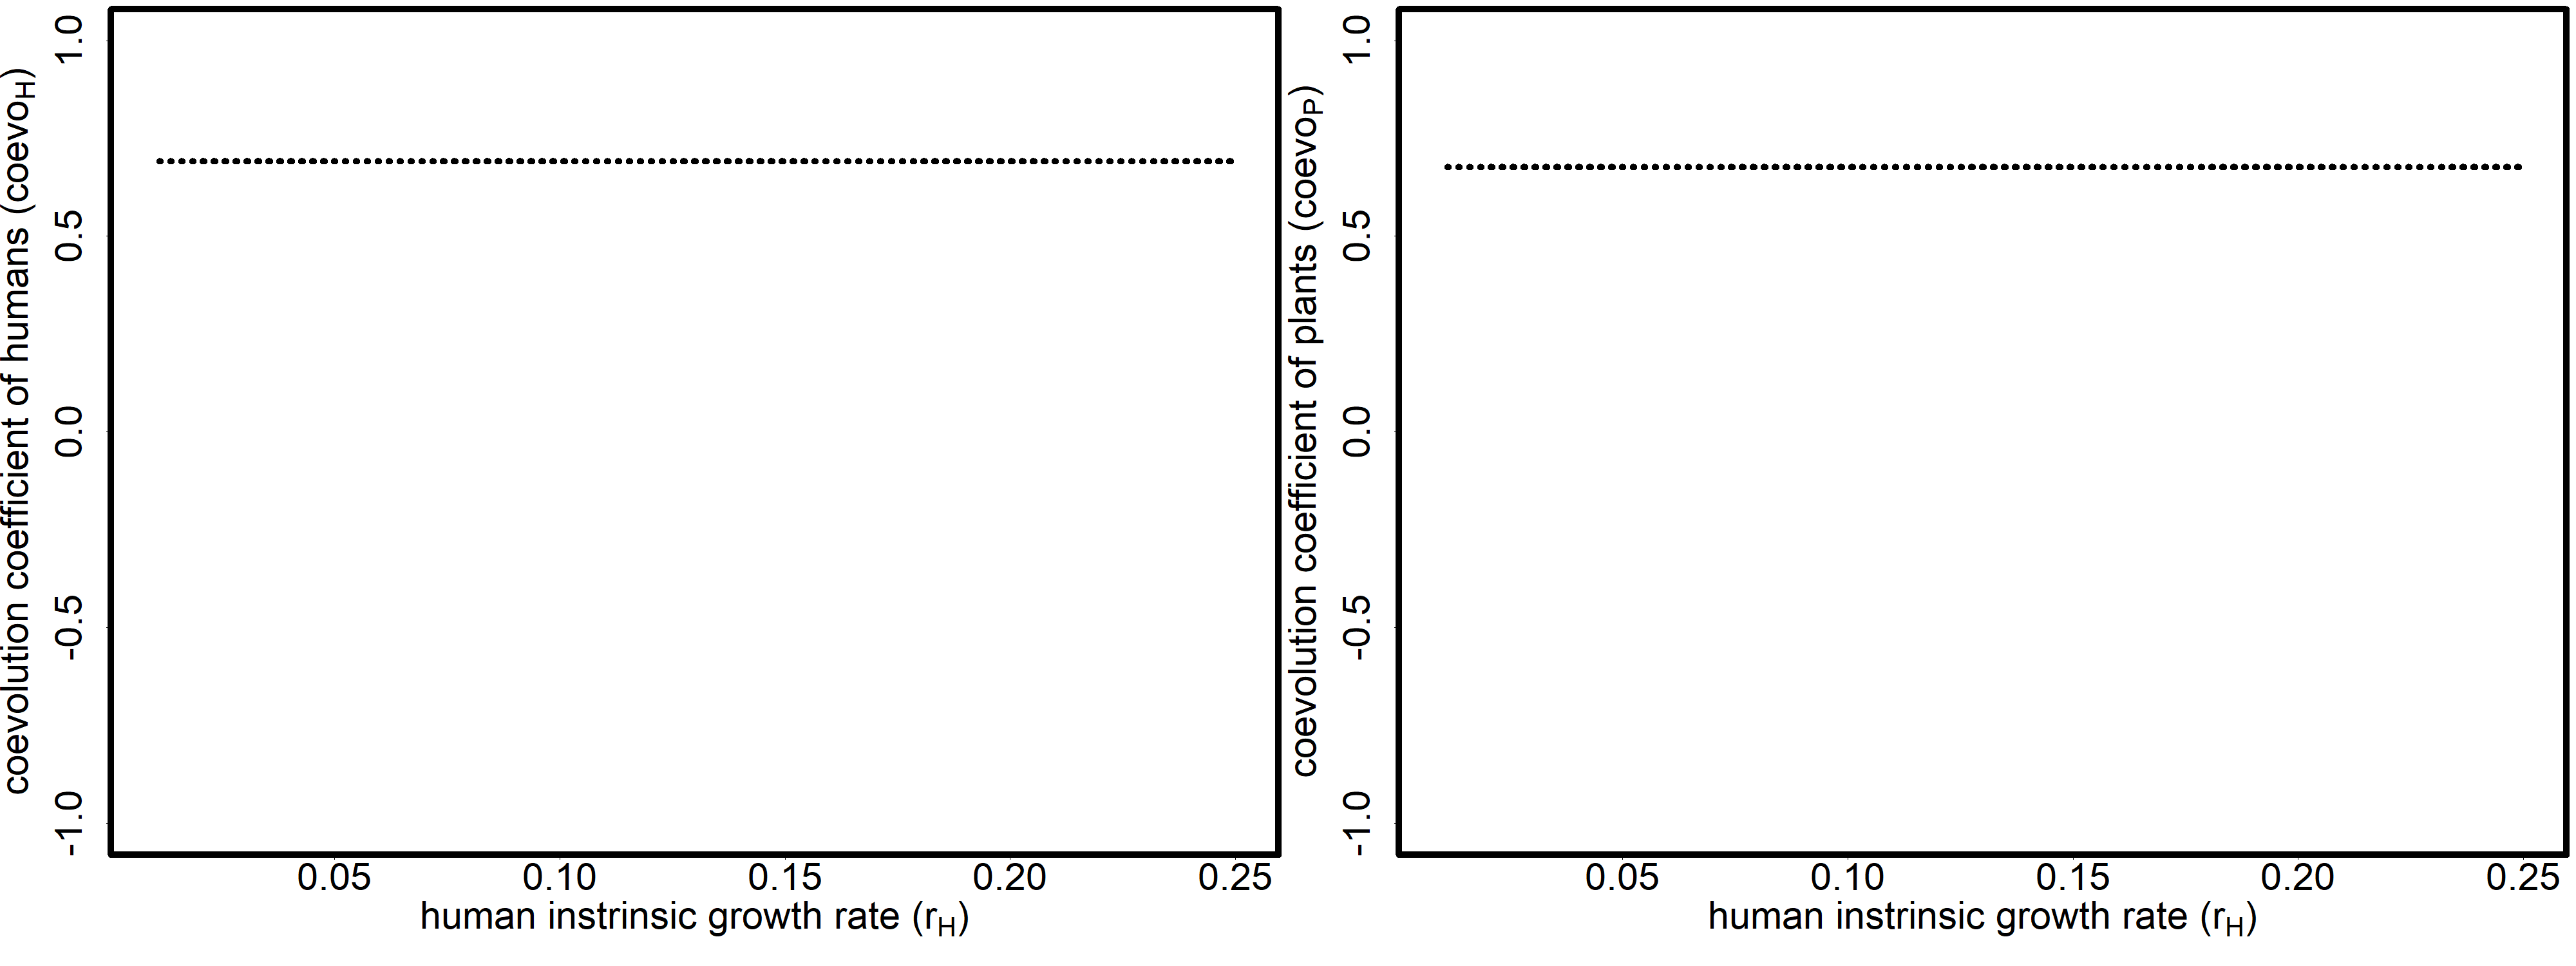
\includegraphics[width=1\linewidth]{plots/2_exp_intrinsic_growth_rate_humans_bifurcationPlotPair}

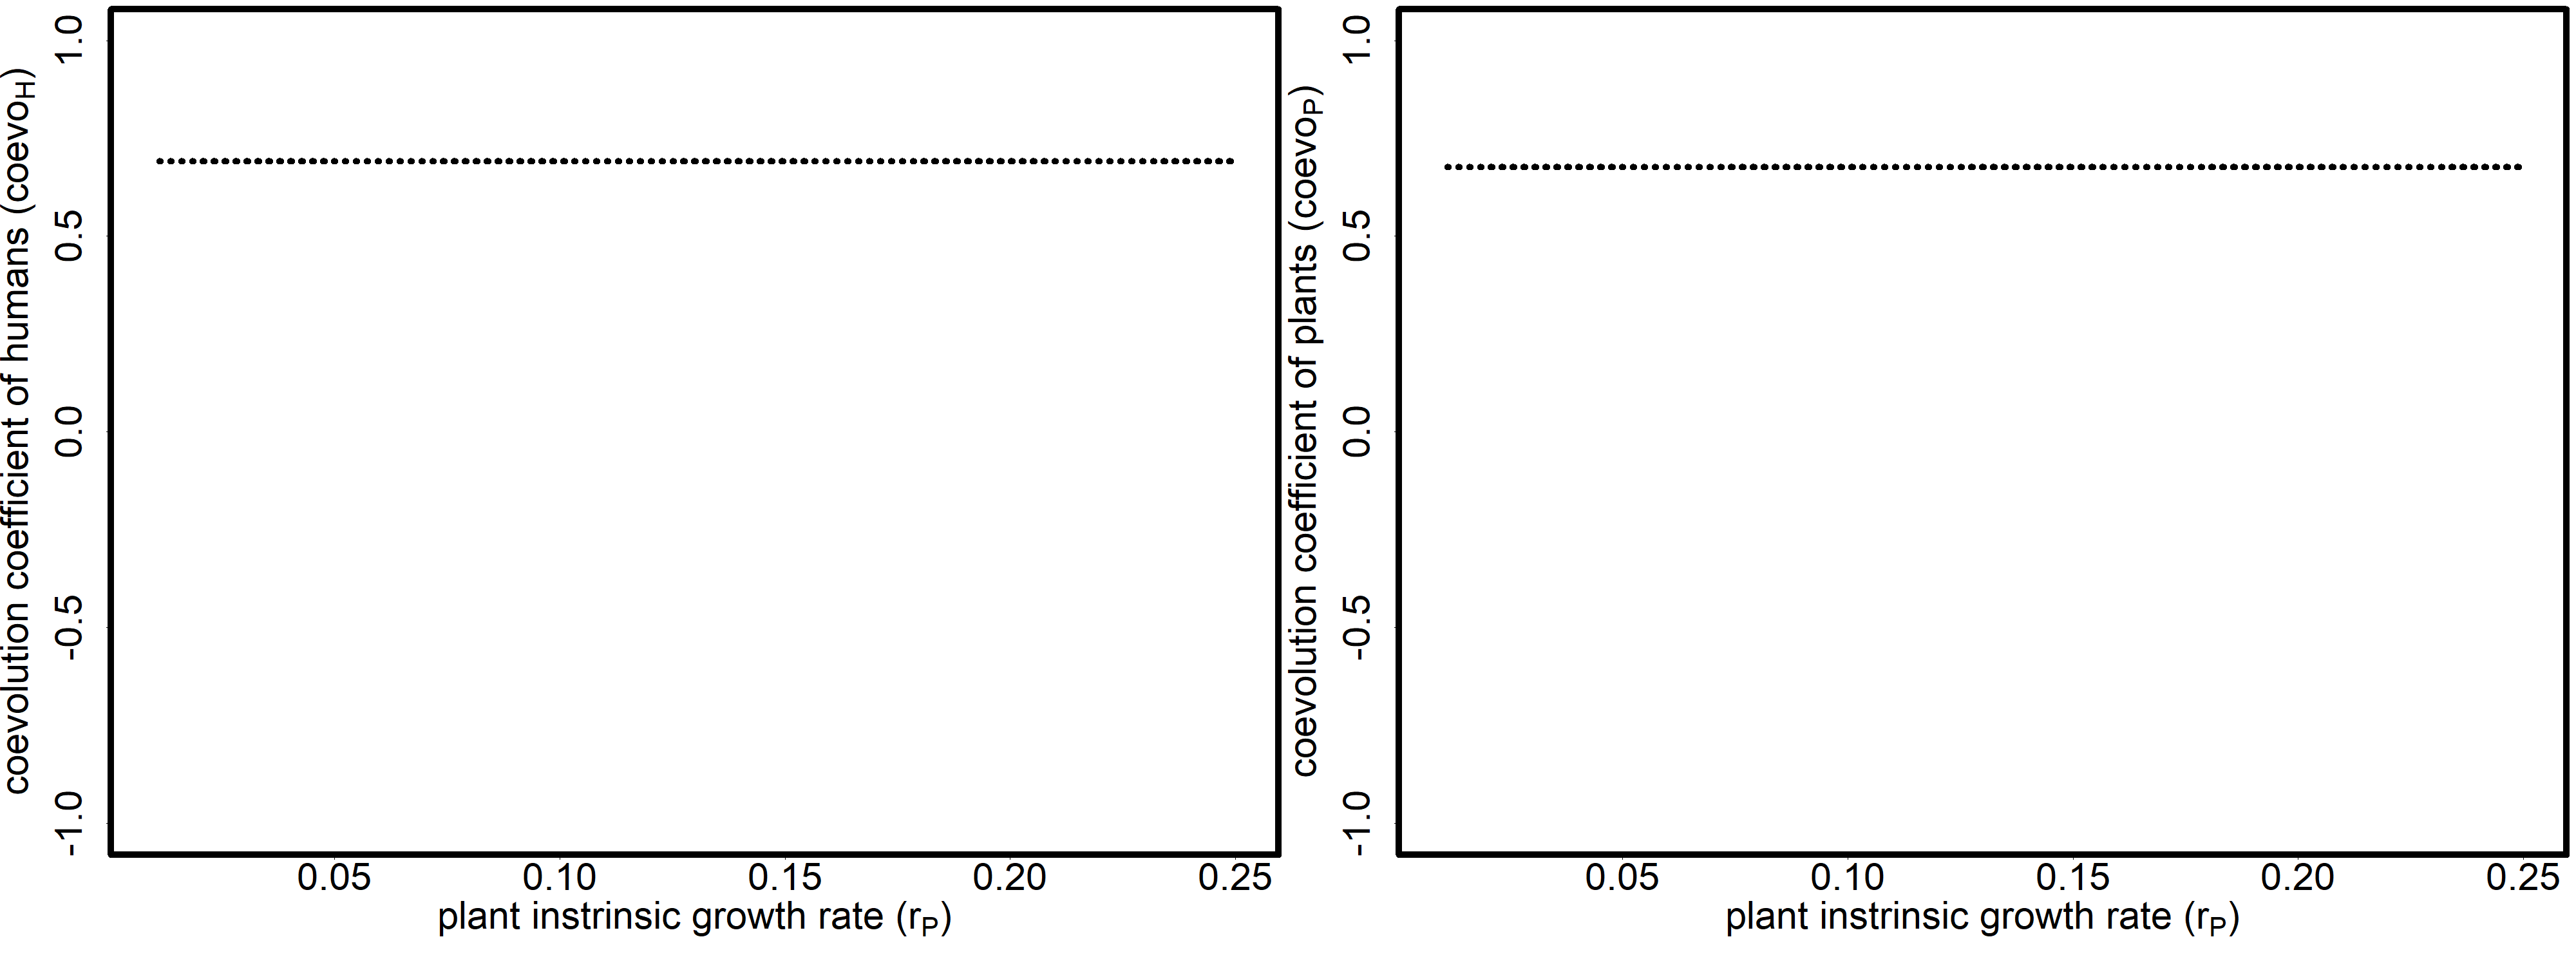
\includegraphics[width=1\linewidth]{plots/2_exp_intrinsic_growth_rate_plants_bifurcationPlotPair}

\hypertarget{utility-per-capita-of-type-n-plants-to-humans-baru_p_nh-1}{%
\subsection{\texorpdfstring{utility per capita \textbf{of} type n plants \textbf{to} humans (\(\bar{U}_{P_{n}H}\)):}{utility per capita of type n plants to humans (\textbackslash bar\{U\}\_\{P\_\{n\}H\}):}}\label{utility-per-capita-of-type-n-plants-to-humans-baru_p_nh-1}}

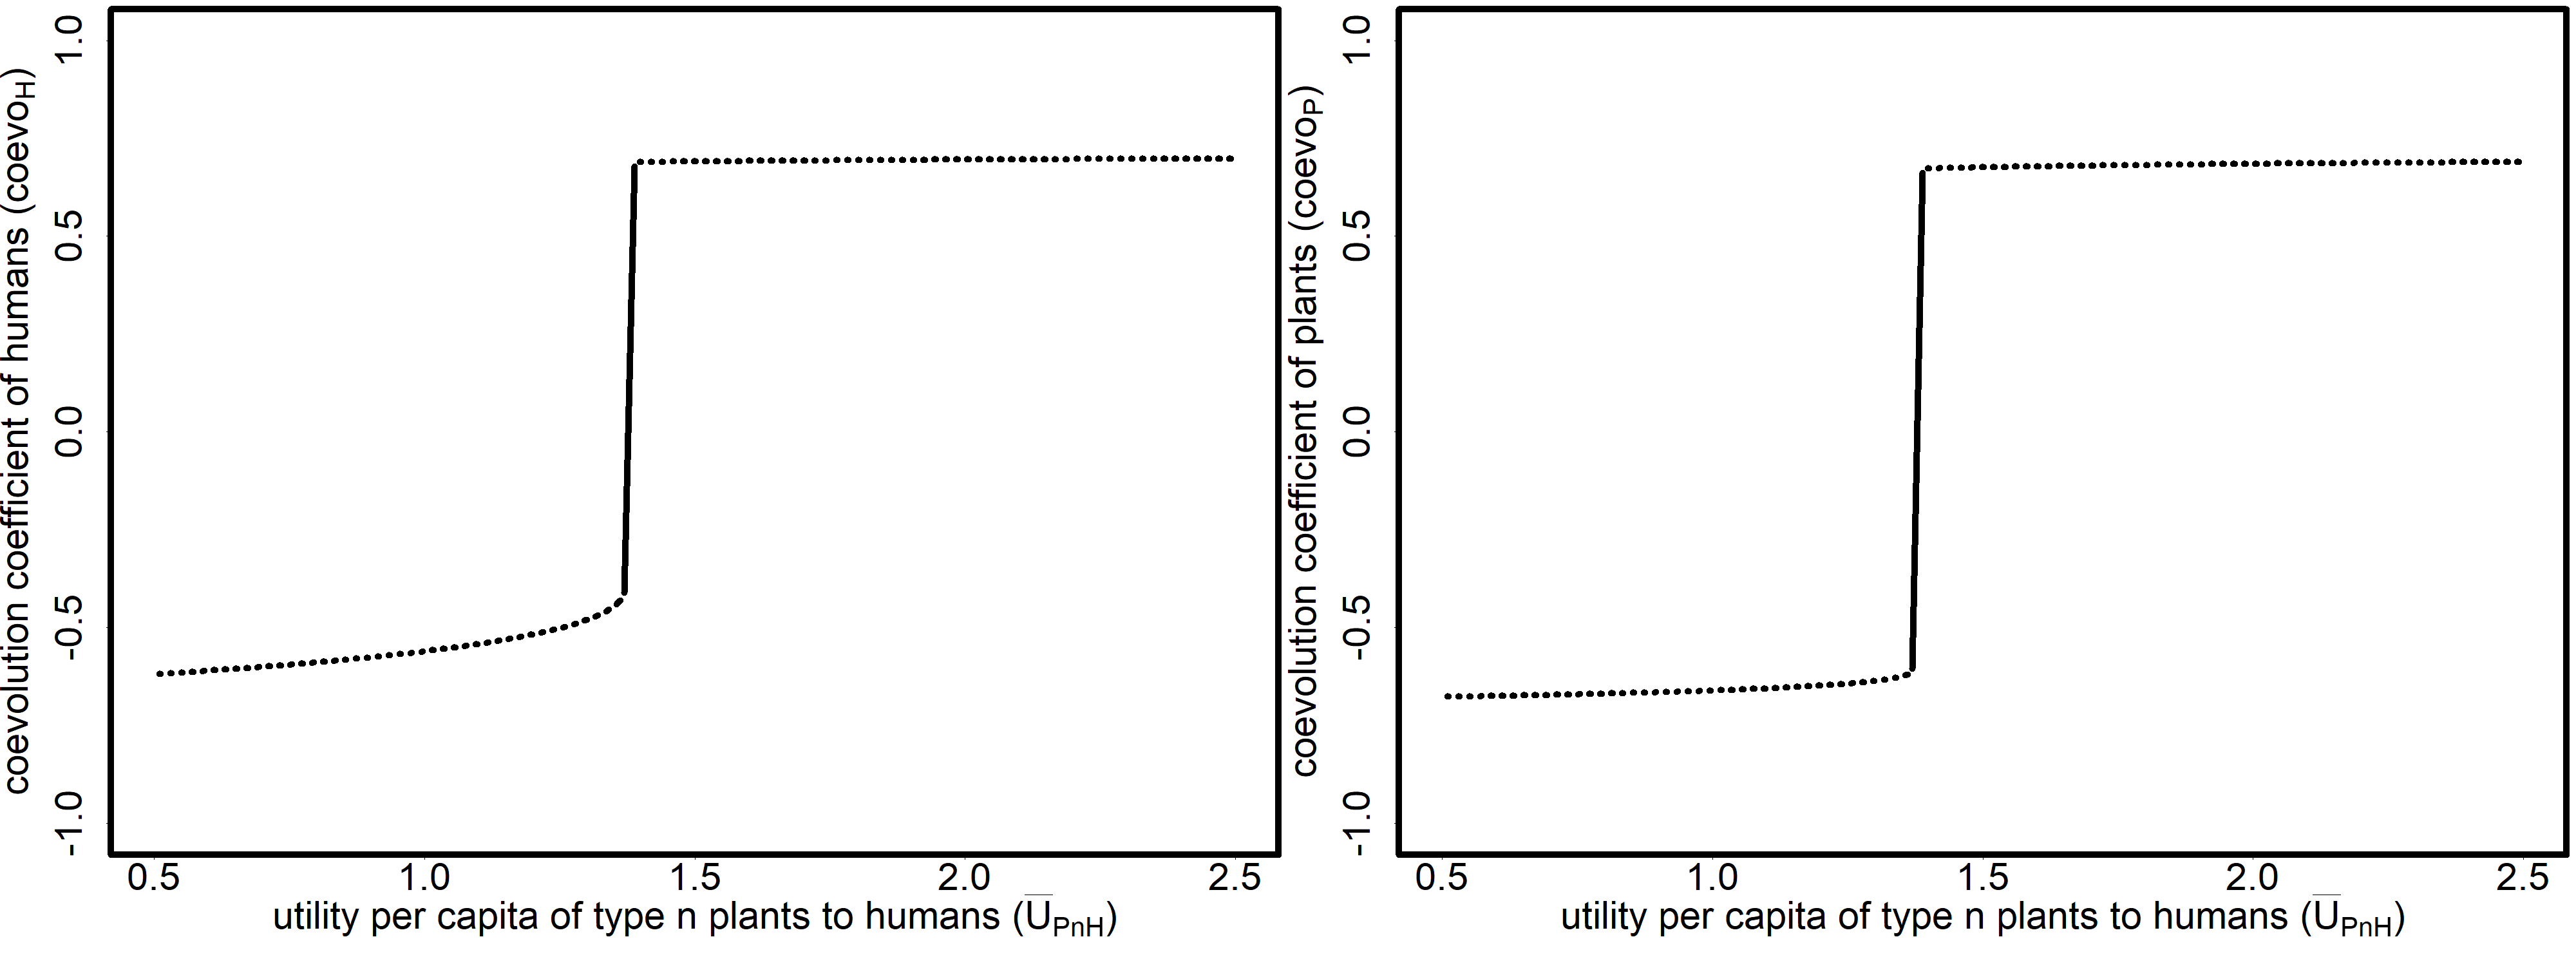
\includegraphics[width=1\linewidth]{plots/2_exp_utility_per_capita_type_n_plants_to_humans_bifurcationPlotPair}

\hypertarget{utility-per-capita-of-type-n-human-to-plants-baru_h_np}{%
\subsection{\texorpdfstring{utility per capita \textbf{of} type n human \textbf{to} plants (\(\bar{U}_{H_{n}P}\)):}{utility per capita of type n human to plants (\textbackslash bar\{U\}\_\{H\_\{n\}P\}):}}\label{utility-per-capita-of-type-n-human-to-plants-baru_h_np}}

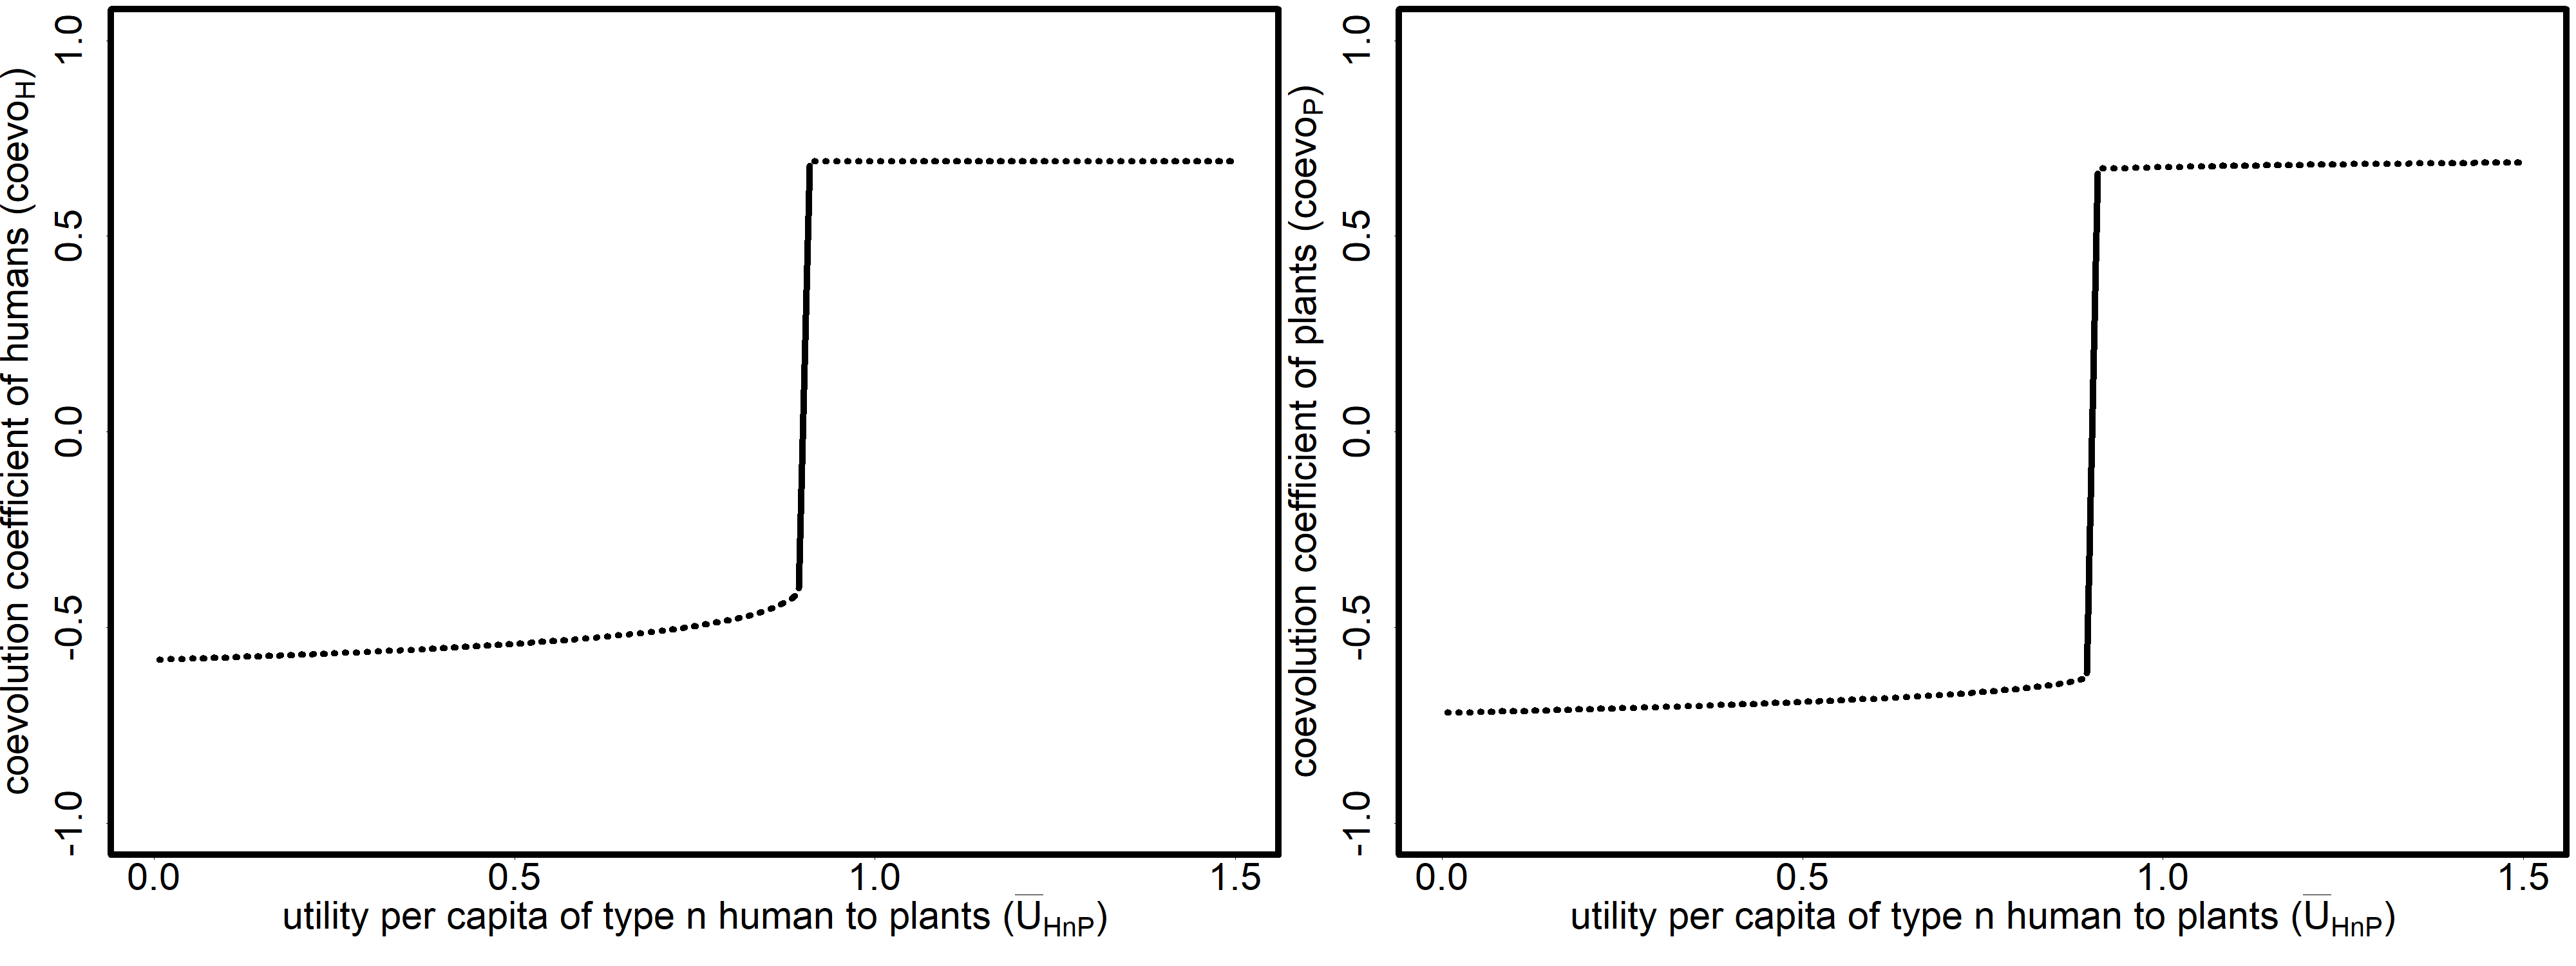
\includegraphics[width=1\linewidth]{plots/2_exp_utility_per_capita_type_n_humans_to_plants_bifurcationPlotPair}

\hypertarget{utility-per-capita-of-type-1-plants-to-humans-baru_p_1h}{%
\subsection{\texorpdfstring{utility per capita \textbf{of} type 1 plants \textbf{to} humans (\(\bar{U}_{P_{1}H}\)):}{utility per capita of type 1 plants to humans (\textbackslash bar\{U\}\_\{P\_\{1\}H\}):}}\label{utility-per-capita-of-type-1-plants-to-humans-baru_p_1h}}

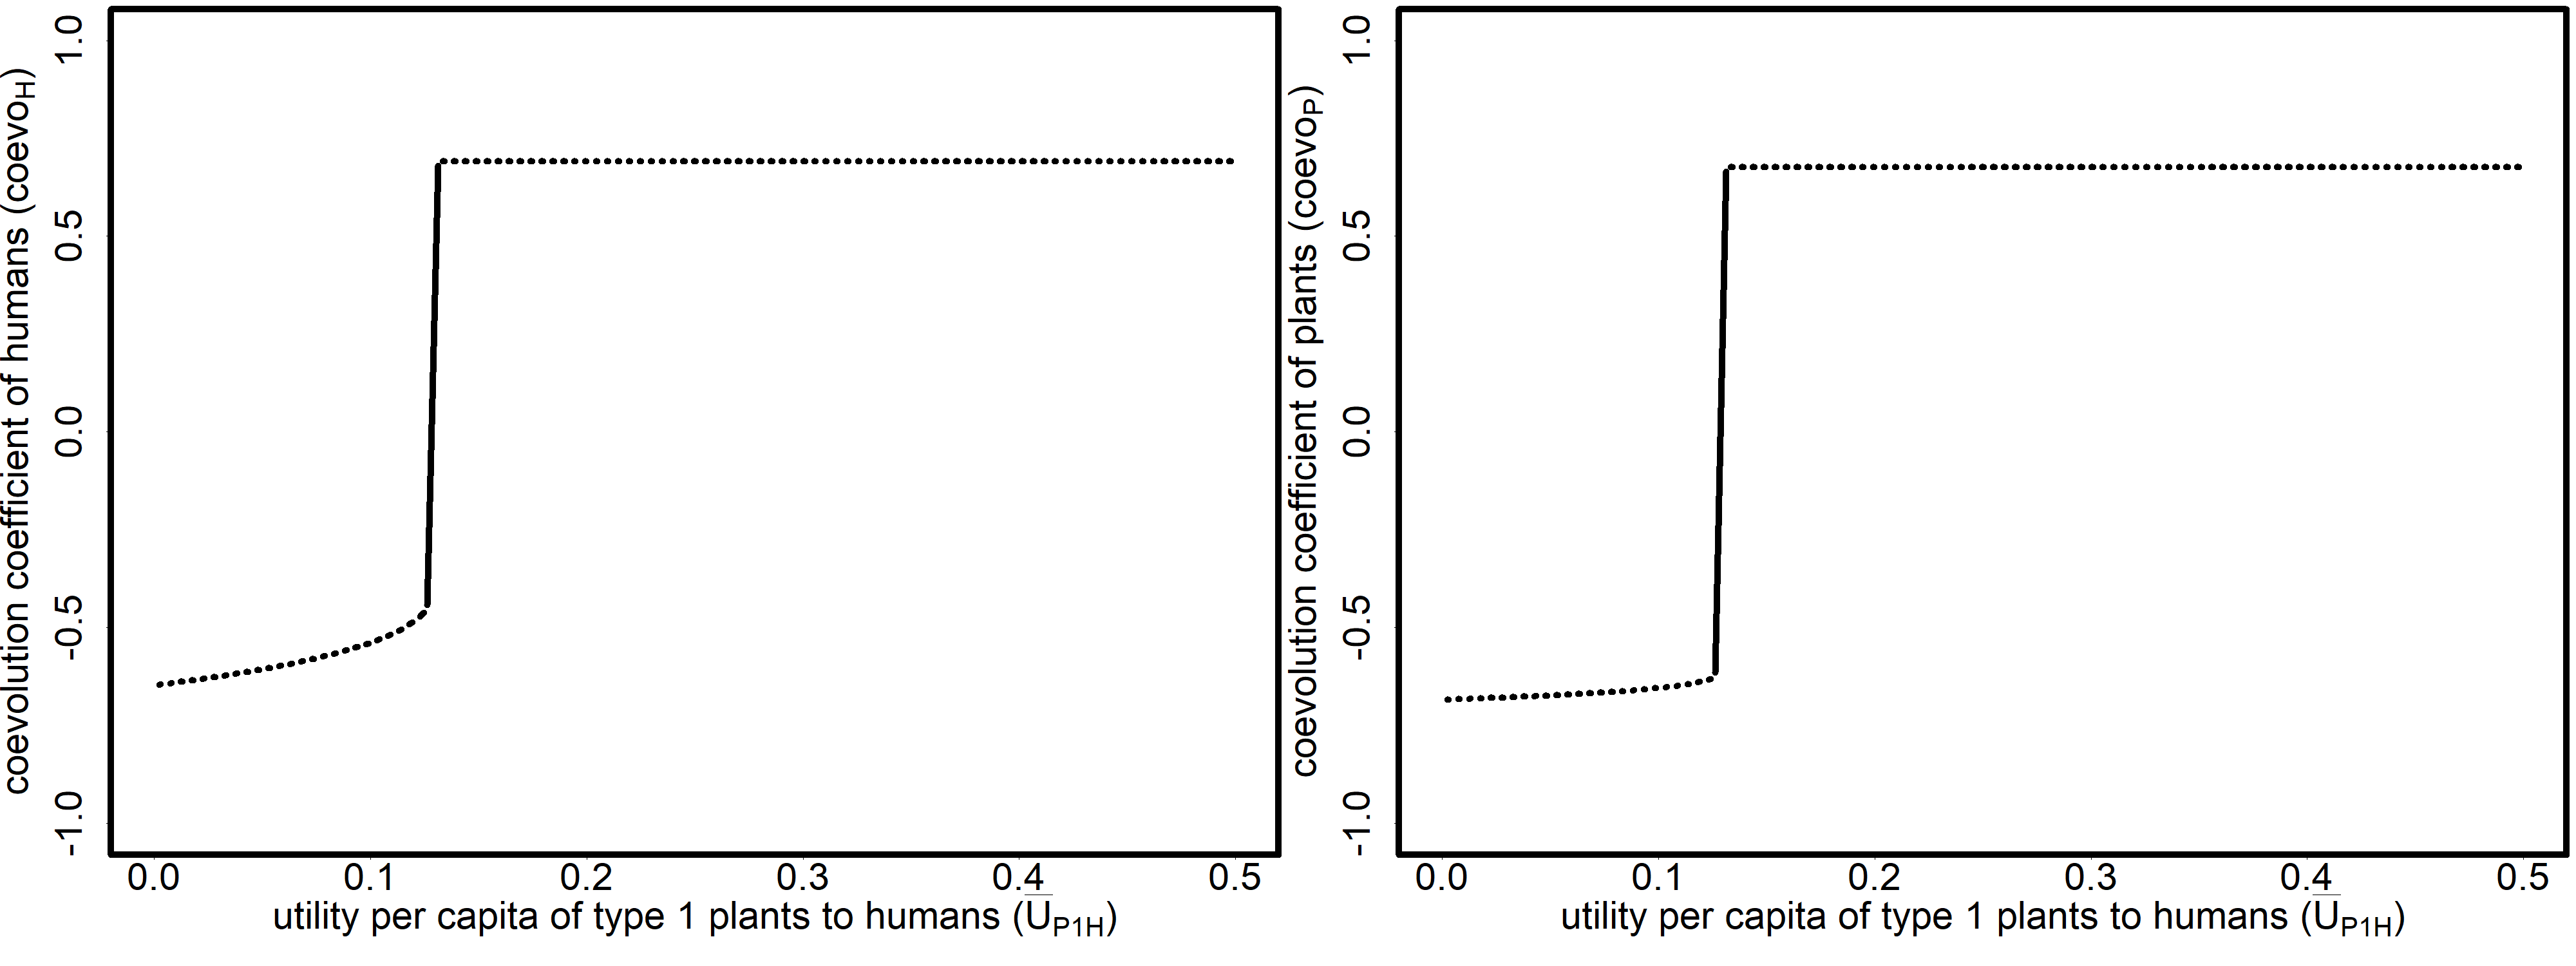
\includegraphics[width=1\linewidth]{plots/2_exp_utility_per_capita_type_1_plants_to_humans_bifurcationPlotPair}

\hypertarget{utility-per-capita-of-type-1-humans-to-plants-baru_h_1p}{%
\subsection{\texorpdfstring{utility per capita \textbf{of} type 1 humans \textbf{to} plants (\(\bar{U}_{H_{1}P}\)):}{utility per capita of type 1 humans to plants (\textbackslash bar\{U\}\_\{H\_\{1\}P\}):}}\label{utility-per-capita-of-type-1-humans-to-plants-baru_h_1p}}

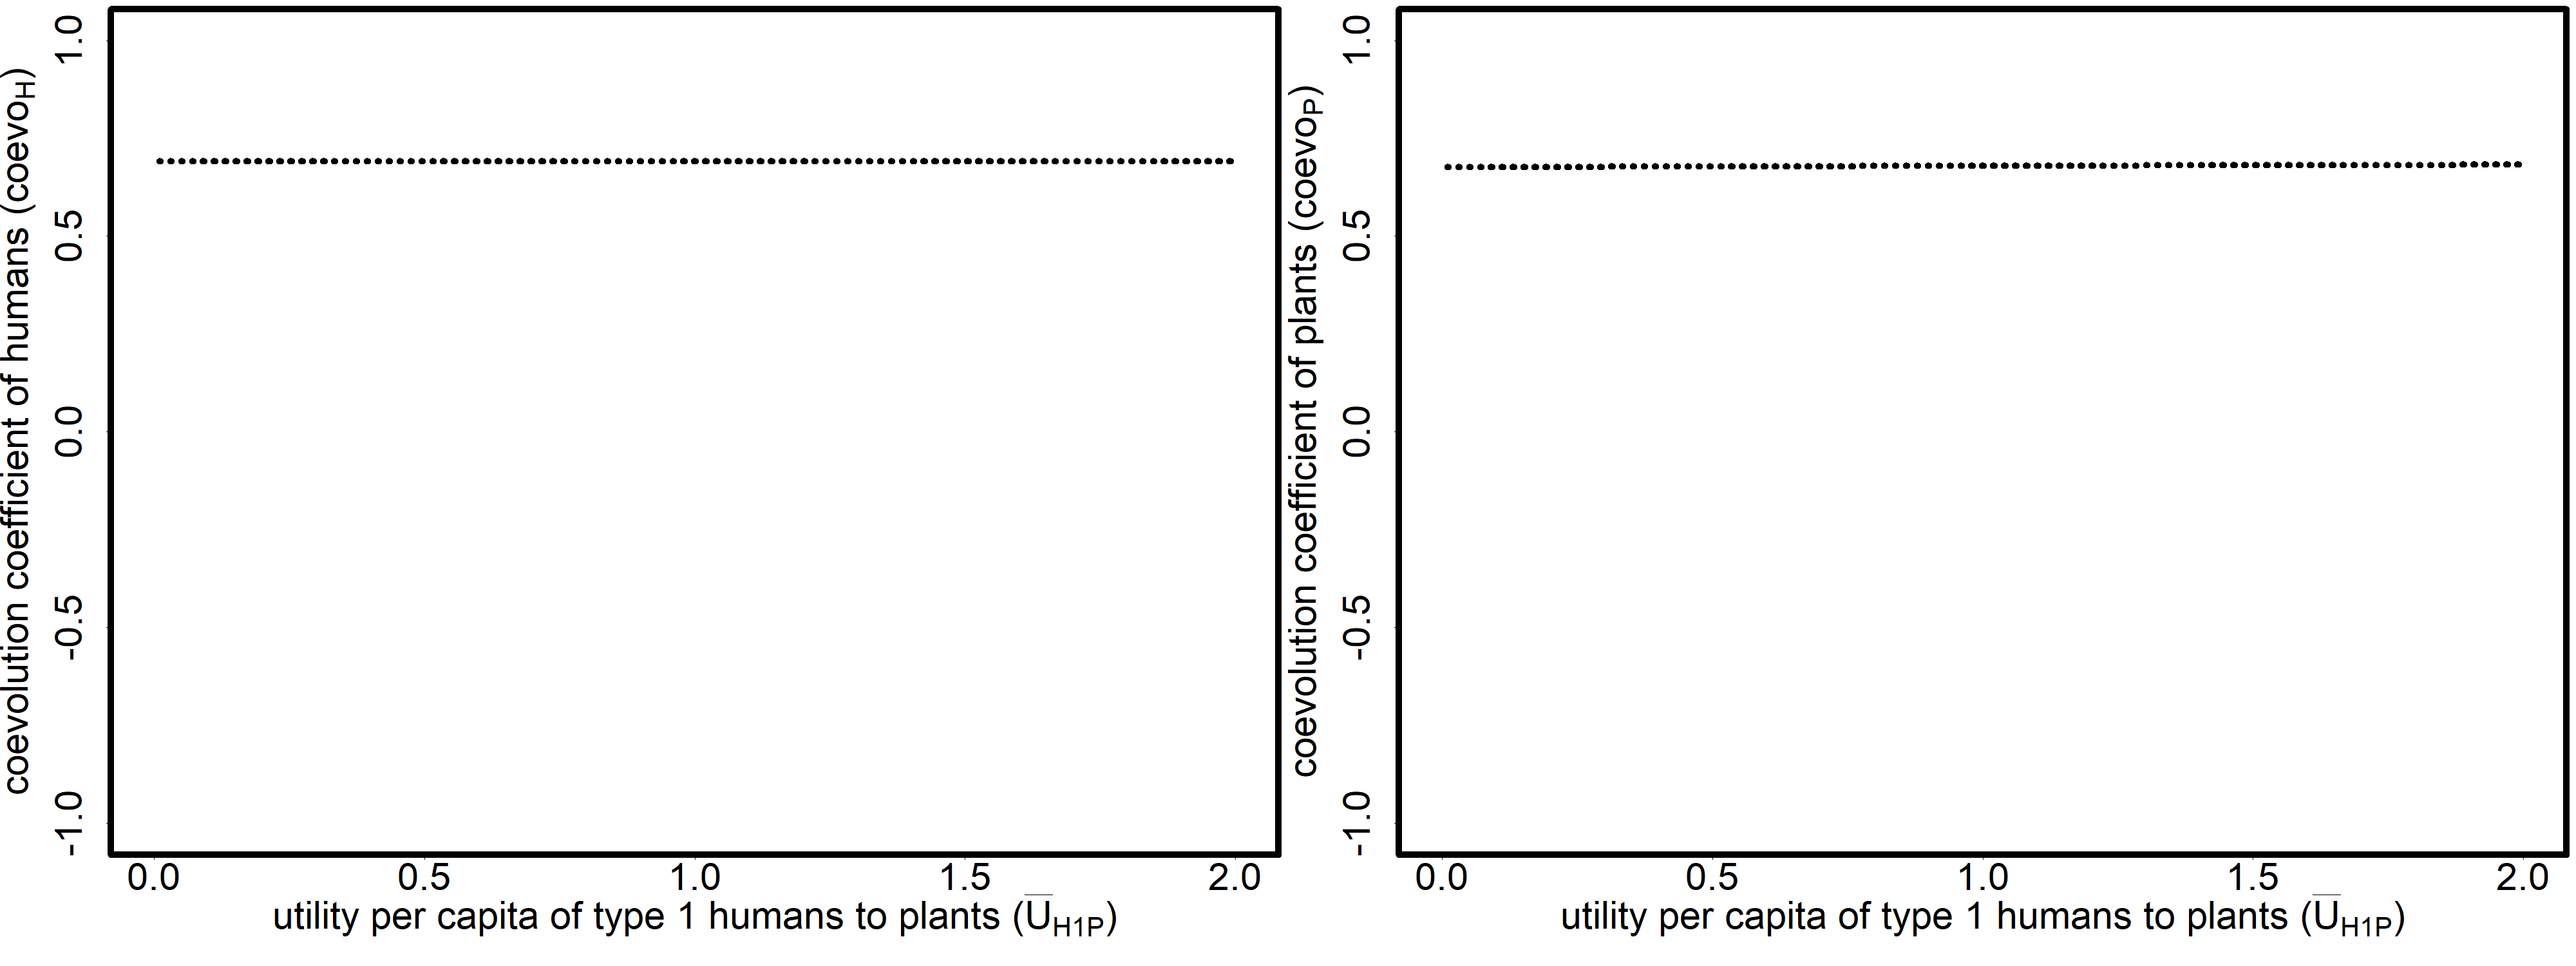
\includegraphics[width=1\linewidth]{plots/2_exp_utility_per_capita_type_1_humans_to_plants_bifurcationPlotPair}

\hypertarget{utility-of-other-resources-to-humans-of-type-1-u_bh_1}{%
\subsection{\texorpdfstring{utility \textbf{of} other resources \textbf{to} humans of type 1 (\(U_{bH_{1}}\)):}{utility of other resources to humans of type 1 (U\_\{bH\_\{1\}\}):}}\label{utility-of-other-resources-to-humans-of-type-1-u_bh_1}}

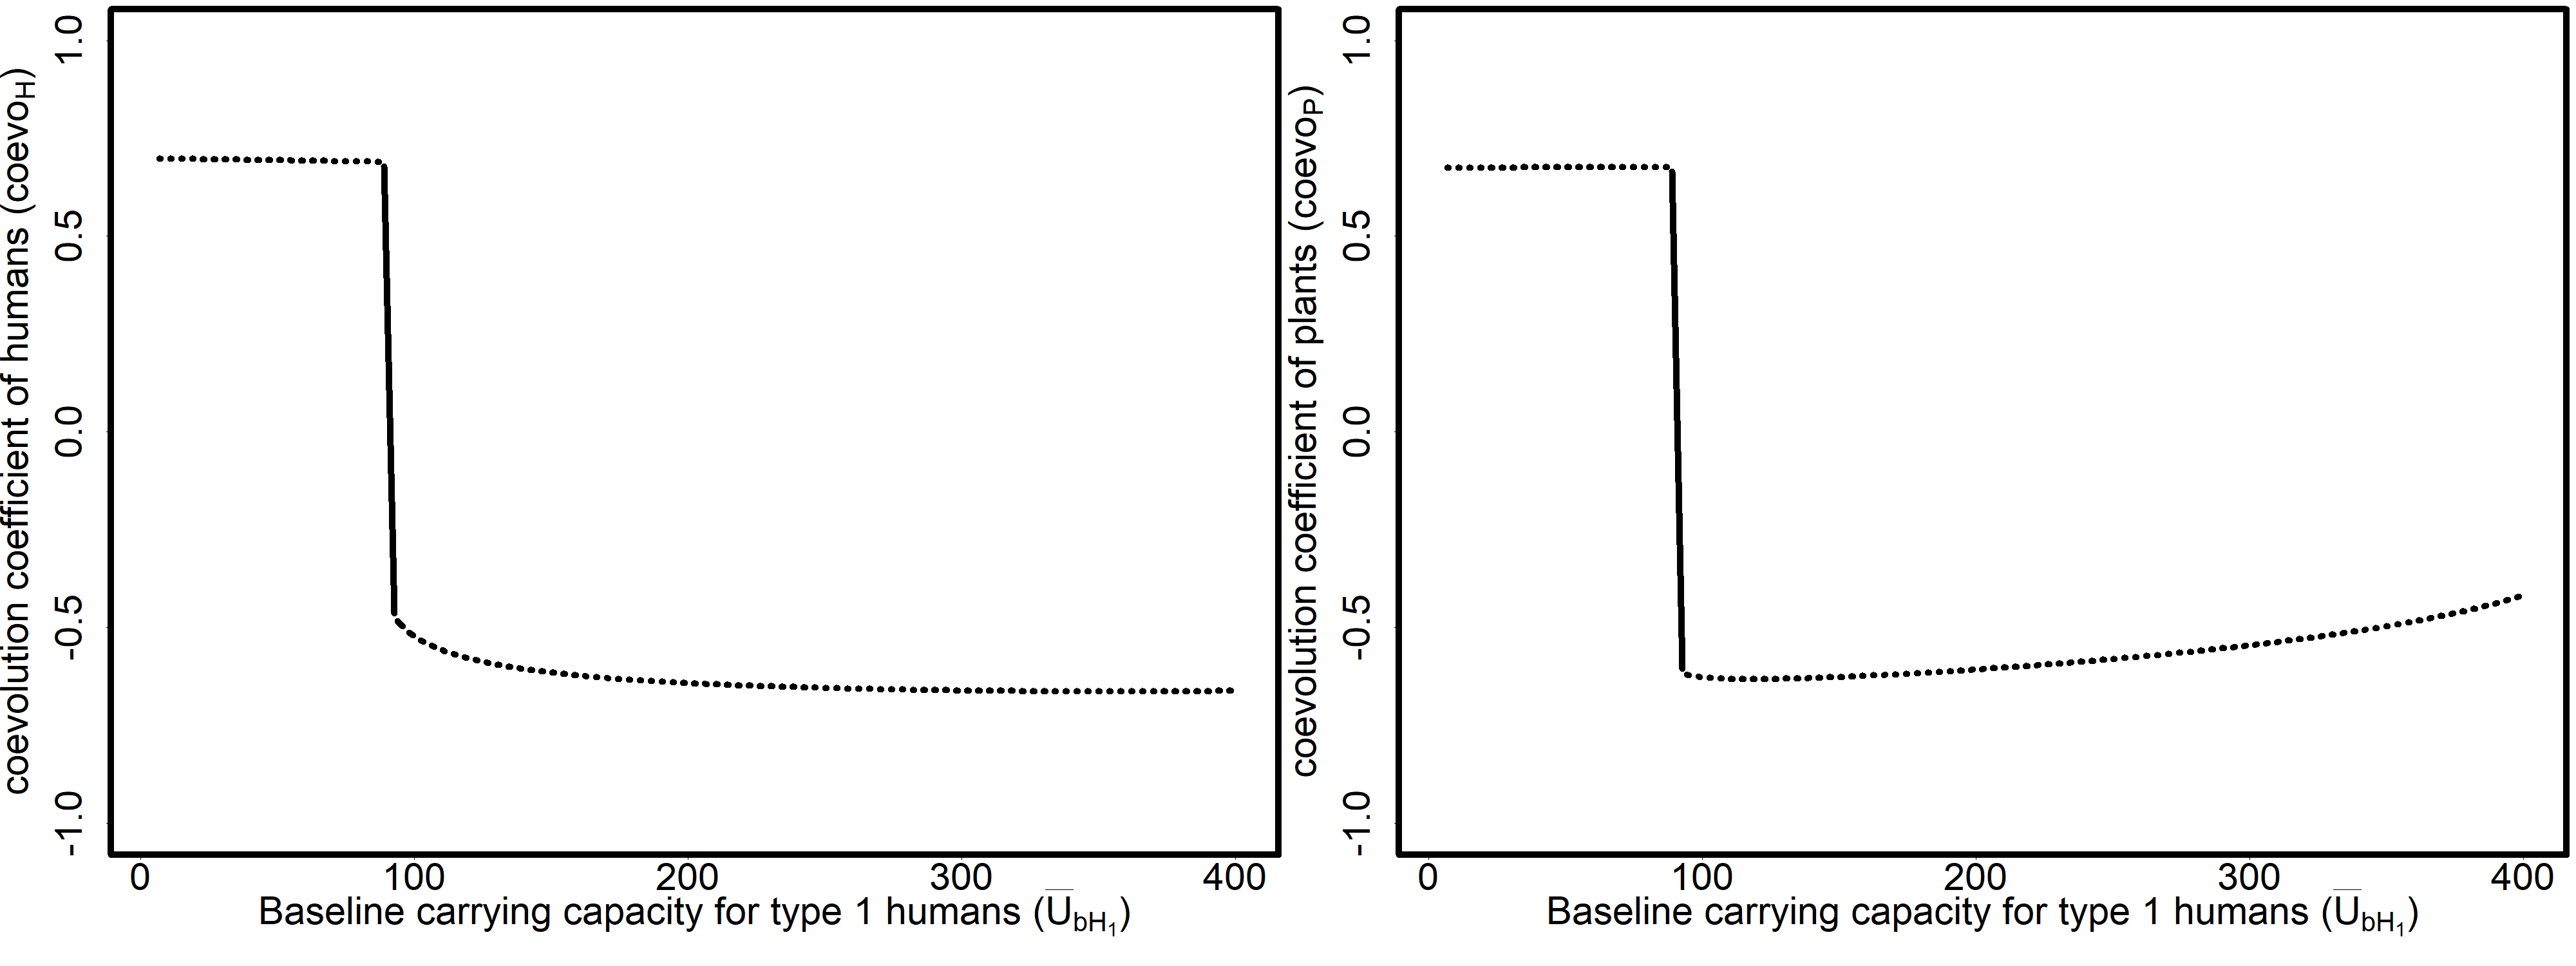
\includegraphics[width=1\linewidth]{plots/2_exp_utility_other_to_type_1_humans_bifurcationPlotPair}

\hypertarget{utility-of-non-anthropic-space-to-type-1-plants-u_bp_1}{%
\subsection{\texorpdfstring{utility \textbf{of} non-anthropic space \textbf{to} type 1 plants (\(U_{bP_{1}}\)):}{utility of non-anthropic space to type 1 plants (U\_\{bP\_\{1\}\}):}}\label{utility-of-non-anthropic-space-to-type-1-plants-u_bp_1}}

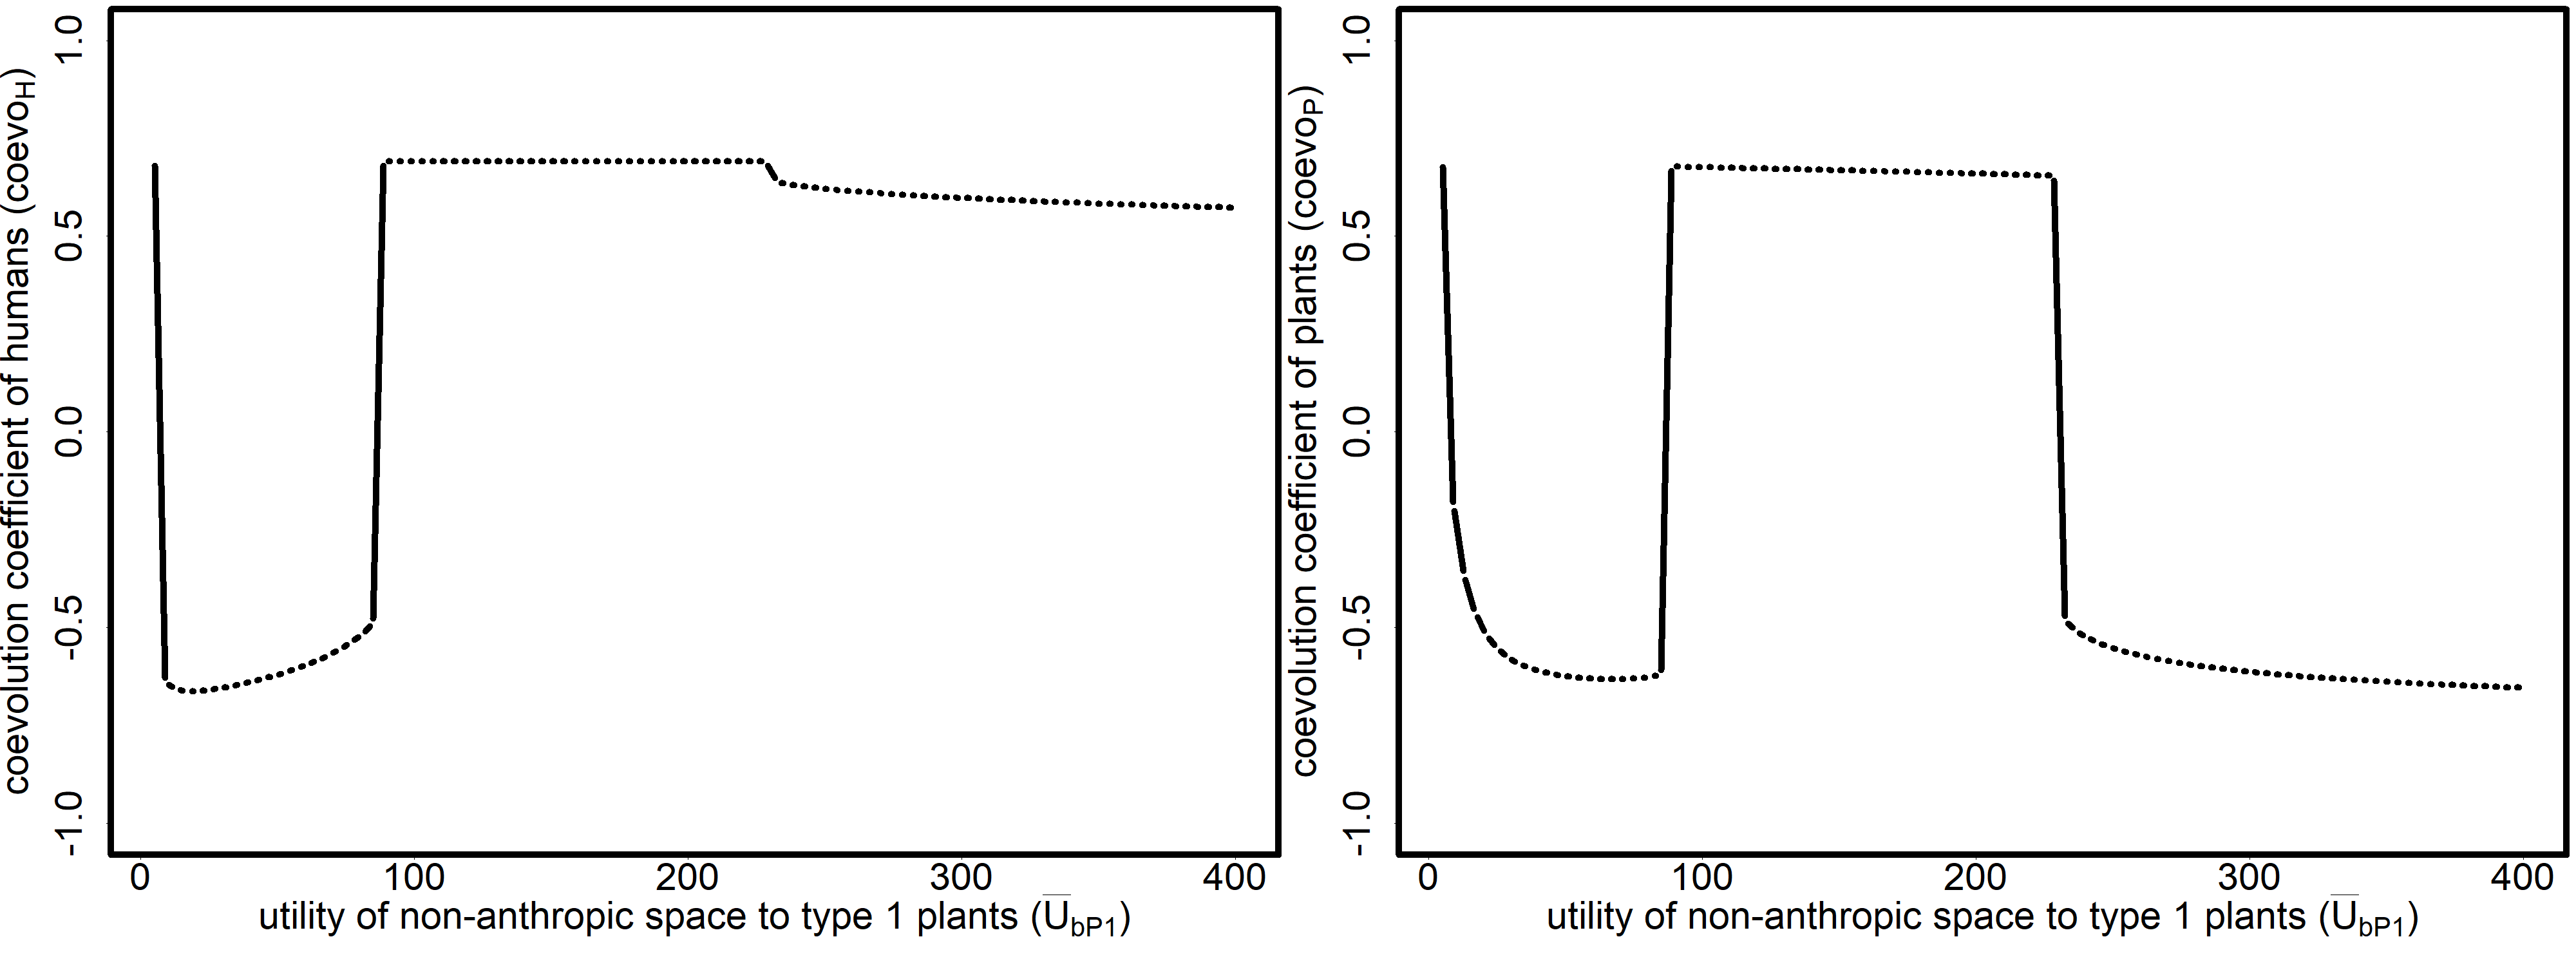
\includegraphics[width=1\linewidth]{plots/2_exp_utility_other_to_type_1_plants_bifurcationPlotPair}

\hypertarget{utility-of-other-resources-to-type-n-humans-u_bh_n}{%
\subsection{\texorpdfstring{utility \textbf{of} other resources \textbf{to} type n humans (\(U_{bH_{n}}\)):}{utility of other resources to type n humans (U\_\{bH\_\{n\}\}):}}\label{utility-of-other-resources-to-type-n-humans-u_bh_n}}

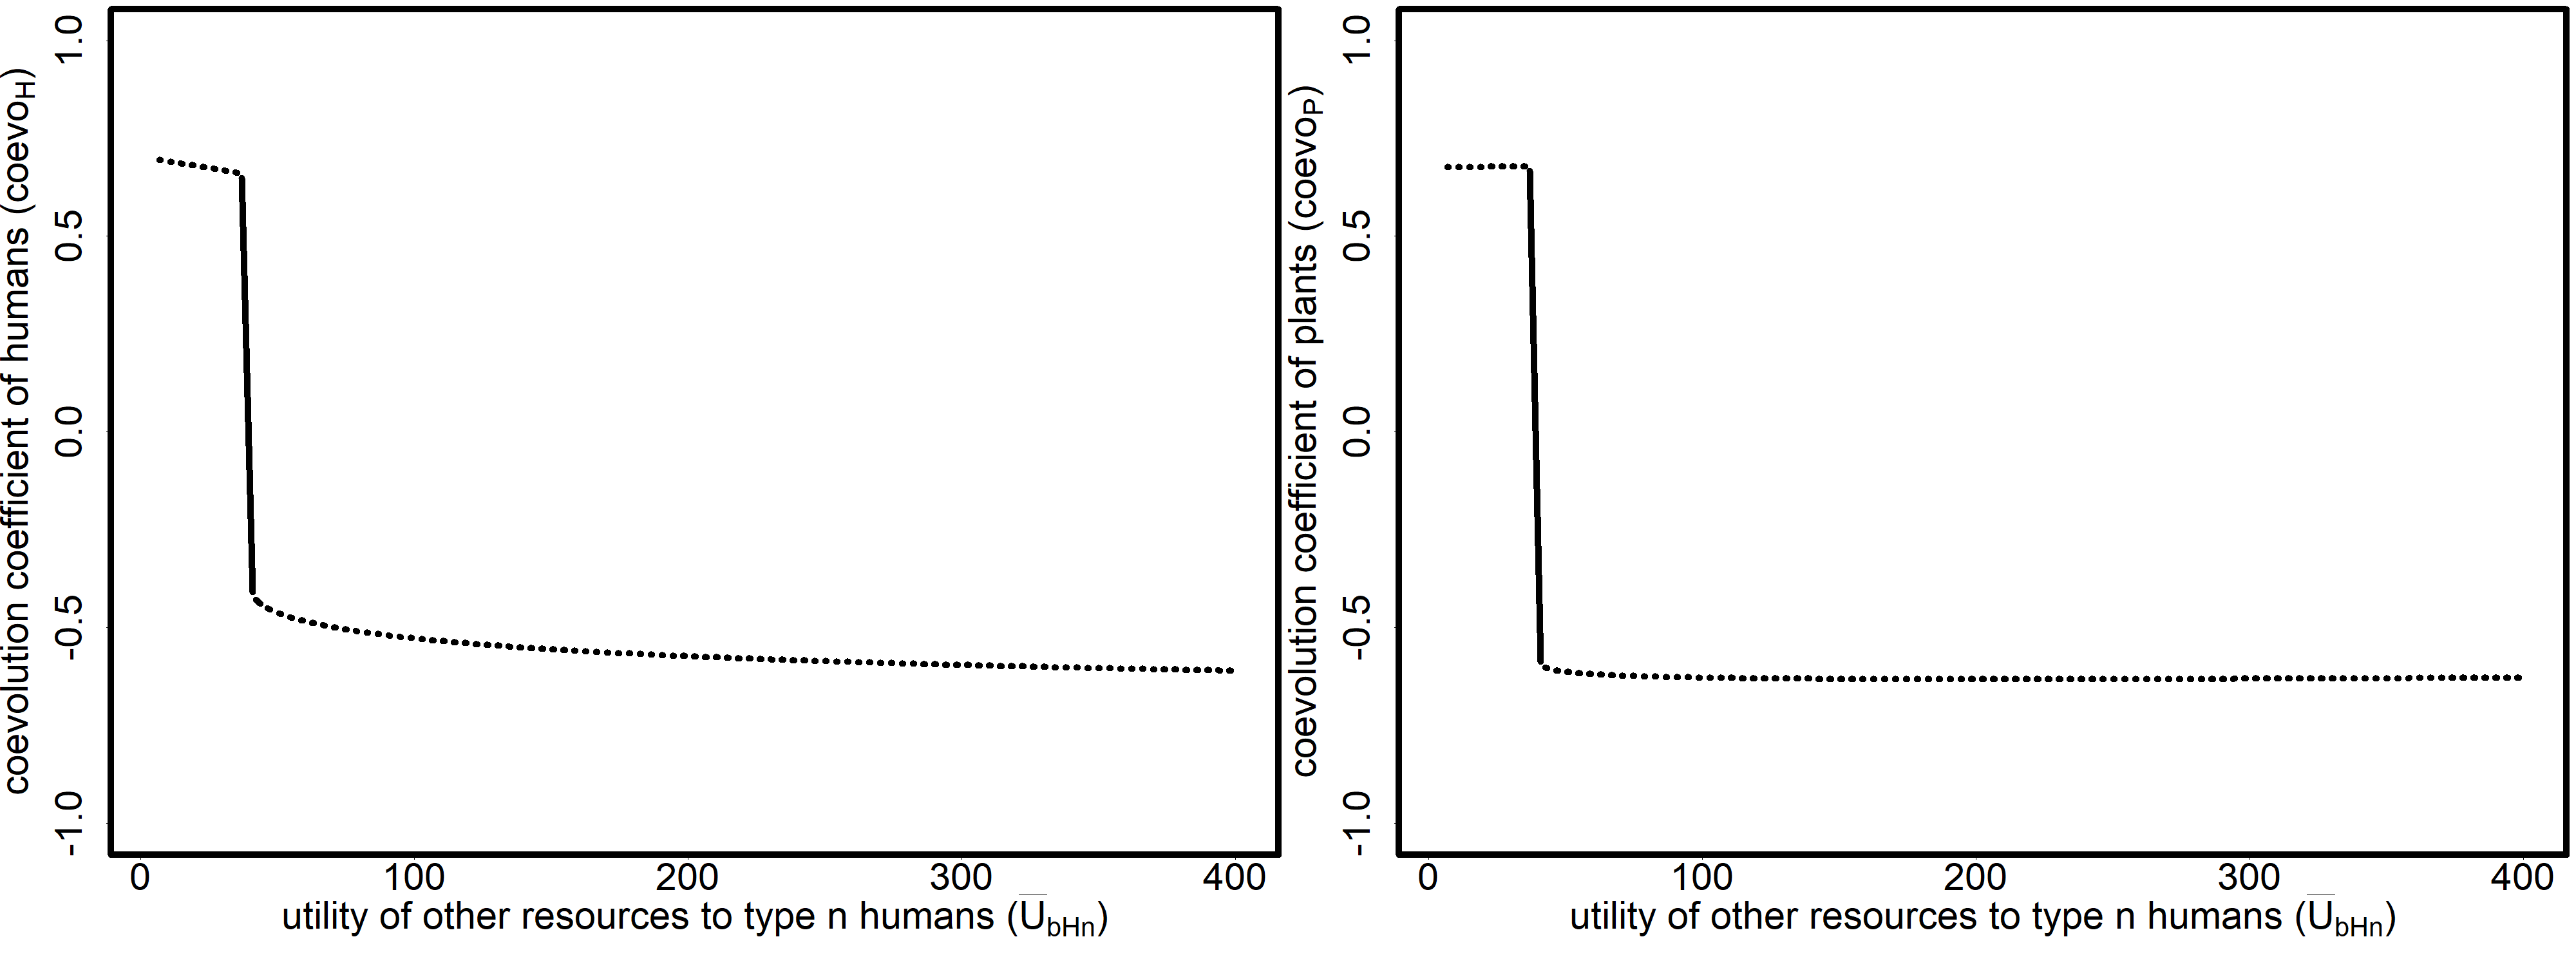
\includegraphics[width=1\linewidth]{plots/2_exp_utility_other_to_type_n_humans_bifurcationPlotPair}

\hypertarget{utility-of-non-anthropic-space-to-type-n-plants-u_bp_n}{%
\subsection{\texorpdfstring{utility \textbf{of} non-anthropic space \textbf{to} type n plants (\(U_{bP_{n}}\)):}{utility of non-anthropic space to type n plants (U\_\{bP\_\{n\}\}):}}\label{utility-of-non-anthropic-space-to-type-n-plants-u_bp_n}}

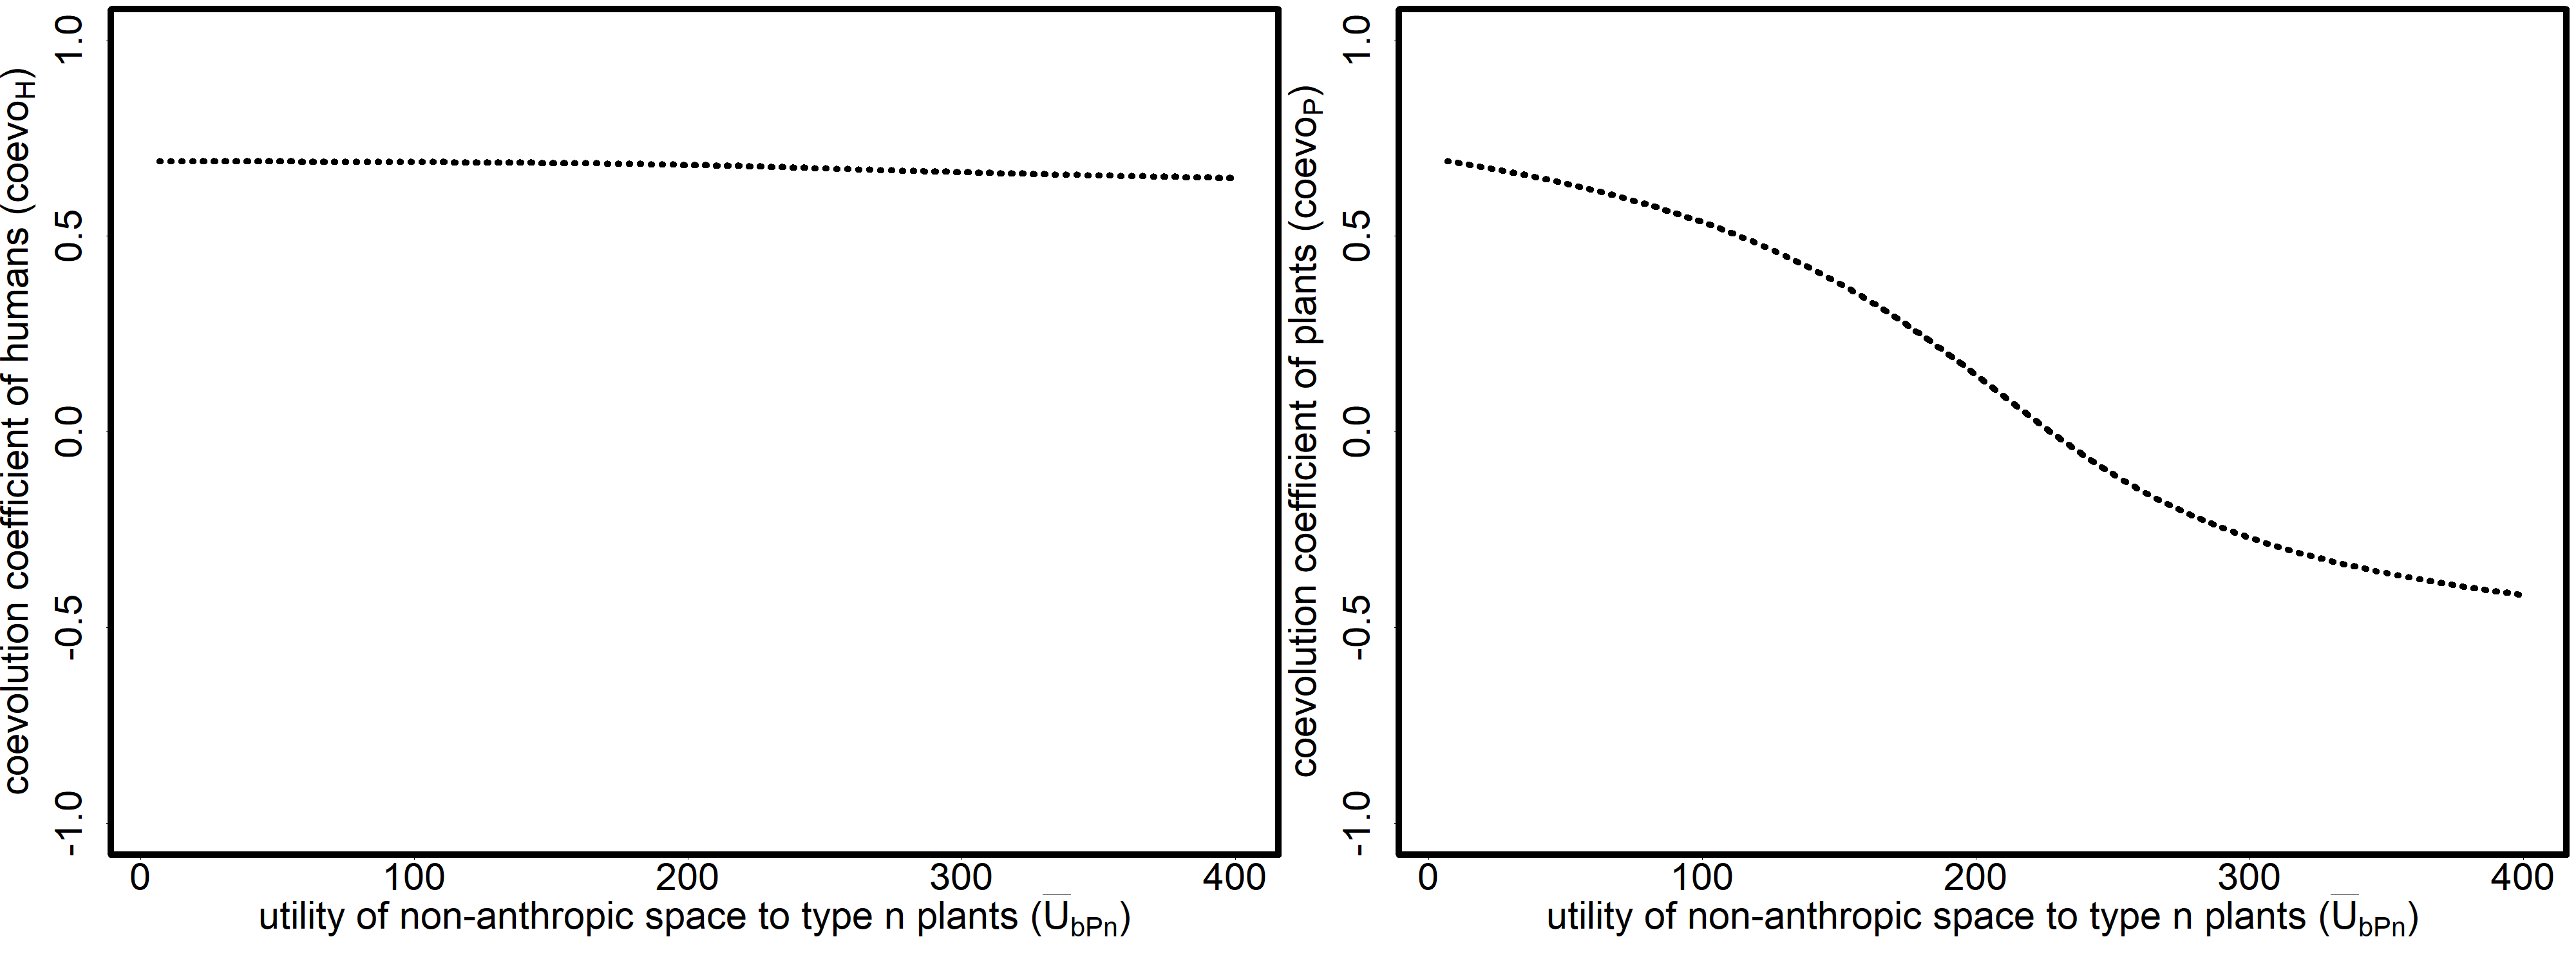
\includegraphics[width=1\linewidth]{plots/2_exp_utility_other_to_type_n_plants_bifurcationPlotPair}

\hypertarget{maximum-contiguous-area-to-be-used-by-plants-max_area}{%
\subsection{\texorpdfstring{maximum contiguous area to be used by plants (\(max_area\)):}{maximum contiguous area to be used by plants (max\_area):}}\label{maximum-contiguous-area-to-be-used-by-plants-max_area}}

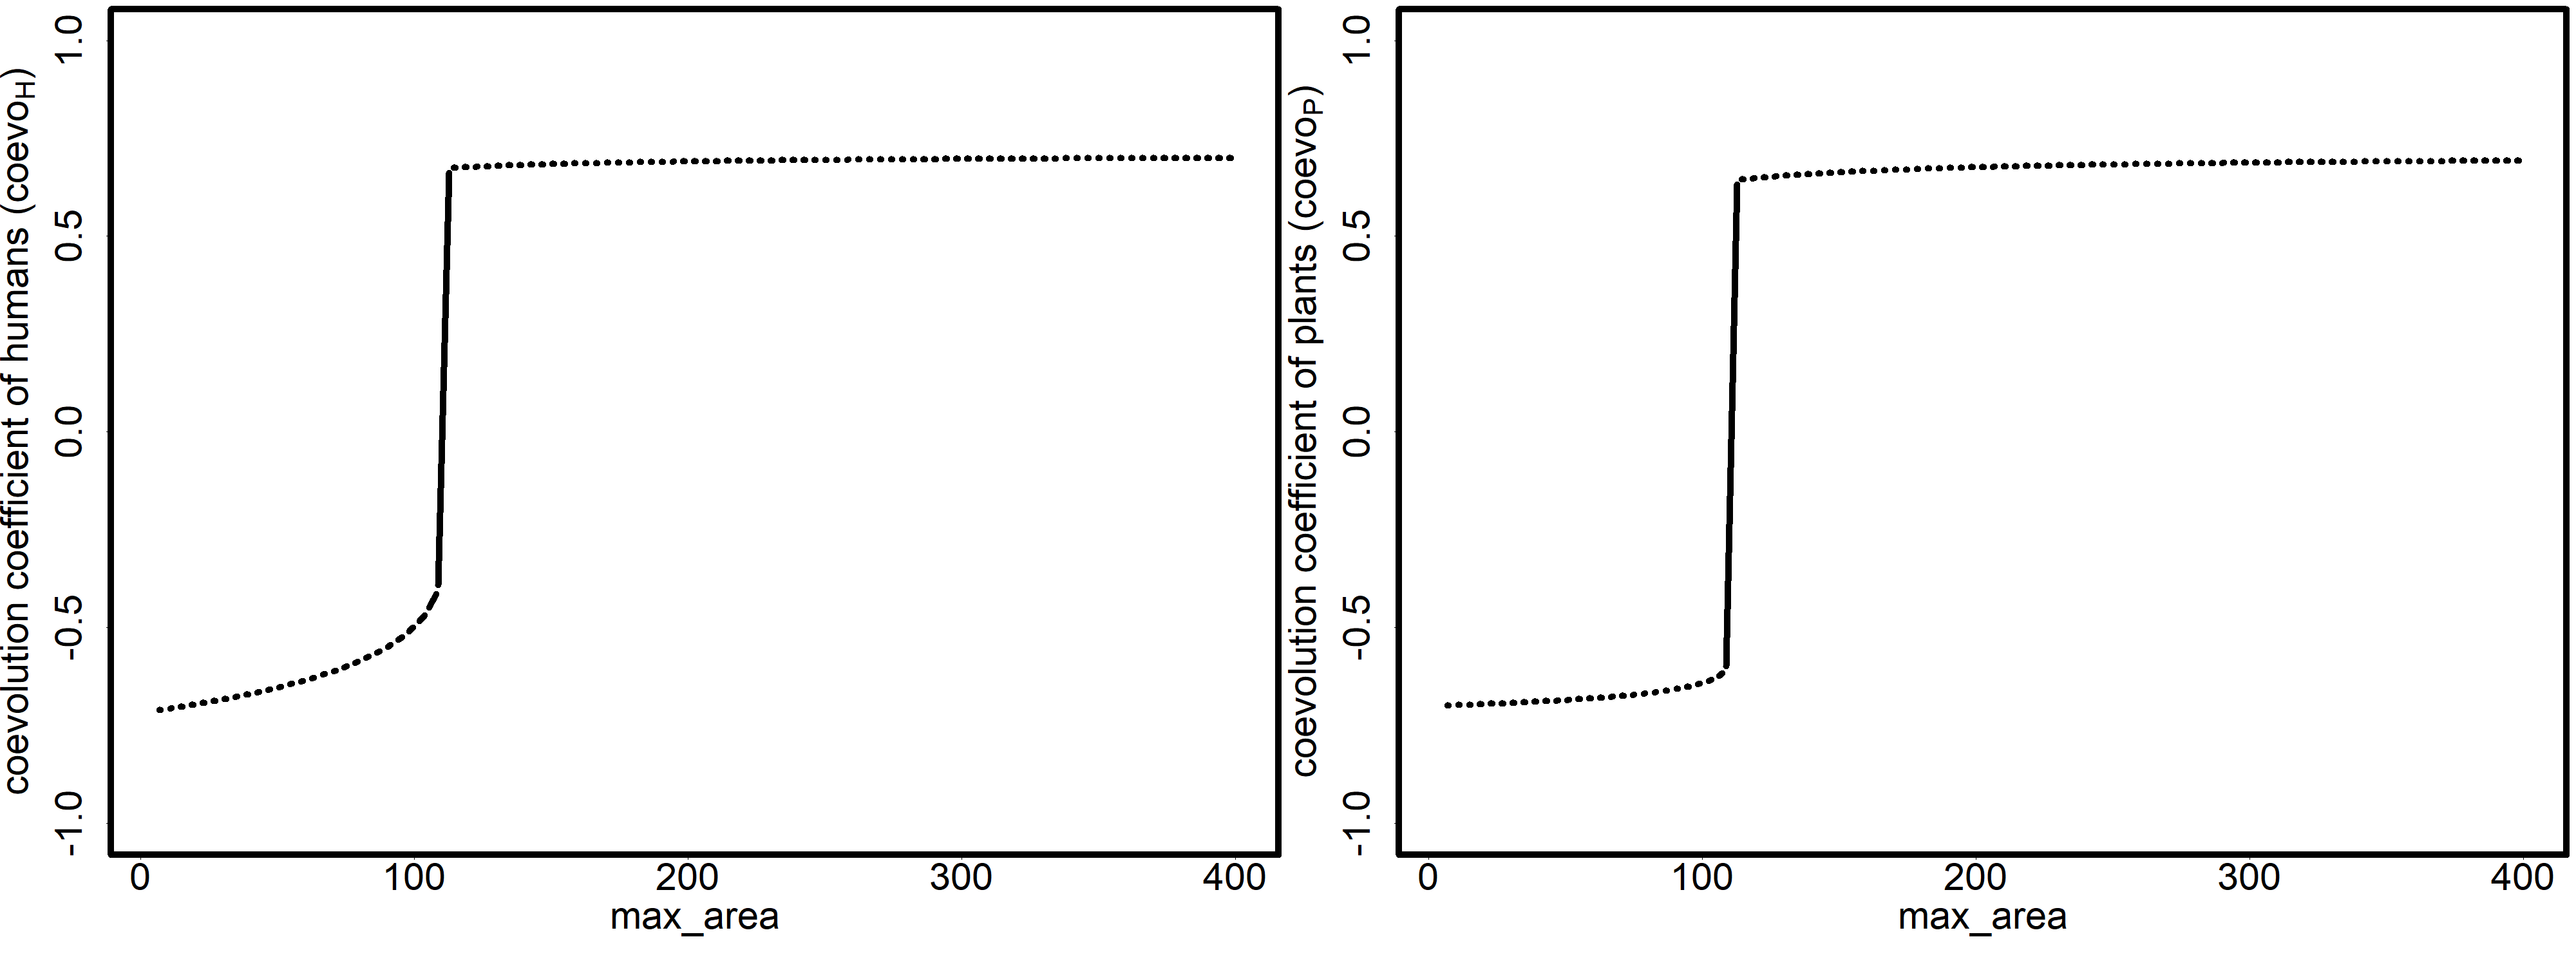
\includegraphics[width=1\linewidth]{plots/2_exp_max_area_bifurcationPlotPair}

\begin{center}\rule{0.5\linewidth}{0.5pt}\end{center}

\hypertarget{oscilations}{%
\section{Oscilations}\label{oscilations}}

Bifurcation plot with last 100 time steps (of 1000) to capture oscillations or `slow' asymptotic stability

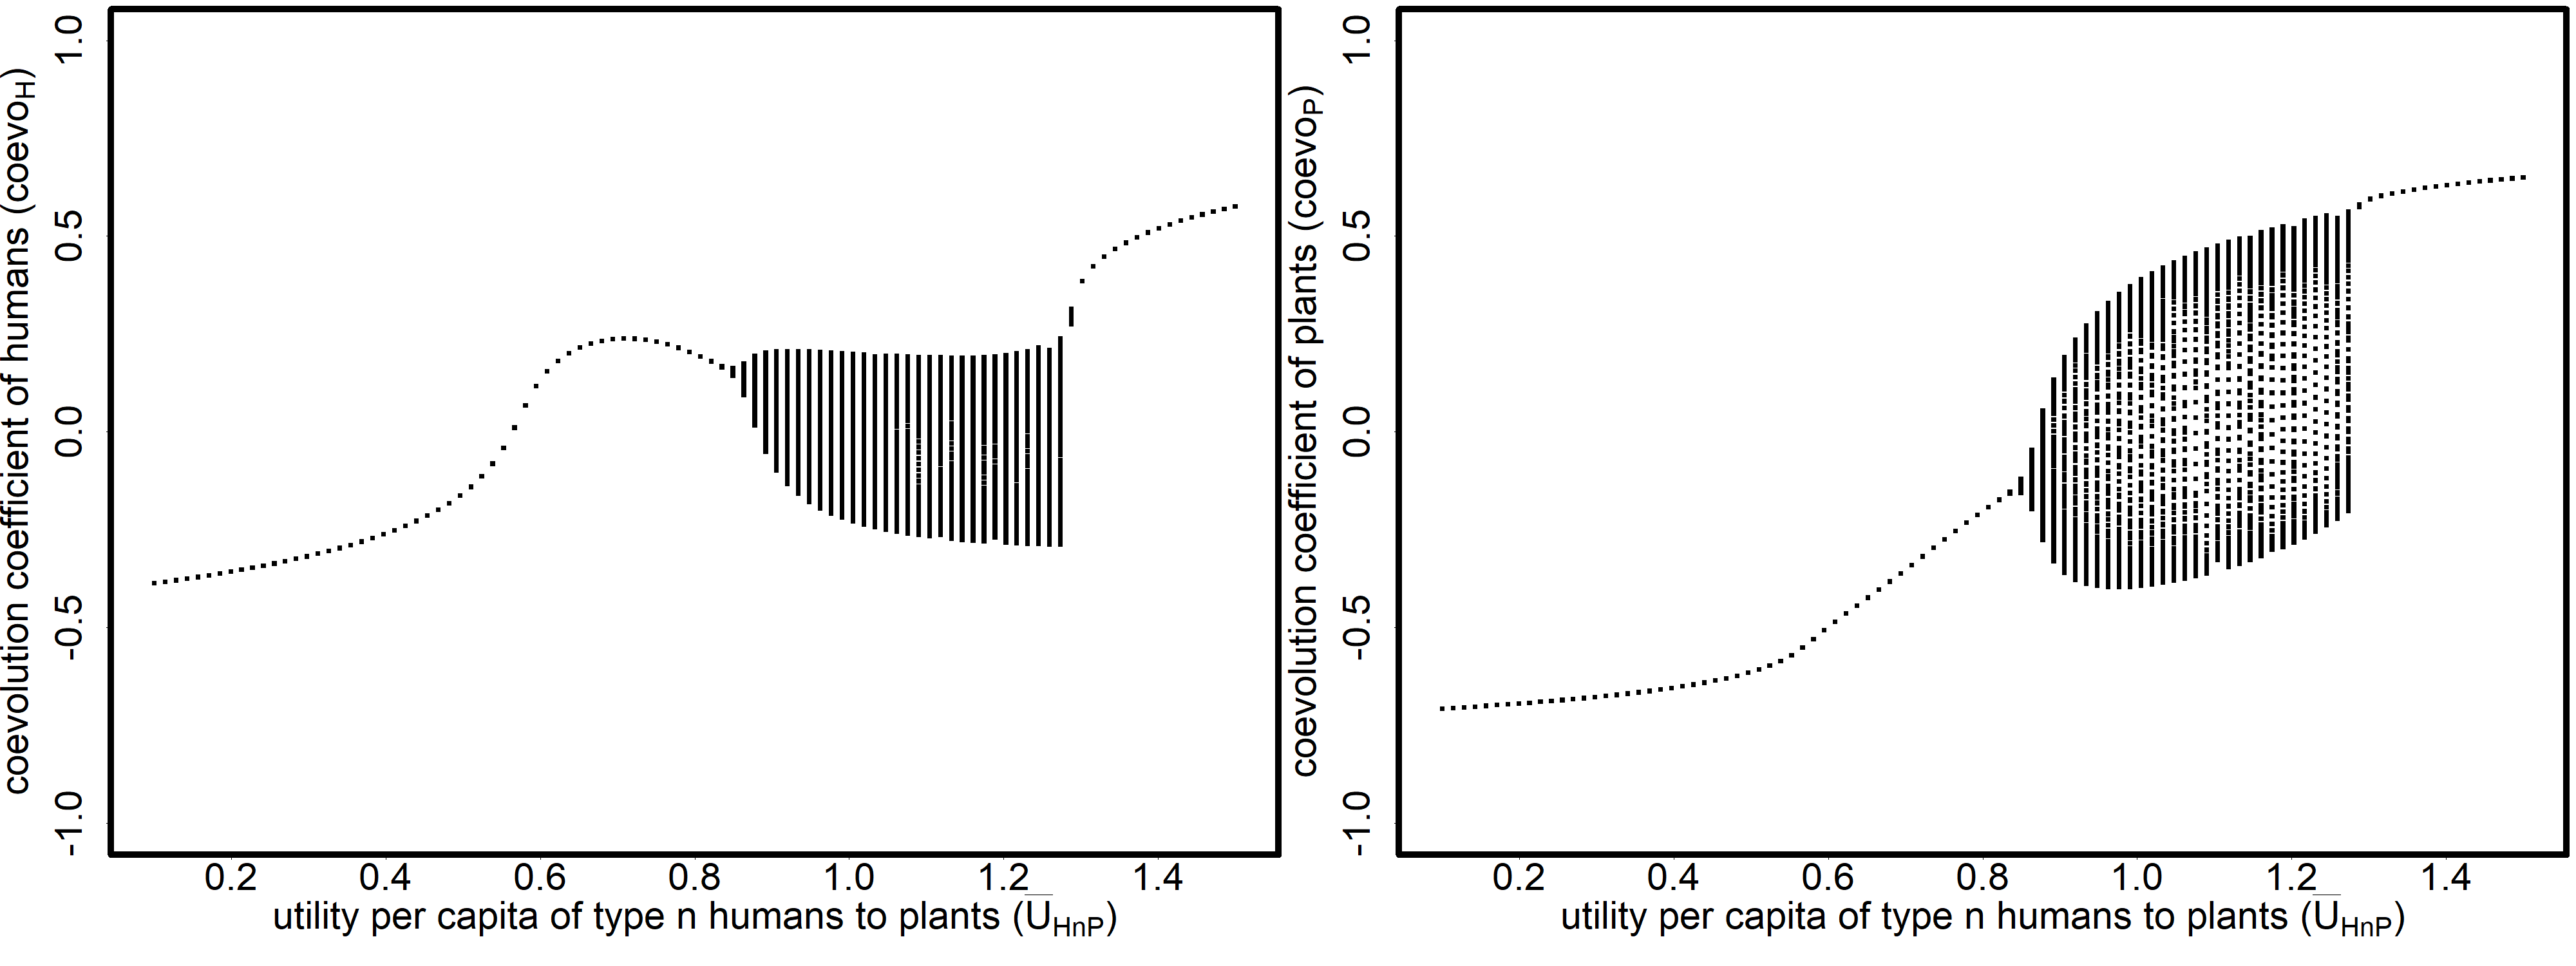
\includegraphics[width=1\linewidth]{plots/2_exp_utility_per_capita_type_n_humans_to_plants_oscillation_bifurcationPlotPair}

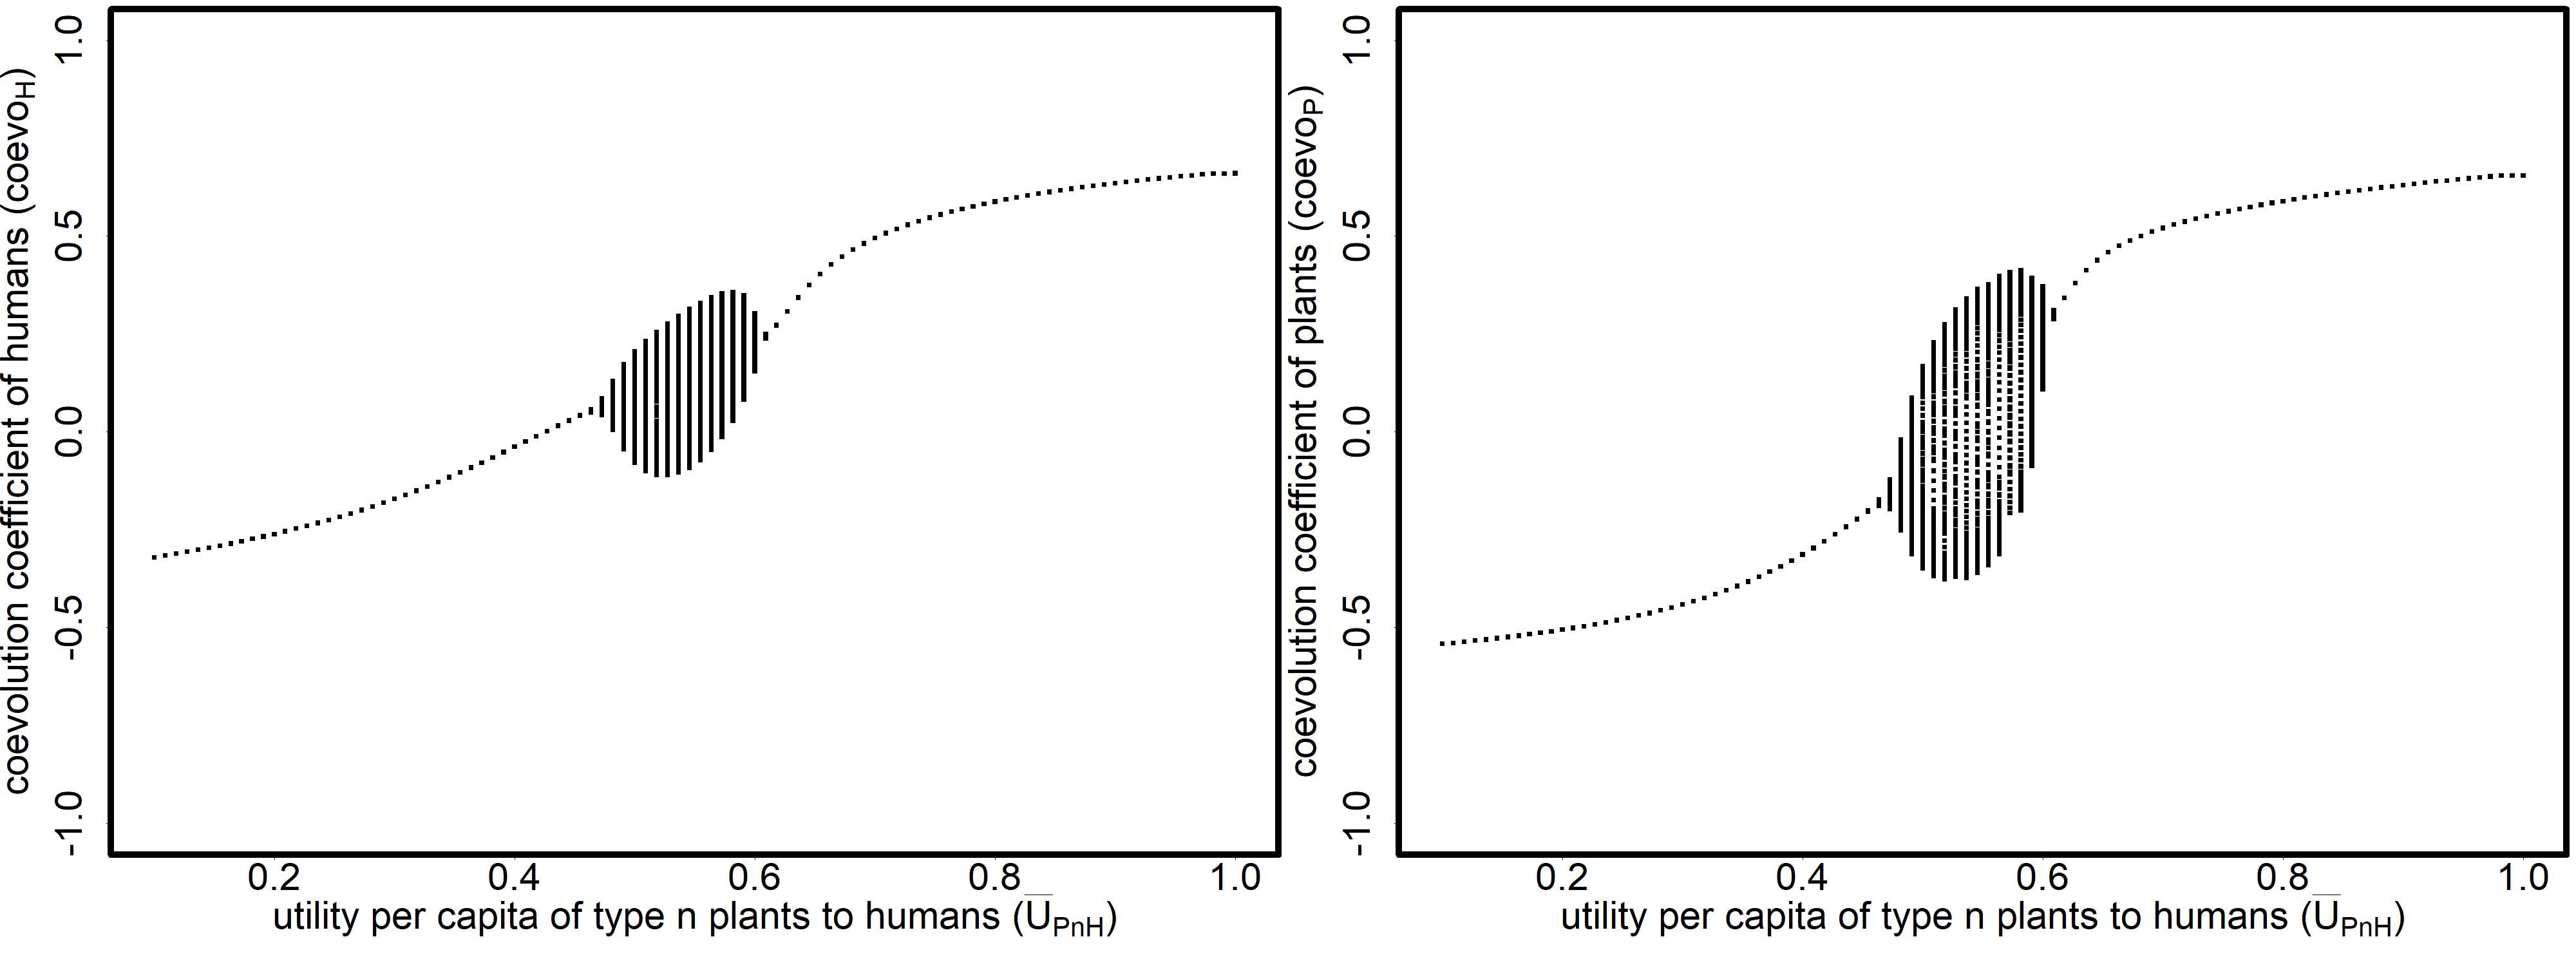
\includegraphics[width=1\linewidth]{plots/2_exp_utility_per_capita_type_n_plants_to_humans_oscillation_bifurcationPlotPair}

\hypertarget{two-parameter-exploration}{%
\chapter{Two parameter exploration}\label{two-parameter-exploration}}

\newpage

\hypertarget{full-example}{%
\section{Full example}\label{full-example}}

\hypertarget{utility-per-capita-from-type-n-humans-and-plants-baru_h_np-x-baru_p_nh}{%
\subsection{\texorpdfstring{Utility per capita from type n humans and plants (\(\bar{U}_{H_{n}P}\) x \(\bar{U}_{P_{n}H}\))}{Utility per capita from type n humans and plants (\textbackslash bar\{U\}\_\{H\_\{n\}P\} x \textbackslash bar\{U\}\_\{P\_\{n\}H\})}}\label{utility-per-capita-from-type-n-humans-and-plants-baru_h_np-x-baru_p_nh}}

\sectionmark{$\bar{U}_{H_{n}P}$ x $\bar{U}_{P_{n}H}$}

\begin{verbatim}
## [1] 31
## [1] 31
\end{verbatim}

\begin{table}[!h]

\caption{\label{tab:3mUHnPmUPnHtablepdf}Parameter setting}
\centering
\begin{tabular}[t]{l|l}
\hline
parameter & value\\
\hline
initial\_population\_humans & 10\\
\hline
initial\_population\_plants & 10\\
\hline
number\_types\_humans & 30\\
\hline
number\_types\_plants & 30\\
\hline
undirected\_variation\_humans & 0.15\\
\hline
undirected\_variation\_plants & 0.15\\
\hline
intrinsic\_growth\_rate\_humans & 0.04\\
\hline
intrinsic\_growth\_rate\_plants & 0.1\\
\hline
utility\_per\_capita\_type\_n\_plants\_to\_humans & 0 - 3 (sample = 15 )\\
\hline
utility\_per\_capita\_type\_n\_humans\_to\_plants & 0 - 3 (sample = 15 )\\
\hline
utility\_per\_capita\_type\_1\_plants\_to\_humans & 0.15\\
\hline
utility\_per\_capita\_type\_1\_humans\_to\_plants & 0\\
\hline
utility\_other\_to\_type\_n\_humans & 10\\
\hline
utility\_other\_to\_type\_n\_plants & 20\\
\hline
utility\_other\_to\_type\_1\_humans & 80\\
\hline
utility\_other\_to\_type\_1\_plants & 100\\
\hline
max\_area & 200\\
\hline
max\_iterations & 5000\\
\hline
reltol\_exponential & 6\\
\hline
coevolution\_threshold & 0.5\\
\hline
humans & 83.2614080618352 - 567.203133144437 (sample = 225 )\\
\hline
plants & 93.7854570454264 - 200 (sample = 91 )\\
\hline
coevolution\_coefficient\_humans & -0.659187038874794 - 0.700598035631623 (sample = 225 )\\
\hline
coevolution\_coefficient\_plants & -0.717940961816382 - 0.70401267833436 (sample = 215 )\\
\hline
dependency\_coefficient\_humans & -0.695128994570018 - 0.943047405719581 (sample = 225 )\\
\hline
dependency\_coefficient\_plants & -1 - 0.965964431960564 (sample = 212 )\\
\hline
timing\_humans & 0 - 797 (sample = 82 )\\
\hline
timing\_plants & 0 - 882 (sample = 83 )\\
\hline
time\_end & 380 - 1407 (sample = 122 )\\
\hline
adaptativeCost.H & 0\\
\hline
adaptativeCost.P & 0\\
\hline
\end{tabular}
\end{table}

\newpage

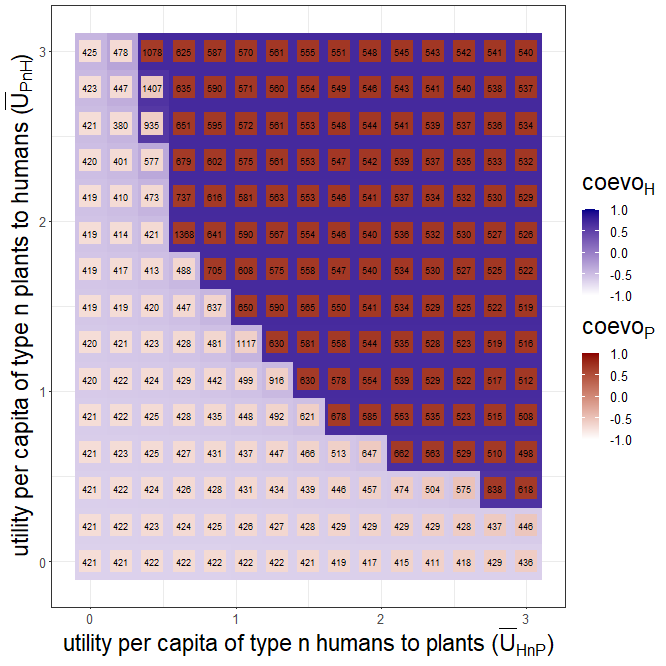
\includegraphics[width=1\linewidth]{plots/3_exp_utility_per_capita_type_n-tripleRaster_twoParameters}

\newpage

\hypertarget{exploration-on-default-setting-for-parameter-pairs}{%
\section{Exploration on `default' setting for parameter pairs}\label{exploration-on-default-setting-for-parameter-pairs}}

\hypertarget{number-of-types-of-humans-and-plants-n_h-x-n_p}{%
\subsection{\texorpdfstring{Number of types of humans and plants (\(n_{H}\) x \(n_{P}\))}{Number of types of humans and plants (n\_\{H\} x n\_\{P\})}}\label{number-of-types-of-humans-and-plants-n_h-x-n_p}}

\sectionmark{$n_{H}$ x $n_{P}$}

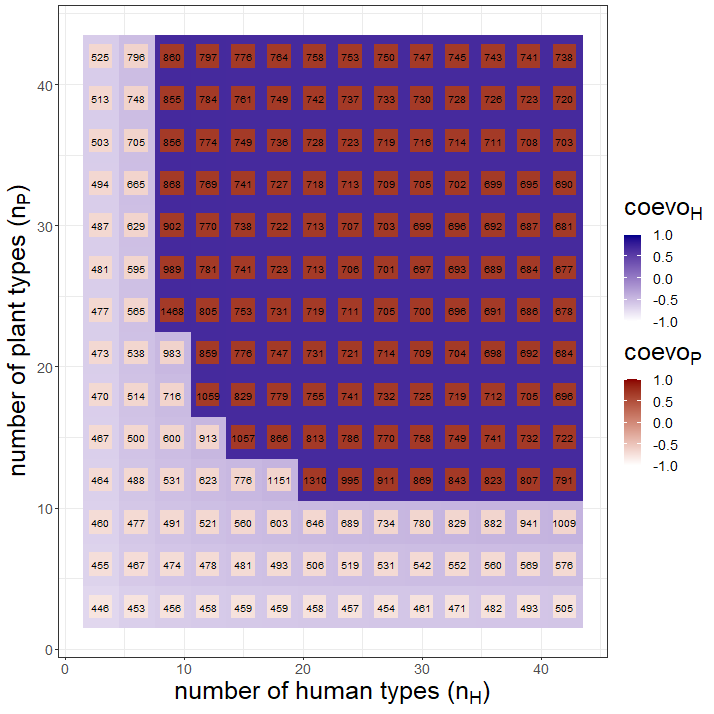
\includegraphics[width=1\linewidth]{plots/3_exp_number_types-tripleRaster_twoParameters}

\newpage

\hypertarget{undirected-variation-in-humans-and-plants-v_h-x-v_p}{%
\subsection{\texorpdfstring{Undirected variation in humans and plants (\(v_{H}\) x \(v_{P}\))}{Undirected variation in humans and plants (v\_\{H\} x v\_\{P\})}}\label{undirected-variation-in-humans-and-plants-v_h-x-v_p}}

\sectionmark{$v_{H}$ x $v_{P}$}

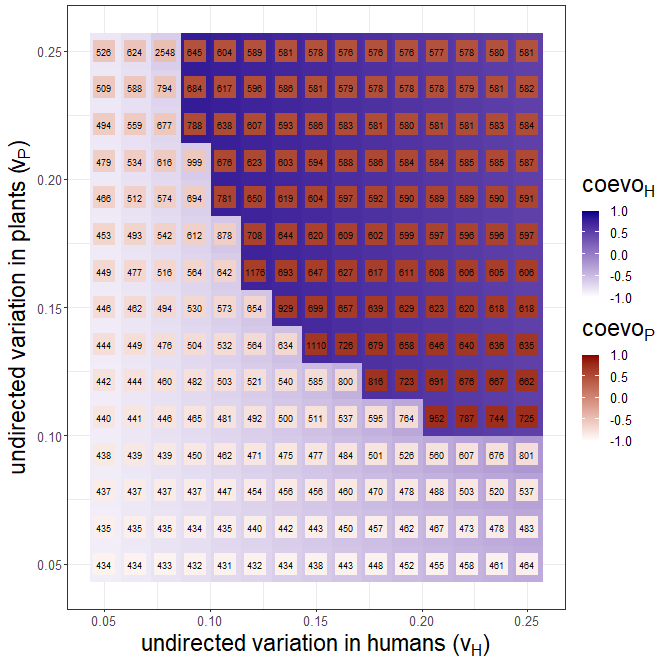
\includegraphics[width=1\linewidth]{plots/3_exp_undirected_variation-tripleRaster_twoParameters}

\newpage

\hypertarget{utility-per-capita-from-type-1-humans-and-plants-baru_h_1p-x-baru_p_1h}{%
\subsection{\texorpdfstring{Utility per capita from type 1 humans and plants (\(\bar{U}_{H_{1}P}\) x \(\bar{U}_{P_{1}H}\))}{Utility per capita from type 1 humans and plants (\textbackslash bar\{U\}\_\{H\_\{1\}P\} x \textbackslash bar\{U\}\_\{P\_\{1\}H\})}}\label{utility-per-capita-from-type-1-humans-and-plants-baru_h_1p-x-baru_p_1h}}

\sectionmark{$\bar{U}_{H_{1}P}$ x $\bar{U}_{P_{1}H}$}

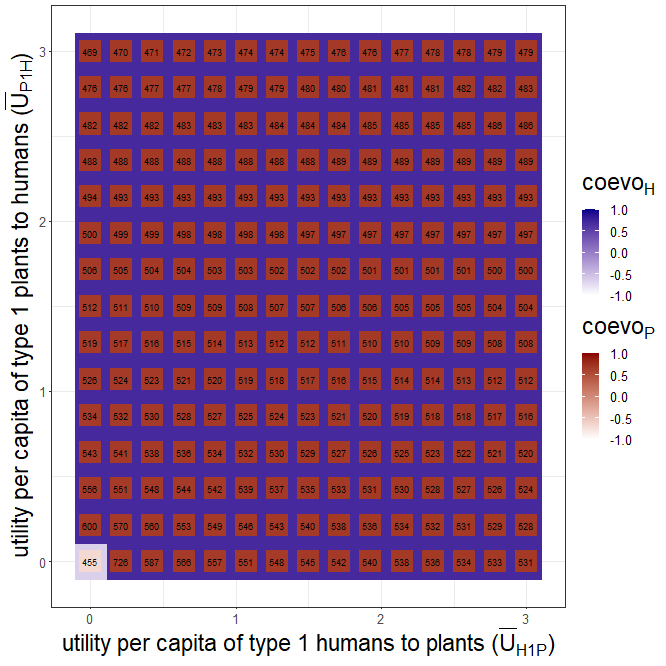
\includegraphics[width=1\linewidth]{plots/3_exp_utility_per_capita_type_1-tripleRaster_twoParameters}

\newpage

\hypertarget{utility-per-capita-from-type-n-humans-and-plants-baru_h_np-x-baru_p_nh-1}{%
\subsection{\texorpdfstring{Utility per capita from type n humans and plants (\(\bar{U}_{H_{n}P}\) x \(\bar{U}_{P_{n}H}\))}{Utility per capita from type n humans and plants (\textbackslash bar\{U\}\_\{H\_\{n\}P\} x \textbackslash bar\{U\}\_\{P\_\{n\}H\})}}\label{utility-per-capita-from-type-n-humans-and-plants-baru_h_np-x-baru_p_nh-1}}

\sectionmark{$\bar{U}_{H_{n}P}$ x $\bar{U}_{P_{n}H}$}

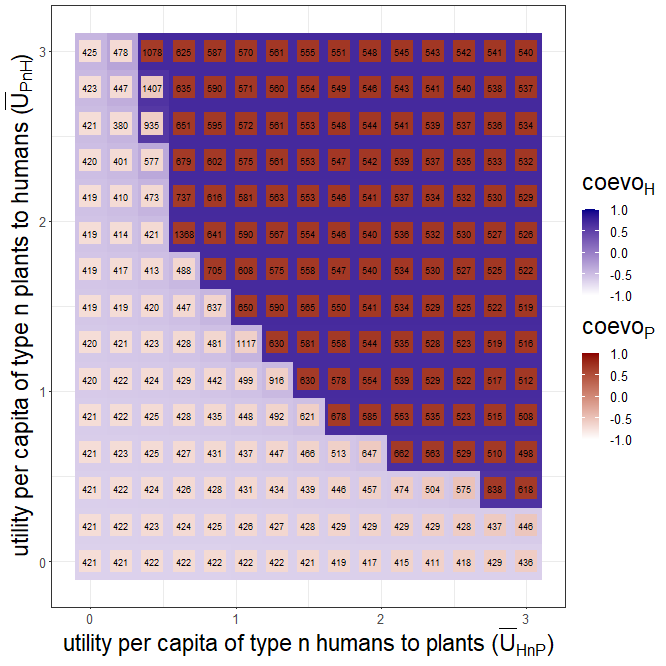
\includegraphics[width=1\linewidth]{plots/3_exp_utility_per_capita_type_n-tripleRaster_twoParameters}

\newpage

\hypertarget{utility-per-capita-from-humans-to-plants-baru_h_1p-x-baru_h_np}{%
\subsection{\texorpdfstring{Utility per capita from humans to plants (\(\bar{U}_{H_{1}P}\) x \(\bar{U}_{H_{n}P}\))}{Utility per capita from humans to plants (\textbackslash bar\{U\}\_\{H\_\{1\}P\} x \textbackslash bar\{U\}\_\{H\_\{n\}P\})}}\label{utility-per-capita-from-humans-to-plants-baru_h_1p-x-baru_h_np}}

\sectionmark{$\bar{U}_{H_{1}P}$ x $\bar{U}_{H_{n}P}$}

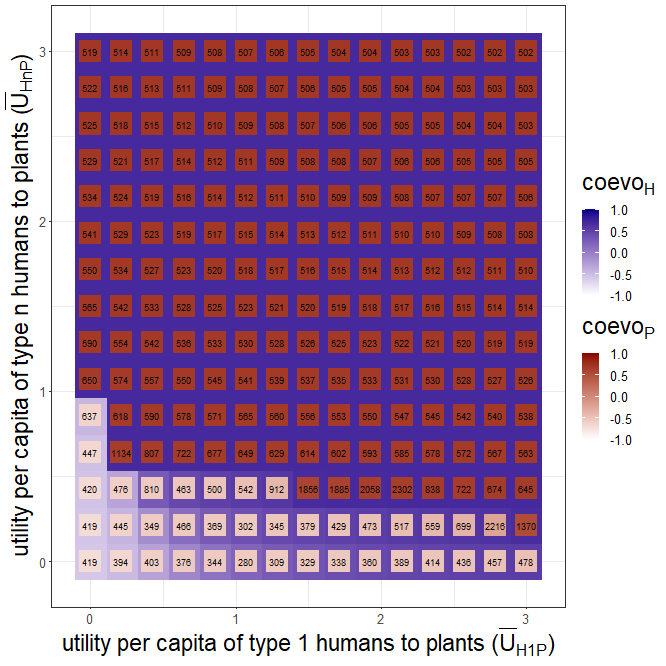
\includegraphics[width=1\linewidth]{plots/3_exp_utility_per_capita_type_humans_to_plants-tripleRaster_twoParameters}

\newpage

\hypertarget{utility-per-capita-from-plants-to-humans-baru_p_1h-x-baru_p_nh}{%
\subsection{\texorpdfstring{Utility per capita from plants to humans (\(\bar{U}_{P_{1}H}\) x \(\bar{U}_{P_{n}H}\))}{Utility per capita from plants to humans (\textbackslash bar\{U\}\_\{P\_\{1\}H\} x \textbackslash bar\{U\}\_\{P\_\{n\}H\})}}\label{utility-per-capita-from-plants-to-humans-baru_p_1h-x-baru_p_nh}}

\sectionmark{$\bar{U}_{P_{1}H}$ x $\bar{U}_{P_{n}H}$}

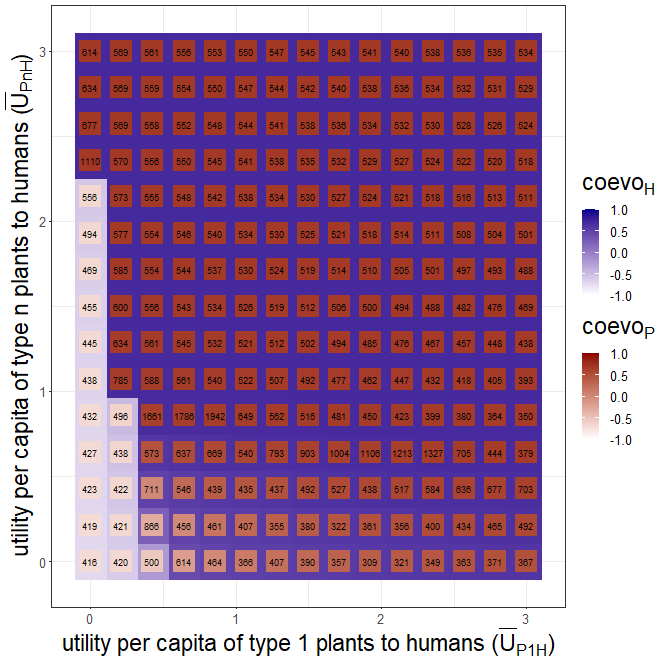
\includegraphics[width=1\linewidth]{plots/3_exp_utility_per_capita_type_plants_to_humans-tripleRaster_twoParameters}

\newpage

\hypertarget{utility-of-other-resources-to-type-1-humans-and-plants-u_bh_1-x-u_bp_1}{%
\subsection{\texorpdfstring{Utility of other resources to type 1 humans and plants (\(U_{bH_{1}}\) x \(U_{bP_{1}}\))}{Utility of other resources to type 1 humans and plants (U\_\{bH\_\{1\}\} x U\_\{bP\_\{1\}\})}}\label{utility-of-other-resources-to-type-1-humans-and-plants-u_bh_1-x-u_bp_1}}

\sectionmark{$U_{bH_{1}}$ x $U_{bP_{1}}$}

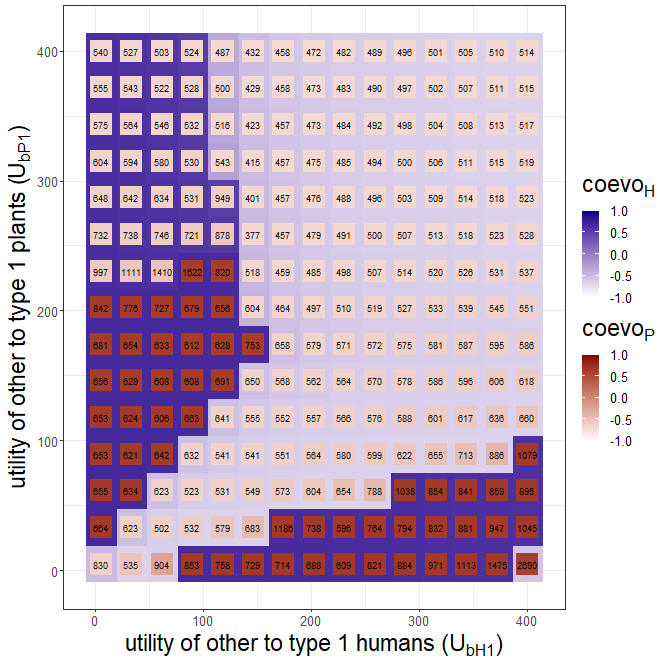
\includegraphics[width=1\linewidth]{plots/3_exp_utility_other_to_type_1-tripleRaster_twoParameters}

\newpage

\hypertarget{utility-of-other-resources-to-type-n-humans-and-plants-u_bh_n-x-u_bp_n}{%
\subsection{\texorpdfstring{Utility of other resources to type n humans and plants (\(U_{bH_{n}}\) x \(U_{bP_{n}}\))}{Utility of other resources to type n humans and plants (U\_\{bH\_\{n\}\} x U\_\{bP\_\{n\}\})}}\label{utility-of-other-resources-to-type-n-humans-and-plants-u_bh_n-x-u_bp_n}}

\sectionmark{$U_{bH_{n}}$ x $U_{bP_{n}}$}

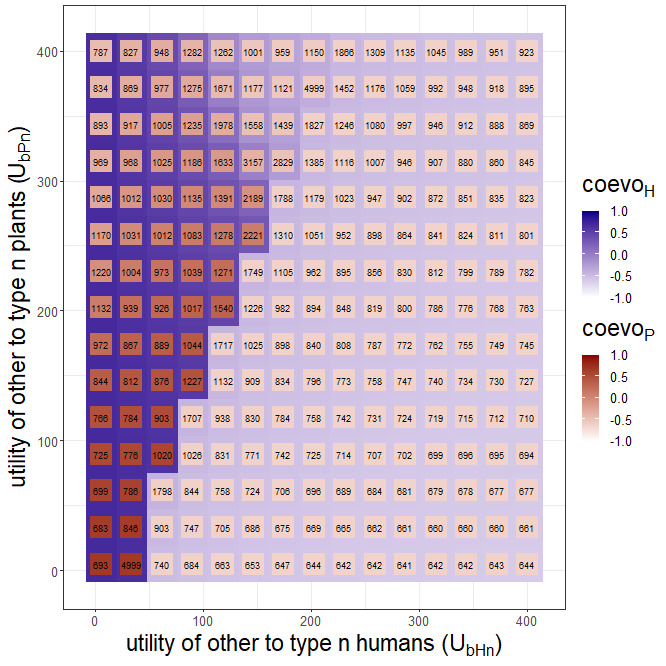
\includegraphics[width=1\linewidth]{plots/3_exp_utility_other_to_type_n-tripleRaster_twoParameters}

\newpage

\hypertarget{utility-of-other-resources-to-humans-u_bh_1-x-u_bh_n}{%
\subsection{\texorpdfstring{Utility of other resources to humans (\(U_{bH_{1}}\) x \(U_{bH_{n}}\))}{Utility of other resources to humans (U\_\{bH\_\{1\}\} x U\_\{bH\_\{n\}\})}}\label{utility-of-other-resources-to-humans-u_bh_1-x-u_bh_n}}

\sectionmark{$U_{bH_{1}}$ x $U_{bH_{n}}$}

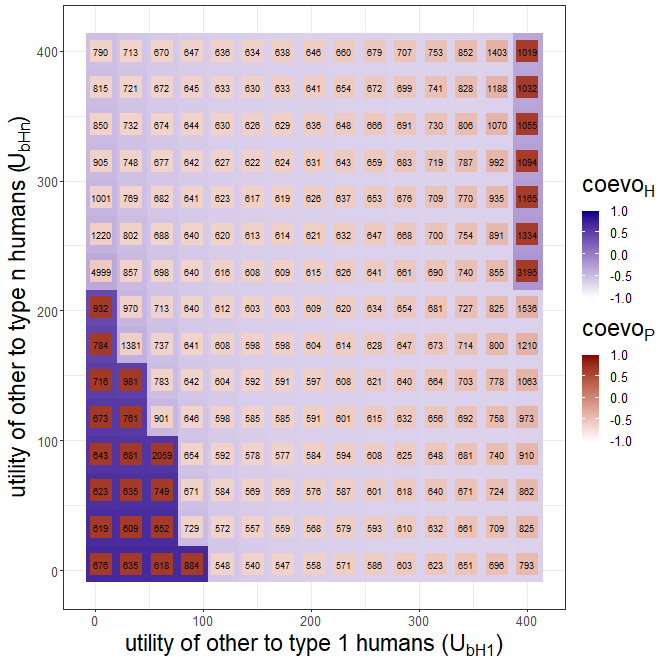
\includegraphics[width=1\linewidth]{plots/3_exp_utility_other_to_type_humans-tripleRaster_twoParameters}

\newpage

\hypertarget{utility-of-other-resources-to-plants-u_bp_1-x-u_bp_n}{%
\subsection{\texorpdfstring{Utility of other resources to plants (\(U_{bP_{1}}\) x \(U_{bP_{n}}\))}{Utility of other resources to plants (U\_\{bP\_\{1\}\} x U\_\{bP\_\{n\}\})}}\label{utility-of-other-resources-to-plants-u_bp_1-x-u_bp_n}}

\sectionmark{$U_{bP_{1}}$ x $U_{bP_{n}}$}

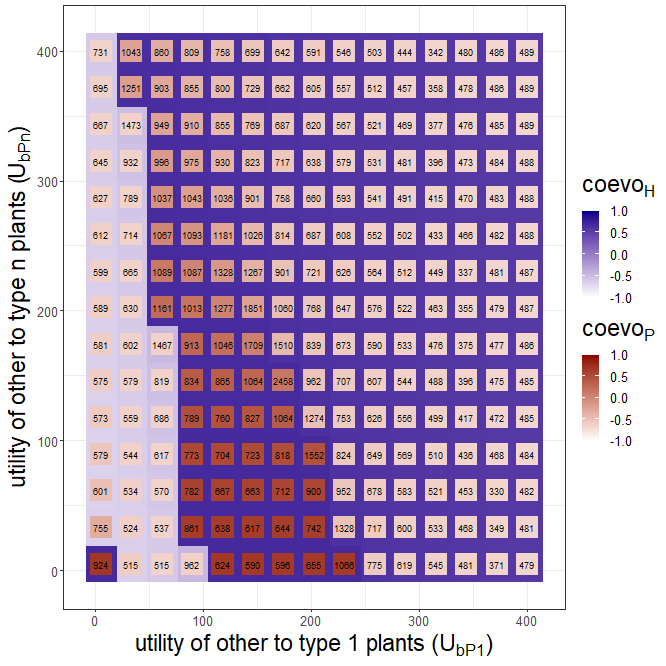
\includegraphics[width=1\linewidth]{plots/3_exp_utility_other_to_type_plants-tripleRaster_twoParameters}

\hypertarget{utility-of-other-resources-to-type-1-humans-and-utility-per-capita-of-type-1-humans-to-plants-u_bh_1-x-baru_h_1p}{%
\subsection{\texorpdfstring{Utility of other resources to type 1 humans and utility per capita of type 1 humans to plants (\(U_{bH_{1}}\) x \(\bar{U}_{H_{1}P}\))}{Utility of other resources to type 1 humans and utility per capita of type 1 humans to plants (U\_\{bH\_\{1\}\} x \textbackslash bar\{U\}\_\{H\_\{1\}P\})}}\label{utility-of-other-resources-to-type-1-humans-and-utility-per-capita-of-type-1-humans-to-plants-u_bh_1-x-baru_h_1p}}

\sectionmark{$U_{bH_{1}}$ x $\bar{U}_{H_{1}P}$}

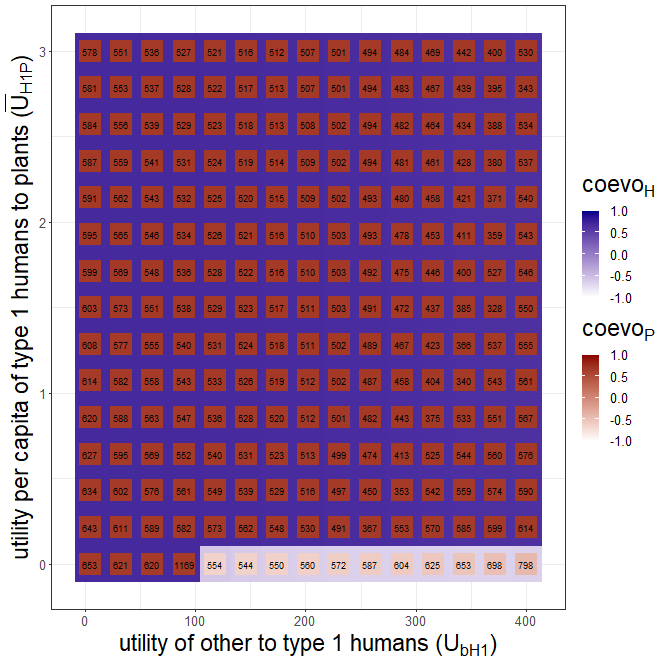
\includegraphics[width=1\linewidth]{plots/3_exp_type_1_humans_traits-tripleRaster_twoParameters}

\newpage

\hypertarget{utility-of-other-resources-to-type-1-plants-and-utility-per-capita-of-type-1-plants-to-humans-u_bp_1-x-baru_p_1h}{%
\subsection{\texorpdfstring{Utility of other resources to type 1 plants and utility per capita of type 1 plants to humans (\(U_{bP_{1}}\) x \(\bar{U}_{P_{1}H}\))}{Utility of other resources to type 1 plants and utility per capita of type 1 plants to humans (U\_\{bP\_\{1\}\} x \textbackslash bar\{U\}\_\{P\_\{1\}H\})}}\label{utility-of-other-resources-to-type-1-plants-and-utility-per-capita-of-type-1-plants-to-humans-u_bp_1-x-baru_p_1h}}

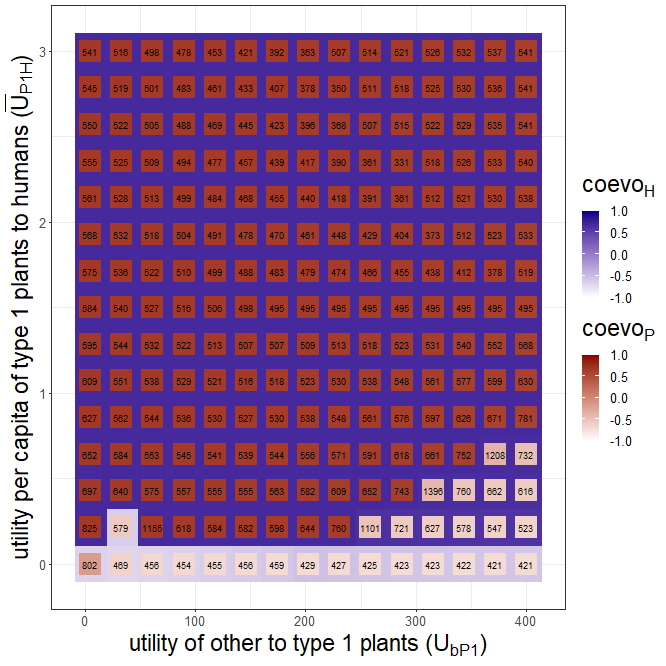
\includegraphics[width=1\linewidth]{plots/3_exp_type_1_plants_traits-tripleRaster_twoParameters}

\newpage

\hypertarget{utility-of-other-resources-to-type-n-humans-and-utility-per-capita-of-type-n-humans-to-plants-u_bh_n-x-baru_h_np}{%
\subsection{\texorpdfstring{Utility of other resources to type n humans and utility per capita of type n humans to plants (\(U_{bH_{n}}\) x \(\bar{U}_{H_{n}P}\))}{Utility of other resources to type n humans and utility per capita of type n humans to plants (U\_\{bH\_\{n\}\} x \textbackslash bar\{U\}\_\{H\_\{n\}P\})}}\label{utility-of-other-resources-to-type-n-humans-and-utility-per-capita-of-type-n-humans-to-plants-u_bh_n-x-baru_h_np}}

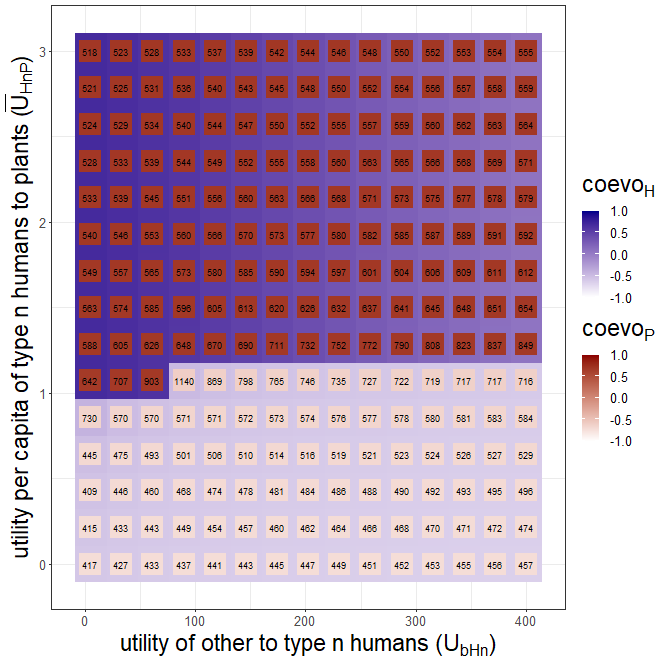
\includegraphics[width=1\linewidth]{plots/3_exp_type_n_humans_traits-tripleRaster_twoParameters}

\newpage

\hypertarget{utility-of-other-resources-to-type-n-plants-and-utility-per-capita-of-type-n-plants-to-humans-u_bp_n-x-baru_p_nh}{%
\subsection{\texorpdfstring{Utility of other resources to type n plants and utility per capita of type n plants to humans (\(U_{bP_{n}}\) x \(\bar{U}_{P_{n}H}\))}{Utility of other resources to type n plants and utility per capita of type n plants to humans (U\_\{bP\_\{n\}\} x \textbackslash bar\{U\}\_\{P\_\{n\}H\})}}\label{utility-of-other-resources-to-type-n-plants-and-utility-per-capita-of-type-n-plants-to-humans-u_bp_n-x-baru_p_nh}}

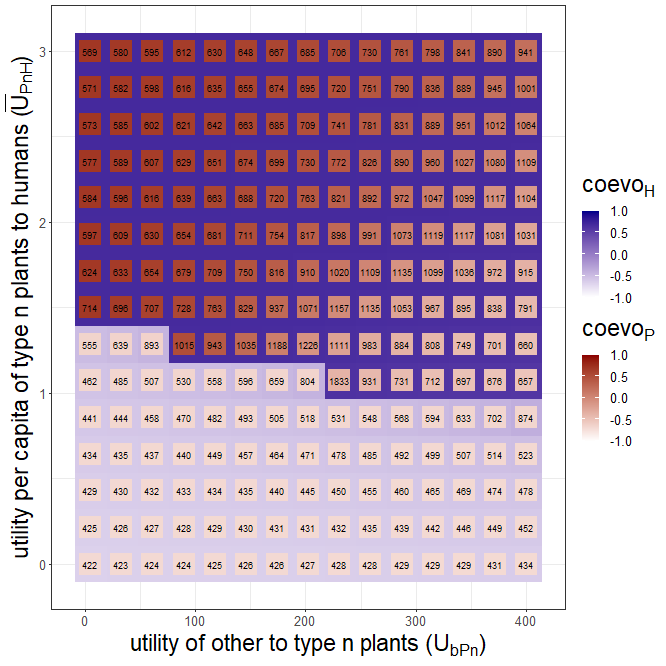
\includegraphics[width=1\linewidth]{plots/3_exp_type_n_plants_traits-tripleRaster_twoParameters}

\newpage

\hypertarget{four-parameter-exploration}{%
\chapter{Four parameter exploration}\label{four-parameter-exploration}}

\newpage

\hypertarget{number-of-types-and-undirected-variation-of-humans-and-plants-n_h-x-n_p-x-v_h-x-v_p}{%
\section{\texorpdfstring{Number of types and undirected variation of humans and plants (\(n_{H}\) x \(n_{P}\) x \(v_{H}\) x \(v_{P}\))}{Number of types and undirected variation of humans and plants (n\_\{H\} x n\_\{P\} x v\_\{H\} x v\_\{P\})}}\label{number-of-types-and-undirected-variation-of-humans-and-plants-n_h-x-n_p-x-v_h-x-v_p}}

\sectionmark{$n_{H}$ x $n_{P}$ x $v_{H}$ x $v_{P}$}

\begin{table}[!h]

\caption{\label{tab:4nvtablepdf}Parameter setting}
\centering
\begin{tabular}[t]{l|l}
\hline
parameter & value\\
\hline
initial\_population\_humans & 10\\
\hline
initial\_population\_plants & 10\\
\hline
number\_types\_humans & 5 - 45 (sample = 5 )\\
\hline
number\_types\_plants & 5 - 45 (sample = 5 )\\
\hline
undirected\_variation\_humans & 0.05 - 0.25 (sample = 5 )\\
\hline
undirected\_variation\_plants & 0.05 - 0.25 (sample = 5 )\\
\hline
intrinsic\_growth\_rate\_humans & 0.04\\
\hline
intrinsic\_growth\_rate\_plants & 0.1\\
\hline
utility\_per\_capita\_type\_n\_plants\_to\_humans & 1.5\\
\hline
utility\_per\_capita\_type\_n\_humans\_to\_plants & 1\\
\hline
utility\_per\_capita\_type\_1\_plants\_to\_humans & 0.15\\
\hline
utility\_per\_capita\_type\_1\_humans\_to\_plants & 0\\
\hline
utility\_other\_to\_type\_n\_humans & 10\\
\hline
utility\_other\_to\_type\_n\_plants & 20\\
\hline
utility\_other\_to\_type\_1\_humans & 80\\
\hline
utility\_other\_to\_type\_1\_plants & 100\\
\hline
max\_area & 200\\
\hline
max\_iterations & 5000\\
\hline
reltol\_exponential & 6\\
\hline
coevolution\_threshold & 0.5\\
\hline
humans & 85.1414283817248 - 303.920561546526 (sample = 625 )\\
\hline
plants & 93.5982997036815 - 200 (sample = 372 )\\
\hline
coevolution\_coefficient\_humans & -0.893138319410505 - 0.796970470817761 (sample = 625 )\\
\hline
coevolution\_coefficient\_plants & -0.918044258212089 - 0.784003454561172 (sample = 625 )\\
\hline
dependency\_coefficient\_humans & -0.632605349151667 - 0.897316999088837 (sample = 625 )\\
\hline
dependency\_coefficient\_plants & -0.943727131580906 - 0.820755925015822 (sample = 625 )\\
\hline
timing\_humans & 0 - 1117 (sample = 131 )\\
\hline
timing\_plants & 0 - 1074 (sample = 84 )\\
\hline
time\_end & 427 - 3284 (sample = 240 )\\
\hline
adaptativeCost.H & 0\\
\hline
adaptativeCost.P & 0\\
\hline
\end{tabular}
\end{table}

\newpage

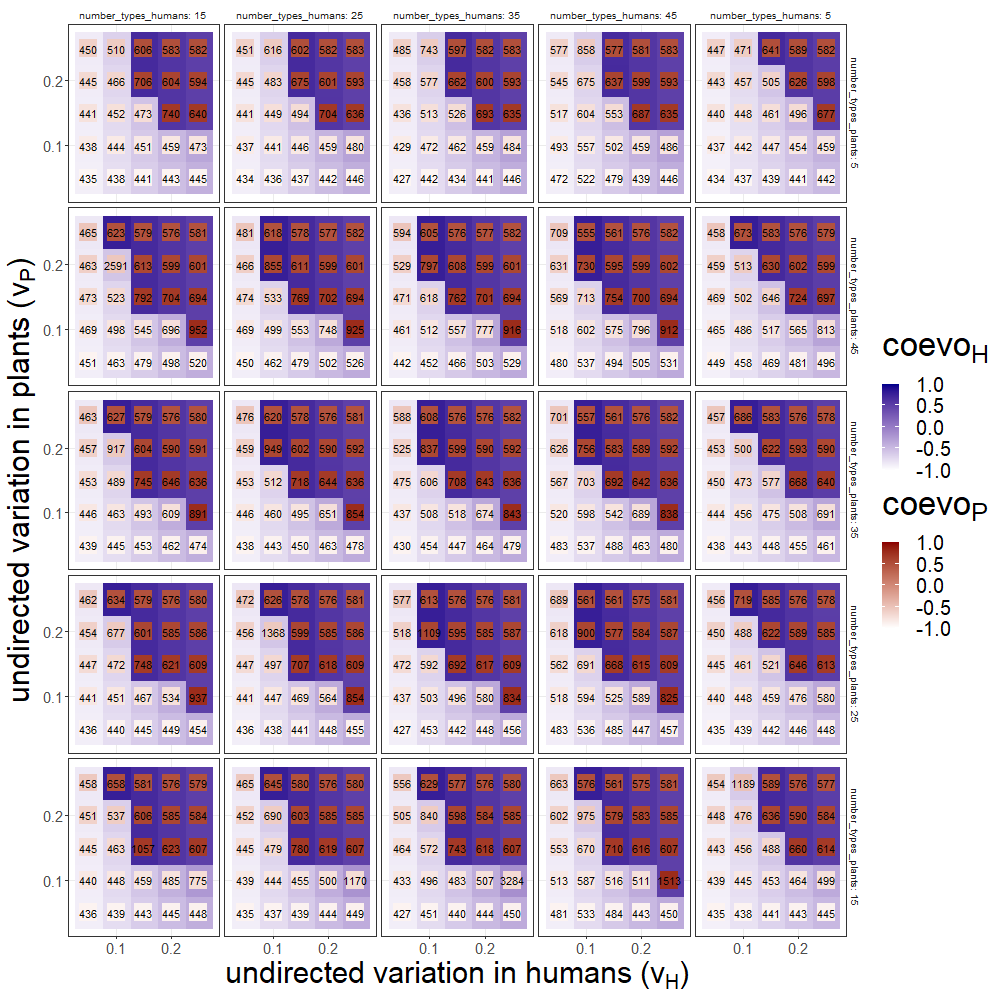
\includegraphics[width=1\linewidth]{plots/4_exp_types_number_and_variation-tripleRaster_fourParameterss}

\textbf{\emph{Interpretation}}:\\
- Higher values of all four parameters facilitate coevolution. Undirected variation has a stronger effect than number of types.
- As a summary of possible end-states:\\
+ \emph{`Fast' coevolution} (red square in blue tile, small \emph{t}): most cases when the numbers of types (\(n_{H}\), \(n_{P}\)) are greater than \textbf{15} and values of undirected variation (\(v_{H}\), \(v_{P}\)) higher than \textbf{0.15}.\\
+ \emph{`Semi-domestication' without cultivation} (redish square in whitish tile): cases when \(v_{P}\geq 0.15\) and \(v_{H}\leq 0.15\).\\
+ \emph{`Semi-cultivation' without domestication} (whitish square in blue tile): cases when \(v_{H}\geq 0.15\) and \(v_{P}\leq 0.15\).

\newpage

\hypertarget{utility-per-capita-between-humans-and-plants-baru_h_1p-x-baru_p_1h-x-baru_h_np-x-baru_p_nh}{%
\section{\texorpdfstring{Utility per capita between humans and plants (\(\bar{U}_{H_{1}P}\) x \(\bar{U}_{P_{1}H}\) x \(\bar{U}_{H_{n}P}\) x \(\bar{U}_{P_{n}H}\))}{Utility per capita between humans and plants (\textbackslash bar\{U\}\_\{H\_\{1\}P\} x \textbackslash bar\{U\}\_\{P\_\{1\}H\} x \textbackslash bar\{U\}\_\{H\_\{n\}P\} x \textbackslash bar\{U\}\_\{P\_\{n\}H\})}}\label{utility-per-capita-between-humans-and-plants-baru_h_1p-x-baru_p_1h-x-baru_h_np-x-baru_p_nh}}

\sectionmark{$\bar{U}_{H_{1}P}$ x $\bar{U}_{P_{1}H}$ x $\bar{U}_{H_{n}P}$ x $\bar{U}_{P_{n}H}$}

\begin{table}[!h]

\caption{\label{tab:4mUHPmUPHtablepdf}Parameter setting}
\centering
\begin{tabular}[t]{l|l}
\hline
parameter & value\\
\hline
initial\_population\_humans & 10\\
\hline
initial\_population\_plants & 10\\
\hline
number\_types\_humans & 30\\
\hline
number\_types\_plants & 30\\
\hline
undirected\_variation\_humans & 0.15\\
\hline
undirected\_variation\_plants & 0.15\\
\hline
intrinsic\_growth\_rate\_humans & 0.04\\
\hline
intrinsic\_growth\_rate\_plants & 0.1\\
\hline
utility\_per\_capita\_type\_n\_plants\_to\_humans & 0 - 3 (sample = 5 )\\
\hline
utility\_per\_capita\_type\_n\_humans\_to\_plants & 0 - 3 (sample = 5 )\\
\hline
utility\_per\_capita\_type\_1\_plants\_to\_humans & 0 - 3 (sample = 5 )\\
\hline
utility\_per\_capita\_type\_1\_humans\_to\_plants & 0 - 3 (sample = 5 )\\
\hline
utility\_other\_to\_type\_n\_humans & 10\\
\hline
utility\_other\_to\_type\_n\_plants & 20\\
\hline
utility\_other\_to\_type\_1\_humans & 80\\
\hline
utility\_other\_to\_type\_1\_plants & 100\\
\hline
max\_area & 200\\
\hline
max\_iterations & 5000\\
\hline
reltol\_exponential & 6\\
\hline
coevolution\_threshold & 0.5\\
\hline
humans & 74.5622526385153 - 616.122991274673 (sample = 611 )\\
\hline
plants & 93.7854569646093 - 200 (sample = 222 )\\
\hline
coevolution\_coefficient\_humans & -0.717940961994967 - 0.701298246126613 (sample = 611 )\\
\hline
coevolution\_coefficient\_plants & -0.717941007482056 - 0.704797600572959 (sample = 625 )\\
\hline
dependency\_coefficient\_humans & -1 - 0.947663005457465 (sample = 601 )\\
\hline
dependency\_coefficient\_plants & -1 - 0.971381159245891 (sample = 602 )\\
\hline
timing\_humans & 0 - 219 (sample = 70 )\\
\hline
timing\_plants & 0 - 290 (sample = 85 )\\
\hline
time\_end & 300 - 4999 (sample = 248 )\\
\hline
adaptativeCost.H & 0\\
\hline
adaptativeCost.P & 0\\
\hline
\end{tabular}
\end{table}

\newpage

\includegraphics[width=1\linewidth]{plots/4_exp_utilities_between_populations-tripleRaster_fourParameterss}

\textbf{\emph{Interpretation}}:\\
- Higher values of all four parameters facilitate coevolution; under the `default' setting, a value around 1 is enough for all four parameters (intermediate values in this exploration).\\
- Coevolution is still possible if any single one of these parameters equal zero (first rows or first columns). Under this type of conditions, cultivation (blue) is more probable than domestication (red), and the latter is strongly dependent on a non-null \(\bar{U}_{H_{n}P}\).\\
- As a summary of possible end-states:\\
+ \emph{`Fast' coevolution} (red square in blue tile, small \emph{t}): most cases when values are greater than 0.75.\\
+ \emph{Domestication without cultivation} (red square in whitish tile): most cases when \(\bar{U}_{H_{n}P}>0.75\), \(\bar{U}_{H_{1}P}\geq 0.75\), \(\bar{U}_{P_{n}H}=0\), and \(\bar{U}_{P_{1}H}<2\).\\
+ \emph{Cultivation without domestication} (whitish square in blue tile): most cases when \(\bar{U}_{H_{n}P} = 0\).

\newpage

\hypertarget{utility-from-other-resources-to-humans-and-plants-u_bh_1-x-u_bp_1-x-u_bh_n-x-u_bp_n}{%
\section{\texorpdfstring{Utility from other resources to humans and plants (\(U_{bH_{1}}\) x \(U_{bP_{1}}\) x \(U_{bH_{n}}\) x \(U_{bP_{n}}\))}{Utility from other resources to humans and plants (U\_\{bH\_\{1\}\} x U\_\{bP\_\{1\}\} x U\_\{bH\_\{n\}\} x U\_\{bP\_\{n\}\})}}\label{utility-from-other-resources-to-humans-and-plants-u_bh_1-x-u_bp_1-x-u_bh_n-x-u_bp_n}}

\sectionmark{$U_{bH_{1}}$ x $U_{bP_{1}}$ x $U_{bH_{n}}$ x $U_{bP_{n}}$}

For this experiment, consider that the default setting includes \(MaxArea=200\) (i.e.~the maximum for the plant population).

\begin{table}[!h]

\caption{\label{tab:4UbHUbPtablepdf}Parameter setting}
\centering
\begin{tabular}[t]{l|l}
\hline
parameter & value\\
\hline
initial\_population\_humans & 10\\
\hline
initial\_population\_plants & 10\\
\hline
number\_types\_humans & 30\\
\hline
number\_types\_plants & 30\\
\hline
undirected\_variation\_humans & 0.15\\
\hline
undirected\_variation\_plants & 0.15\\
\hline
intrinsic\_growth\_rate\_humans & 0.04\\
\hline
intrinsic\_growth\_rate\_plants & 0.1\\
\hline
utility\_per\_capita\_type\_n\_plants\_to\_humans & 1.5\\
\hline
utility\_per\_capita\_type\_n\_humans\_to\_plants & 1\\
\hline
utility\_per\_capita\_type\_1\_plants\_to\_humans & 0.15\\
\hline
utility\_per\_capita\_type\_1\_humans\_to\_plants & 0\\
\hline
utility\_other\_to\_type\_n\_humans & 5 - 300 (sample = 5 )\\
\hline
utility\_other\_to\_type\_n\_plants & 5 - 300 (sample = 5 )\\
\hline
utility\_other\_to\_type\_1\_humans & 5 - 300 (sample = 5 )\\
\hline
utility\_other\_to\_type\_1\_plants & 5 - 300 (sample = 5 )\\
\hline
max\_area & 200\\
\hline
max\_iterations & 5000\\
\hline
reltol\_exponential & 6\\
\hline
coevolution\_threshold & 0.5\\
\hline
humans & 7.02756257875232 - 560.973786604167 (sample = 625 )\\
\hline
plants & 6.24776319282656 - 200 (sample = 256 )\\
\hline
coevolution\_coefficient\_humans & -0.662899373475303 - 0.703777349450851 (sample = 625 )\\
\hline
coevolution\_coefficient\_plants & -0.682616984408088 - 0.704560157675581 (sample = 625 )\\
\hline
dependency\_coefficient\_humans & -0.709161863456466 - 0.964351497555221 (sample = 625 )\\
\hline
dependency\_coefficient\_plants & -0.793157825095748 - 0.969736541196175 (sample = 625 )\\
\hline
timing\_humans & 0 - 1593 (sample = 54 )\\
\hline
timing\_plants & 0 - 2475 (sample = 54 )\\
\hline
time\_end & 359 - 4999 (sample = 362 )\\
\hline
adaptativeCost.H & 0\\
\hline
adaptativeCost.P & 0\\
\hline
\end{tabular}
\end{table}

\newpage

\includegraphics[width=1\linewidth]{plots/4_exp_utilities_other_to_populations-tripleRaster_fourParameterss}

\textbf{\emph{Interpretation}}:\\
- Lower values of the two human-related parameters (\(U_{bH_{1}}\), \(U_{bH_{n}}\)) facilitate coevolution; under the `default' setting and for all four parameters, values greater or equal to \(MaxArea\) (here, 200) impede coevolution. Inversely, higher values of the plant-related parameters (\(U_{bP_{1}}\), \(U_{bP_{n}}\)) facilitate coevolution. The human-related parameters, together regulating the scale of the subsistence alternatives for humans, are significantly more important; their relationship (if one is greater than the other) seems to be less important as long as their combined sum is small enough.\\
- Coevolution is likely to occur when \(U_{bH_{1}}=5\) (first row in small grids), unless \(U_{bH_{n}}\) is too big and \(U_{bP_{1}}\) is too small.\\
- As a summary of possible end-states:\\
+ \emph{`Fast' coevolution} (red square in blue tile, small \emph{t}): most cases when \(U_{bH_{1}}\) and \(U_{bH_{n}}<153\).\\
+ \emph{Domestication without cultivation} (red square in whitish tile): most cases when \(U_{bP_{n}}=5\), \(U_{bP_{1}}=5\) (i.e.~there is very little carrying capacity for plants beyond the anthropic space) and \(U_{bH_{1}}>5\) (i.e.~humans get enough of other resources when -still- not engaged in agriculture).\\
+ \emph{Cultivation without domestication} (whitish square in blue tile): \emph{no cases are visible under these conditions}.

\newpage

\hypertarget{utility-from-other-resources-to-humans-and-utility-per-capita-of-plants-to-humans-u_bh_1-x-u_bh_n-x-baru_p_1h-x-baru_p_nh}{%
\section{\texorpdfstring{Utility from other resources to humans and utility per capita of plants to humans (\(U_{bH_{1}}\) x \(U_{bH_{n}}\) x \(\bar{U}_{P_{1}H}\) x \(\bar{U}_{P_{n}H}\))}{Utility from other resources to humans and utility per capita of plants to humans (U\_\{bH\_\{1\}\} x U\_\{bH\_\{n\}\} x \textbackslash bar\{U\}\_\{P\_\{1\}H\} x \textbackslash bar\{U\}\_\{P\_\{n\}H\})}}\label{utility-from-other-resources-to-humans-and-utility-per-capita-of-plants-to-humans-u_bh_1-x-u_bh_n-x-baru_p_1h-x-baru_p_nh}}

\sectionmark{$U_{bH_{1}}$ x $U_{bH_{n}}$ x $\bar{U}_{P_{1}H}$ x $\bar{U}_{P_{n}H}$}

All four parameters affect directly the carrying capacity for humans.

\begin{table}[!h]

\caption{\label{tab:4UbHUPHtablepdf}Parameter setting}
\centering
\begin{tabular}[t]{l|l}
\hline
parameter & value\\
\hline
initial\_population\_humans & 10\\
\hline
initial\_population\_plants & 10\\
\hline
number\_types\_humans & 30\\
\hline
number\_types\_plants & 30\\
\hline
undirected\_variation\_humans & 0.15\\
\hline
undirected\_variation\_plants & 0.15\\
\hline
intrinsic\_growth\_rate\_humans & 0.04\\
\hline
intrinsic\_growth\_rate\_plants & 0.1\\
\hline
utility\_per\_capita\_type\_n\_plants\_to\_humans & 0 - 3 (sample = 5 )\\
\hline
utility\_per\_capita\_type\_n\_humans\_to\_plants & 1\\
\hline
utility\_per\_capita\_type\_1\_plants\_to\_humans & 0 - 3 (sample = 5 )\\
\hline
utility\_per\_capita\_type\_1\_humans\_to\_plants & 0\\
\hline
utility\_other\_to\_type\_n\_humans & 5 - 300 (sample = 5 )\\
\hline
utility\_other\_to\_type\_n\_plants & 20\\
\hline
utility\_other\_to\_type\_1\_humans & 5 - 300 (sample = 5 )\\
\hline
utility\_other\_to\_type\_1\_plants & 100\\
\hline
max\_area & 200\\
\hline
max\_iterations & 5000\\
\hline
reltol\_exponential & 6\\
\hline
coevolution\_threshold & 0.5\\
\hline
humans & 5.00002240303587 - 899.99997719765 (sample = 625 )\\
\hline
plants & 94.1200898799022 - 200 (sample = 271 )\\
\hline
coevolution\_coefficient\_humans & -0.717941202547936 - 0.706520099888421 (sample = 625 )\\
\hline
coevolution\_coefficient\_plants & -0.716798037205644 - 0.697896212142682 (sample = 625 )\\
\hline
dependency\_coefficient\_humans & -1 - 0.983471074380165 (sample = 602 )\\
\hline
dependency\_coefficient\_plants & -0.991746501733027 - 0.925626655652406 (sample = 625 )\\
\hline
timing\_humans & 0 - 384 (sample = 135 )\\
\hline
timing\_plants & 0 - 2535 (sample = 100 )\\
\hline
time\_end & 256 - 2965 (sample = 270 )\\
\hline
adaptativeCost.H & 0\\
\hline
adaptativeCost.P & 0\\
\hline
\end{tabular}
\end{table}

\newpage

\includegraphics[width=1\linewidth]{plots/4_exp_utilities_to_humans-tripleRaster_fourParameterss}

\newpage

\hypertarget{utility-from-other-resources-to-plants-and-utility-per-capita-of-humans-to-plants-u_bp_1-x-u_bp_n-x-baru_h_1p-x-baru_h_np}{%
\section{\texorpdfstring{Utility from other resources to plants and utility per capita of humans to plants (\(U_{bP_{1}}\) x \(U_{bP_{n}}\) x \(\bar{U}_{H_{1}P}\) x \(\bar{U}_{H_{n}P}\))}{Utility from other resources to plants and utility per capita of humans to plants (U\_\{bP\_\{1\}\} x U\_\{bP\_\{n\}\} x \textbackslash bar\{U\}\_\{H\_\{1\}P\} x \textbackslash bar\{U\}\_\{H\_\{n\}P\})}}\label{utility-from-other-resources-to-plants-and-utility-per-capita-of-humans-to-plants-u_bp_1-x-u_bp_n-x-baru_h_1p-x-baru_h_np}}

\sectionmark{$U_{bP_{1}}$ x $U_{bP_{n}}$ x $\bar{U}_{H_{1}P}$ x $\bar{U}_{H_{n}P}$}

All four parameters affect directly the carrying capacity for plants.

\begin{table}[!h]

\caption{\label{tab:4UbPUHPtablepdf}Parameter setting}
\centering
\begin{tabular}[t]{l|l}
\hline
parameter & value\\
\hline
initial\_population\_humans & 10\\
\hline
initial\_population\_plants & 10\\
\hline
number\_types\_humans & 30\\
\hline
number\_types\_plants & 30\\
\hline
undirected\_variation\_humans & 0.15\\
\hline
undirected\_variation\_plants & 0.15\\
\hline
intrinsic\_growth\_rate\_humans & 0.04\\
\hline
intrinsic\_growth\_rate\_plants & 0.1\\
\hline
utility\_per\_capita\_type\_n\_plants\_to\_humans & 1.5\\
\hline
utility\_per\_capita\_type\_n\_humans\_to\_plants & 0 - 3 (sample = 5 )\\
\hline
utility\_per\_capita\_type\_1\_plants\_to\_humans & 0.15\\
\hline
utility\_per\_capita\_type\_1\_humans\_to\_plants & 0 - 3 (sample = 5 )\\
\hline
utility\_other\_to\_type\_n\_humans & 10\\
\hline
utility\_other\_to\_type\_n\_plants & 5 - 300 (sample = 5 )\\
\hline
utility\_other\_to\_type\_1\_humans & 80\\
\hline
utility\_other\_to\_type\_1\_plants & 5 - 300 (sample = 5 )\\
\hline
max\_area & 200\\
\hline
max\_iterations & 5000\\
\hline
reltol\_exponential & 6\\
\hline
coevolution\_threshold & 0.5\\
\hline
humans & 75.6396438991906 - 293.849206414227 (sample = 616 )\\
\hline
plants & 5.00000000000001 - 200 (sample = 87 )\\
\hline
coevolution\_coefficient\_humans & -0.713157644428381 - 0.691647445194847 (sample = 616 )\\
\hline
coevolution\_coefficient\_plants & -0.717940962059172 - 0.707255595709155 (sample = 610 )\\
\hline
dependency\_coefficient\_humans & -0.966304662195923 - 0.887558668374038 (sample = 617 )\\
\hline
dependency\_coefficient\_plants & -1 - 0.988720290052166 (sample = 602 )\\
\hline
timing\_humans & 0 - 723 (sample = 93 )\\
\hline
timing\_plants & 0 - 460 (sample = 169 )\\
\hline
time\_end & 265 - 3596 (sample = 330 )\\
\hline
adaptativeCost.H & 0\\
\hline
adaptativeCost.P & 0\\
\hline
\end{tabular}
\end{table}

\newpage

\includegraphics[width=1\linewidth]{plots/4_exp_utilities_to_plants-tripleRaster_fourParameterss}

\newpage

\hypertarget{utility-from-other-resources-and-utility-per-capita-of-type-1-humans-and-plants-u_bp_1-x-u_bh_1-x-baru_h_1p-x-baru_p_1h}{%
\section{\texorpdfstring{Utility from other resources and utility per capita of type 1 humans and plants (\(U_{bP_{1}}\) x \(U_{bH_{1}}\) x \(\bar{U}_{H_{1}P}\) x \(\bar{U}_{P_{1}H}\))}{Utility from other resources and utility per capita of type 1 humans and plants (U\_\{bP\_\{1\}\} x U\_\{bH\_\{1\}\} x \textbackslash bar\{U\}\_\{H\_\{1\}P\} x \textbackslash bar\{U\}\_\{P\_\{1\}H\})}}\label{utility-from-other-resources-and-utility-per-capita-of-type-1-humans-and-plants-u_bp_1-x-u_bh_1-x-baru_h_1p-x-baru_p_1h}}

\sectionmark{$U_{bP_{1}}$ x $U_{bH_{1}}$ x $\bar{U}_{H_{1}P}$ x $\bar{U}_{P_{1}H}$}

This exploration reflects the state at the start of simulations (both populations are mostly of type 1).

\begin{table}[!h]

\caption{\label{tab:4Ub1mU1tablepdf}Parameter setting}
\centering
\begin{tabular}[t]{l|l}
\hline
parameter & value\\
\hline
initial\_population\_humans & 10\\
\hline
initial\_population\_plants & 10\\
\hline
number\_types\_humans & 30\\
\hline
number\_types\_plants & 30\\
\hline
undirected\_variation\_humans & 0.15\\
\hline
undirected\_variation\_plants & 0.15\\
\hline
intrinsic\_growth\_rate\_humans & 0.04\\
\hline
intrinsic\_growth\_rate\_plants & 0.1\\
\hline
utility\_per\_capita\_type\_n\_plants\_to\_humans & 1.5\\
\hline
utility\_per\_capita\_type\_n\_humans\_to\_plants & 1\\
\hline
utility\_per\_capita\_type\_1\_plants\_to\_humans & 0 - 3 (sample = 5 )\\
\hline
utility\_per\_capita\_type\_1\_humans\_to\_plants & 0 - 3 (sample = 5 )\\
\hline
utility\_other\_to\_type\_n\_humans & 10\\
\hline
utility\_other\_to\_type\_n\_plants & 20\\
\hline
utility\_other\_to\_type\_1\_humans & 5 - 300 (sample = 5 )\\
\hline
utility\_other\_to\_type\_1\_plants & 5 - 300 (sample = 5 )\\
\hline
max\_area & 200\\
\hline
max\_iterations & 5000\\
\hline
reltol\_exponential & 6\\
\hline
coevolution\_threshold & 0.5\\
\hline
humans & 6.65445468351648 - 373.829001349403 (sample = 580 )\\
\hline
plants & 7.25341088271487 - 200 (sample = 22 )\\
\hline
coevolution\_coefficient\_humans & -0.689067710065305 - 0.700801110595132 (sample = 580 )\\
\hline
coevolution\_coefficient\_plants & -0.700948542920777 - 0.6969339607777 (sample = 625 )\\
\hline
dependency\_coefficient\_humans & -0.82470273295647 - 0.944381662989186 (sample = 580 )\\
\hline
dependency\_coefficient\_plants & -0.889305217158245 - 0.919567244926042 (sample = 625 )\\
\hline
timing\_humans & 0 - 674 (sample = 127 )\\
\hline
timing\_plants & 0 - 4012 (sample = 149 )\\
\hline
time\_end & 326 - 4456 (sample = 235 )\\
\hline
adaptativeCost.H & 0\\
\hline
adaptativeCost.P & 0\\
\hline
\end{tabular}
\end{table}

\newpage

\includegraphics[width=1\linewidth]{plots/4_exp_type_1_traits-tripleRaster_fourParameterss}

\newpage

\hypertarget{utility-from-other-resources-and-utility-per-capita-of-type-n-humans-and-plants-u_bp_n-x-u_bh_n-x-baru_h_np-x-baru_p_nh}{%
\section{\texorpdfstring{Utility from other resources and utility per capita of type n humans and plants (\(U_{bP_{n}}\) x \(U_{bH_{n}}\) x \(\bar{U}_{H_{n}P}\) x \(\bar{U}_{P_{n}H}\))}{Utility from other resources and utility per capita of type n humans and plants (U\_\{bP\_\{n\}\} x U\_\{bH\_\{n\}\} x \textbackslash bar\{U\}\_\{H\_\{n\}P\} x \textbackslash bar\{U\}\_\{P\_\{n\}H\})}}\label{utility-from-other-resources-and-utility-per-capita-of-type-n-humans-and-plants-u_bp_n-x-u_bh_n-x-baru_h_np-x-baru_p_nh}}

\sectionmark{$U_{bP_{n}}$ x $U_{bH_{n}}$ x $\bar{U}_{H_{n}P}$ x $\bar{U}_{P_{n}H}$}

This exploration reflects the state after a successful coevolution (both populations are mostly of type n).

\begin{table}[!h]

\caption{\label{tab:4UbnmUntablepdf}Parameter setting}
\centering
\begin{tabular}[t]{l|l}
\hline
parameter & value\\
\hline
initial\_population\_humans & 10\\
\hline
initial\_population\_plants & 10\\
\hline
number\_types\_humans & 30\\
\hline
number\_types\_plants & 30\\
\hline
undirected\_variation\_humans & 0.15\\
\hline
undirected\_variation\_plants & 0.15\\
\hline
intrinsic\_growth\_rate\_humans & 0.04\\
\hline
intrinsic\_growth\_rate\_plants & 0.1\\
\hline
utility\_per\_capita\_type\_n\_plants\_to\_humans & 0 - 3 (sample = 5 )\\
\hline
utility\_per\_capita\_type\_n\_humans\_to\_plants & 0 - 3 (sample = 5 )\\
\hline
utility\_per\_capita\_type\_1\_plants\_to\_humans & 0.15\\
\hline
utility\_per\_capita\_type\_1\_humans\_to\_plants & 0\\
\hline
utility\_other\_to\_type\_n\_humans & 5 - 300 (sample = 5 )\\
\hline
utility\_other\_to\_type\_n\_plants & 5 - 300 (sample = 5 )\\
\hline
utility\_other\_to\_type\_1\_humans & 80\\
\hline
utility\_other\_to\_type\_1\_plants & 100\\
\hline
max\_area & 200\\
\hline
max\_iterations & 5000\\
\hline
reltol\_exponential & 6\\
\hline
coevolution\_threshold & 0.5\\
\hline
humans & 64.1666430895196 - 807.328991049208 (sample = 625 )\\
\hline
plants & 92.6202301643023 - 200 (sample = 277 )\\
\hline
coevolution\_coefficient\_humans & -0.679128503735363 - 0.70302520295008 (sample = 625 )\\
\hline
coevolution\_coefficient\_plants & -0.717940999312672 - 0.706962738602103 (sample = 547 )\\
\hline
dependency\_coefficient\_humans & -0.777008961746428 - 0.959230192691127 (sample = 625 )\\
\hline
dependency\_coefficient\_plants & -1 - 0.986623853348364 (sample = 502 )\\
\hline
timing\_humans & 0 - 1987 (sample = 118 )\\
\hline
timing\_plants & 0 - 1996 (sample = 134 )\\
\hline
time\_end & 333 - 2463 (sample = 293 )\\
\hline
adaptativeCost.H & 0\\
\hline
adaptativeCost.P & 0\\
\hline
\end{tabular}
\end{table}

\newpage

\includegraphics[width=1\linewidth]{plots/4_exp_type_n_traits-tripleRaster_fourParameterss}

\newpage

\hypertarget{utility-from-other-resources-to-type-1-humans-and-plants-and-utility-per-capita-of-type-n-humans-and-plants-u_bp_1-x-u_bh_1-x-baru_h_np-x-baru_p_nh}{%
\section{\texorpdfstring{Utility from other resources to type 1 humans and plants and utility per capita of type n humans and plants (\(U_{bP_{1}}\) x \(U_{bH_{1}}\) x \(\bar{U}_{H_{n}P}\) x \(\bar{U}_{P_{n}H}\))}{Utility from other resources to type 1 humans and plants and utility per capita of type n humans and plants (U\_\{bP\_\{1\}\} x U\_\{bH\_\{1\}\} x \textbackslash bar\{U\}\_\{H\_\{n\}P\} x \textbackslash bar\{U\}\_\{P\_\{n\}H\})}}\label{utility-from-other-resources-to-type-1-humans-and-plants-and-utility-per-capita-of-type-n-humans-and-plants-u_bp_1-x-u_bh_1-x-baru_h_np-x-baru_p_nh}}

\sectionmark{$U_{bP_{1}}$ x $U_{bH_{1}}$ x $\bar{U}_{H_{n}P}$ x $\bar{U}_{P_{n}H}$}

\begin{table}[!h]

\caption{\label{tab:4Ub1mUntablepdf}Parameter setting}
\centering
\begin{tabular}[t]{l|l}
\hline
parameter & value\\
\hline
initial\_population\_humans & 10\\
\hline
initial\_population\_plants & 10\\
\hline
number\_types\_humans & 30\\
\hline
number\_types\_plants & 30\\
\hline
undirected\_variation\_humans & 0.15\\
\hline
undirected\_variation\_plants & 0.15\\
\hline
intrinsic\_growth\_rate\_humans & 0.04\\
\hline
intrinsic\_growth\_rate\_plants & 0.1\\
\hline
utility\_per\_capita\_type\_n\_plants\_to\_humans & 0 - 3 (sample = 5 )\\
\hline
utility\_per\_capita\_type\_n\_humans\_to\_plants & 0 - 3 (sample = 5 )\\
\hline
utility\_per\_capita\_type\_1\_plants\_to\_humans & 0.15\\
\hline
utility\_per\_capita\_type\_1\_humans\_to\_plants & 0\\
\hline
utility\_other\_to\_type\_n\_humans & 10\\
\hline
utility\_other\_to\_type\_n\_plants & 20\\
\hline
utility\_other\_to\_type\_1\_humans & 5 - 300 (sample = 5 )\\
\hline
utility\_other\_to\_type\_1\_plants & 5 - 300 (sample = 5 )\\
\hline
max\_area & 200\\
\hline
max\_iterations & 5000\\
\hline
reltol\_exponential & 6\\
\hline
coevolution\_threshold & 0.5\\
\hline
humans & 6.38567677603494 - 589.026150117979 (sample = 601 )\\
\hline
plants & 6.1652021286834 - 200 (sample = 161 )\\
\hline
coevolution\_coefficient\_humans & -0.717093307895232 - 0.704001346199569 (sample = 601 )\\
\hline
coevolution\_coefficient\_plants & -0.717942713336574 - 0.705583334637245 (sample = 550 )\\
\hline
dependency\_coefficient\_humans & -0.99386768837643 - 0.965886637096393 (sample = 601 )\\
\hline
dependency\_coefficient\_plants & -1 - 0.976861123972666 (sample = 502 )\\
\hline
timing\_humans & 0 - 626 (sample = 165 )\\
\hline
timing\_plants & 0 - 931 (sample = 145 )\\
\hline
time\_end & 233 - 4539 (sample = 258 )\\
\hline
adaptativeCost.H & 0\\
\hline
adaptativeCost.P & 0\\
\hline
\end{tabular}
\end{table}

\newpage

\includegraphics[width=1\linewidth]{plots/4_exp_utility_boundaries-tripleRaster_fourParameterss}

\newpage

\hypertarget{utility-from-other-resources-to-type-n-humans-and-plants-and-utility-per-capita-of-type-1-humans-and-plants-u_bp_n-x-u_bh_n-x-baru_h_1p-x-baru_p_1h}{%
\section{\texorpdfstring{Utility from other resources to type n humans and plants and utility per capita of type 1 humans and plants (\(U_{bP_{n}}\) x \(U_{bH_{n}}\) x \(\bar{U}_{H_{1}P}\) x \(\bar{U}_{P_{1}H}\))}{Utility from other resources to type n humans and plants and utility per capita of type 1 humans and plants (U\_\{bP\_\{n\}\} x U\_\{bH\_\{n\}\} x \textbackslash bar\{U\}\_\{H\_\{1\}P\} x \textbackslash bar\{U\}\_\{P\_\{1\}H\})}}\label{utility-from-other-resources-to-type-n-humans-and-plants-and-utility-per-capita-of-type-1-humans-and-plants-u_bp_n-x-u_bh_n-x-baru_h_1p-x-baru_p_1h}}

\sectionmark{$U_{bP_{n}}$ x $U_{bH_{n}}$ x $\bar{U}_{H_{1}P}$ x $\bar{U}_{P_{1}H}$}

\begin{table}[!h]

\caption{\label{tab:4UbnmU1tablepdf}Parameter setting}
\centering
\begin{tabular}[t]{l|l}
\hline
parameter & value\\
\hline
initial\_population\_humans & 10\\
\hline
initial\_population\_plants & 10\\
\hline
number\_types\_humans & 30\\
\hline
number\_types\_plants & 30\\
\hline
undirected\_variation\_humans & 0.15\\
\hline
undirected\_variation\_plants & 0.15\\
\hline
intrinsic\_growth\_rate\_humans & 0.04\\
\hline
intrinsic\_growth\_rate\_plants & 0.1\\
\hline
utility\_per\_capita\_type\_n\_plants\_to\_humans & 1.5\\
\hline
utility\_per\_capita\_type\_n\_humans\_to\_plants & 1\\
\hline
utility\_per\_capita\_type\_1\_plants\_to\_humans & 0 - 3 (sample = 5 )\\
\hline
utility\_per\_capita\_type\_1\_humans\_to\_plants & 0 - 3 (sample = 5 )\\
\hline
utility\_other\_to\_type\_n\_humans & 5 - 300 (sample = 5 )\\
\hline
utility\_other\_to\_type\_n\_plants & 5 - 300 (sample = 5 )\\
\hline
utility\_other\_to\_type\_1\_humans & 80\\
\hline
utility\_other\_to\_type\_1\_plants & 100\\
\hline
max\_area & 200\\
\hline
max\_iterations & 5000\\
\hline
reltol\_exponential & 6\\
\hline
coevolution\_threshold & 0.5\\
\hline
humans & 85.9008612229338 - 612.763495452455 (sample = 625 )\\
\hline
plants & 100.91653600923 - 200 (sample = 35 )\\
\hline
coevolution\_coefficient\_humans & -0.668621412131363 - 0.70045091719619 (sample = 602 )\\
\hline
coevolution\_coefficient\_plants & -0.687782870795182 - 0.704835508737043 (sample = 625 )\\
\hline
dependency\_coefficient\_humans & -0.731815848104177 - 0.942083141982177 (sample = 601 )\\
\hline
dependency\_coefficient\_plants & -0.818236588616326 - 0.971644214855913 (sample = 625 )\\
\hline
timing\_humans & 0 - 181 (sample = 94 )\\
\hline
timing\_plants & 0 - 291 (sample = 142 )\\
\hline
time\_end & 318 - 1892 (sample = 261 )\\
\hline
adaptativeCost.H & 0\\
\hline
adaptativeCost.P & 0\\
\hline
\end{tabular}
\end{table}

\newpage

\includegraphics[width=1\linewidth]{plots/4_exp_utility_inverse_boundaries-tripleRaster_fourParameterss}

\hypertarget{multiple-parameter-exploration}{%
\chapter{Multiple parameter exploration}\label{multiple-parameter-exploration}}

\newpage

\hypertarget{sampling-parameter-values-with-latin-hypercube-sampling-lhs}{%
\section{Sampling parameter values with Latin Hypercube Sampling (LHS)}\label{sampling-parameter-values-with-latin-hypercube-sampling-lhs}}

\begin{longtable}[]{@{}ll@{}}
\caption{Ranges of parameter exploration}\tabularnewline
\toprule
\begin{minipage}[b]{0.33\columnwidth}\raggedright
\textbf{parameter}\strut
\end{minipage} & \begin{minipage}[b]{0.62\columnwidth}\raggedright
\textbf{value}\strut
\end{minipage}\tabularnewline
\midrule
\endfirsthead
\toprule
\begin{minipage}[b]{0.33\columnwidth}\raggedright
\textbf{parameter}\strut
\end{minipage} & \begin{minipage}[b]{0.62\columnwidth}\raggedright
\textbf{value}\strut
\end{minipage}\tabularnewline
\midrule
\endhead
\begin{minipage}[t]{0.33\columnwidth}\raggedright
\texttt{number\_types\_humans}, \texttt{number\_types\_plants}\strut
\end{minipage} & \begin{minipage}[t]{0.62\columnwidth}\raggedright
{[}3, 50{]}, {[}3, 50{]}\strut
\end{minipage}\tabularnewline
\begin{minipage}[t]{0.33\columnwidth}\raggedright
\texttt{undirected\_variation\_humans}, \texttt{undirected\_variation\_plants}\strut
\end{minipage} & \begin{minipage}[t]{0.62\columnwidth}\raggedright
{[}0.1, 0.3{]}, {[}0.1, 0.3{]}\strut
\end{minipage}\tabularnewline
\begin{minipage}[t]{0.33\columnwidth}\raggedright
\texttt{intrinsic\_growth\_rate\_humans}, \texttt{intrinsic\_growth\_rate\_plants}\strut
\end{minipage} & \begin{minipage}[t]{0.62\columnwidth}\raggedright
{[}0.01, 0.3{]}, {[}0.01, 0.3{]}\strut
\end{minipage}\tabularnewline
\begin{minipage}[t]{0.33\columnwidth}\raggedright
\texttt{utility\_per\_capita\_type\_n\_plants\_to\_humans}, \texttt{utility\_per\_capita\_type\_n\_humans\_to\_plants}\strut
\end{minipage} & \begin{minipage}[t]{0.62\columnwidth}\raggedright
{[}0, 3{]}, {[}0, 3{]}\strut
\end{minipage}\tabularnewline
\begin{minipage}[t]{0.33\columnwidth}\raggedright
\texttt{utility\_per\_capita\_type\_1\_plants\_to\_humans}, \texttt{utility\_per\_capita\_type\_1\_humans\_to\_plants}\strut
\end{minipage} & \begin{minipage}[t]{0.62\columnwidth}\raggedright
{[}0, 3{]}, {[}0, 3{]}\strut
\end{minipage}\tabularnewline
\begin{minipage}[t]{0.33\columnwidth}\raggedright
\texttt{utility\_other\_to\_type\_n\_humans}, \texttt{utility\_other\_to\_type\_n\_plants}\strut
\end{minipage} & \begin{minipage}[t]{0.62\columnwidth}\raggedright
{[}1, 300{]}, {[}1, 300{]}\strut
\end{minipage}\tabularnewline
\begin{minipage}[t]{0.33\columnwidth}\raggedright
\texttt{max\_area}\strut
\end{minipage} & \begin{minipage}[t]{0.62\columnwidth}\raggedright
{[}, {]}\strut
\end{minipage}\tabularnewline
\begin{minipage}[t]{0.33\columnwidth}\raggedright
\texttt{utility\_other\_to\_type\_1\_humans}, \texttt{utility\_other\_to\_type\_1\_plants}\strut
\end{minipage} & \begin{minipage}[t]{0.62\columnwidth}\raggedright
{[}1, 300{]}, {[}1, 300{]}\strut
\end{minipage}\tabularnewline
\bottomrule
\end{longtable}

\begin{verbatim}
## [1] 15
## [1] 15
\end{verbatim}

\begin{table}[!h]

\caption{\label{tab:5LHStablepdf}ACTUAL parameter values}
\centering
\begin{tabular}[t]{l|l}
\hline
parameter & value\\
\hline
number\_types\_humans & 3 - 50 (sample = 48 )\\
\hline
number\_types\_plants & 3 - 50 (sample = 48 )\\
\hline
undirected\_variation\_humans & 0.10005 - 0.29998 (sample = 7821 )\\
\hline
undirected\_variation\_plants & 0.10003 - 0.29994 (sample = 7911 )\\
\hline
intrinsic\_growth\_rate\_humans & 0.01 - 0.29999 (sample = 8471 )\\
\hline
intrinsic\_growth\_rate\_plants & 0.01002 - 0.29995 (sample = 8446 )\\
\hline
utility\_per\_capita\_type\_n\_plants\_to\_humans & 2e-04 - 2.9996 (sample = 8529 )\\
\hline
utility\_per\_capita\_type\_n\_humans\_to\_plants & 4e-04 - 3 (sample = 8483 )\\
\hline
utility\_per\_capita\_type\_1\_plants\_to\_humans & 6e-04 - 2.9998 (sample = 8503 )\\
\hline
utility\_per\_capita\_type\_1\_humans\_to\_plants & 8e-04 - 2.9999 (sample = 8515 )\\
\hline
utility\_other\_to\_type\_n\_humans & 1.0158 - 299.9876 (sample = 9985 )\\
\hline
utility\_other\_to\_type\_n\_plants & 1.0571 - 299.9363 (sample = 9982 )\\
\hline
utility\_other\_to\_type\_1\_humans & 1.0081 - 299.9701 (sample = 9978 )\\
\hline
utility\_other\_to\_type\_1\_plants & 1.0246 - 299.9917 (sample = 9987 )\\
\hline
max\_area & 1.0577 - 299.9854 (sample = 9972 )\\
\hline
\end{tabular}
\end{table}

\newpage

\includegraphics[width=1\linewidth]{plots/5_LHS_parameter_values_pairsPlot}

\newpage

\hypertarget{experiment-overview}{%
\section{Experiment overview}\label{experiment-overview}}

\hypertarget{end-states-1}{%
\subsection{End-states}\label{end-states-1}}

\textbf{\emph{Are there any humans?}}

\begin{tabular}{l|r}
\hline
humans\_exists & Freq\\
\hline
FALSE & 15\\
\hline
TRUE & 9985\\
\hline
\end{tabular}

\textbf{\emph{Are there any plants?}}

\begin{tabular}{l|r}
\hline
plants\_exists & Freq\\
\hline
FALSE & 15\\
\hline
TRUE & 9985\\
\hline
\end{tabular}

\textbf{\emph{Did humans not evolved by far? (coevolution coefficient is less than -0.5)}}

\begin{tabular}{l|r}
\hline
humans\_notByFarEvolved & Freq\\
\hline
FALSE & 8561\\
\hline
TRUE & 1439\\
\hline
\end{tabular}

\textbf{\emph{Did plants not evolved by far? (coevolution coefficient is less than -0.5)}}

\begin{tabular}{l|r}
\hline
plants\_notByFarEvolved & Freq\\
\hline
FALSE & 9792\\
\hline
TRUE & 208\\
\hline
\end{tabular}

\textbf{\emph{Did humans evolved mildly? (coevolution coefficient is positive, but less than 0.5)}}

\begin{tabular}{l|r}
\hline
humans\_mildEvolved & Freq\\
\hline
FALSE & 5966\\
\hline
TRUE & 4034\\
\hline
\end{tabular}

\textbf{\emph{Did plants evolved mildly? (coevolution coefficient is positive, but less than 0.5)}}

\begin{tabular}{l|r}
\hline
plants\_mildEvolved & Freq\\
\hline
FALSE & 5471\\
\hline
TRUE & 4529\\
\hline
\end{tabular}

\textbf{\emph{Did humans evolved fully? (coevolution coefficient is greater than 0.5)}}

\begin{tabular}{l|r}
\hline
humans\_fullEvolved & Freq\\
\hline
FALSE & 8162\\
\hline
TRUE & 1838\\
\hline
\end{tabular}

\textbf{\emph{Did plants evolved fully? (coevolution coefficient is greater than 0.5)}}

\begin{tabular}{l|r}
\hline
plants\_fullEvolved & Freq\\
\hline
FALSE & 5671\\
\hline
TRUE & 4329\\
\hline
\end{tabular}

\textbf{\emph{Population and output variables}}

\includegraphics[width=1\linewidth]{plots/5_LHS_summary_plot}

\hypertarget{trajectories}{%
\subsection{Trajectories}\label{trajectories}}

\includegraphics[width=1\linewidth]{plots/5_LHS_trajectoriesOverview}

\newpage

\includegraphics[width=1\linewidth]{plots/5_LHS_coevo_end_state}

\newpage

\hypertarget{random-forest}{%
\section{Random forest}\label{random-forest}}

\hypertarget{optimisation}{%
\subsection{Optimisation}\label{optimisation}}

\begin{verbatim}
## pdf 
##   2
\end{verbatim}

\includegraphics[width=1\linewidth]{plots/5_LHS_coevo_optimisationPlot}

\newpage

\hypertarget{coevolution-coefficients}{%
\subsection{Coevolution coefficients}\label{coevolution-coefficients}}

Only using those runs with any humans (coevolution\_coefficient\_humans) and plants (coevolution\_coefficient\_humans) at the end-state.

\includegraphics[width=1\linewidth]{plots/5_LHS_coevo_variableImportancePlot}

\newpage

\hypertarget{dependency-coefficients}{%
\subsection{Dependency coefficients}\label{dependency-coefficients}}

Only using those runs with any humans (dependency\_coefficient\_humans) and plants (dependency\_coefficient\_plants) at the end-state.

\includegraphics[width=1\linewidth]{plots/5_LHS_dependency_coefficient_variableImportancePlot}

\hypertarget{timings}{%
\subsection{Timings}\label{timings}}

Only using those runs with successful human (\texttt{timing\_humans}) and plant (\texttt{timing\_.P\_plants}) evolution.

\includegraphics[width=1\linewidth]{plots/5_LHS_timing_variableImportancePlot}

\newpage

\hypertarget{visualisation-of-parameter-effect}{%
\section{Visualisation of parameter effect}\label{visualisation-of-parameter-effect}}

\hypertarget{the-effect-on-coevolution-coefficients-of-the-utility-per-capita-of-type-n-humans-to-plants-baru_h_np}{%
\subsection{\texorpdfstring{The effect on coevolution coefficients of the utility per capita of type n humans to plants (\(\bar{U}_{H_{n}P}\))}{The effect on coevolution coefficients of the utility per capita of type n humans to plants (\textbackslash bar\{U\}\_\{H\_\{n\}P\})}}\label{the-effect-on-coevolution-coefficients-of-the-utility-per-capita-of-type-n-humans-to-plants-baru_h_np}}

\sectionmark{Visualising effect of $\bar{U}_{H_{n}P}$}

\includegraphics[width=1\linewidth]{plots/5_LHS_coevolution_coefficients_bifurcationPlot_twoVariables}

\newpage

\hypertarget{all-parameters}{%
\subsection{All parameters}\label{all-parameters}}

\textbf{\emph{Coevolution coefficients}}

\includegraphics[width=1\linewidth]{plots/5_LHS_coevolution_coefficients_bifurcationPlot_twoVariables_per_parameter}

\textbf{\emph{Dependency coefficients}}

\includegraphics[width=1\linewidth]{plots/5_LHS_dependency_coefficients_bifurcationPlot_twoVariables_per_parameter}

\textbf{\emph{Timings}}

\includegraphics[width=1\linewidth]{plots/5_LHS_timing_bifurcationPlot_twoVariables_per_parameter}

\newpage

\hypertarget{parameter-effect-split-by-scenarios}{%
\section{Parameter effect split by scenarios}\label{parameter-effect-split-by-scenarios}}

\begin{longtable}[]{@{}ll@{}}
\toprule
\begin{minipage}[b]{0.33\columnwidth}\raggedright
\textbf{Scenario label}\strut
\end{minipage} & \begin{minipage}[b]{0.62\columnwidth}\raggedright
\textbf{Scenario condition}\strut
\end{minipage}\tabularnewline
\midrule
\endhead
\begin{minipage}[t]{0.33\columnwidth}\raggedright
plantsImprove\strut
\end{minipage} & \begin{minipage}[t]{0.62\columnwidth}\raggedright
`utility\_per\_capita\_type\_n\_plants\_to\_humans \textgreater{} utility\_per\_capita\_type\_1\_plants\_to\_humans'\strut
\end{minipage}\tabularnewline
\begin{minipage}[t]{0.33\columnwidth}\raggedright
humansImprove\strut
\end{minipage} & \begin{minipage}[t]{0.62\columnwidth}\raggedright
`utility\_per\_capita\_type\_n\_humans\_to\_plants \textgreater{} utility\_per\_capita\_type\_1\_humans\_to\_plants'\strut
\end{minipage}\tabularnewline
\begin{minipage}[t]{0.33\columnwidth}\raggedright
bothImprove\strut
\end{minipage} & \begin{minipage}[t]{0.62\columnwidth}\raggedright
`utility\_per\_capita\_type\_n\_plants\_to\_humans \textgreater{} utility\_per\_capita\_type\_1\_plants\_to\_humans \textasciitilde\textasciitilde\textasciitilde{} AND \textasciitilde\textasciitilde\textasciitilde{} utility\_per\_capita\_type\_n\_humans\_to\_plants \textgreater{} utility\_per\_capita\_type\_1\_humans\_to\_plants'\strut
\end{minipage}\tabularnewline
\begin{minipage}[t]{0.33\columnwidth}\raggedright
plantsLessBase\strut
\end{minipage} & \begin{minipage}[t]{0.62\columnwidth}\raggedright
`utility\_other\_to\_type\_1\_plants \textgreater{} utility\_other\_to\_type\_n\_plants'\strut
\end{minipage}\tabularnewline
\begin{minipage}[t]{0.33\columnwidth}\raggedright
humansLessBase\strut
\end{minipage} & \begin{minipage}[t]{0.62\columnwidth}\raggedright
`utility\_other\_to\_type\_1\_humans \textgreater{} utility\_other\_to\_type\_n\_humans'\strut
\end{minipage}\tabularnewline
\begin{minipage}[t]{0.33\columnwidth}\raggedright
bothLessBase\strut
\end{minipage} & \begin{minipage}[t]{0.62\columnwidth}\raggedright
`utility\_per\_capita\_type\_n\_plants\_to\_humans \textgreater{} utility\_per\_capita\_type\_1\_plants\_to\_humans \textasciitilde\textasciitilde\textasciitilde{} AND \textasciitilde\textasciitilde\textasciitilde{} utility\_per\_capita\_type\_n\_humans\_to\_plants \textgreater{} utility\_per\_capita\_type\_1\_humans\_to\_plants'\strut
\end{minipage}\tabularnewline
\bottomrule
\end{longtable}

\hypertarget{mutualistic-human-type-gives-more-utility-baru_h_np-baru_h_1p}{%
\subsection{\texorpdfstring{Mutualistic human type gives more utility (\(\bar{U}_{H_{n}P}> \bar{U}_{H_{1}P}\))}{Mutualistic human type gives more utility (\textbackslash bar\{U\}\_\{H\_\{n\}P\}\textgreater{} \textbackslash bar\{U\}\_\{H\_\{1\}P\})}}\label{mutualistic-human-type-gives-more-utility-baru_h_np-baru_h_1p}}

\sectionmark{Scenario: $\bar{U}_{H_{n}P}> \bar{U}_{H_{1}P}$}

\textbf{\emph{Coevolution coefficients}}

\includegraphics[width=1\linewidth]{plots/5_LHS_humansImprove_coevolution_coefficients_bifurcationPlot_twoVariables_per_parameter_and_scenario_part1}

\includegraphics[width=1\linewidth]{plots/5_LHS_humansImprove_coevolution_coefficients_bifurcationPlot_twoVariables_per_parameter_and_scenario_part2}

\includegraphics[width=1\linewidth]{plots/5_LHS_humansImprove_coevolution_coefficients_bifurcationPlot_twoVariables_per_parameter_and_scenario_part3}
\textbf{\emph{Dependency coefficients}}

\includegraphics[width=1\linewidth]{plots/5_LHS_humansImprove_dependency_coefficients_bifurcationPlot_twoVariables_per_parameter_and_scenario_part1}

\includegraphics[width=1\linewidth]{plots/5_LHS_humansImprove_dependency_coefficients_bifurcationPlot_twoVariables_per_parameter_and_scenario_part2}

\includegraphics[width=1\linewidth]{plots/5_LHS_humansImprove_dependency_coefficients_bifurcationPlot_twoVariables_per_parameter_and_scenario_part3}

\textbf{\emph{Timings}}

\includegraphics[width=1\linewidth]{plots/5_LHS_humansImprove_timing_bifurcationPlot_twoVariables_per_parameter_and_scenario_part1}

\includegraphics[width=1\linewidth]{plots/5_LHS_humansImprove_timing_bifurcationPlot_twoVariables_per_parameter_and_scenario_part2}

\includegraphics[width=1\linewidth]{plots/5_LHS_humansImprove_timing_bifurcationPlot_twoVariables_per_parameter_and_scenario_part3}

\newpage

\hypertarget{mutualistic-plant-type-gives-more-utility-baru_p_nh-baru_p_1h}{%
\subsection{\texorpdfstring{Mutualistic plant type gives more utility (\(\bar{U}_{P_{n}H}> \bar{U}_{P_{1}H}\))}{Mutualistic plant type gives more utility (\textbackslash bar\{U\}\_\{P\_\{n\}H\}\textgreater{} \textbackslash bar\{U\}\_\{P\_\{1\}H\})}}\label{mutualistic-plant-type-gives-more-utility-baru_p_nh-baru_p_1h}}

\sectionmark{Scenario: $\bar{U}_{P_{n}H}> \bar{U}_{P_{1}H}$}

\textbf{\emph{Coevolution coefficients}}

\includegraphics[width=1\linewidth]{plots/5_LHS_plantsImprove_coevolution_coefficients_bifurcationPlot_twoVariables_per_parameter_and_scenario_part1}

\includegraphics[width=1\linewidth]{plots/5_LHS_plantsImprove_coevolution_coefficients_bifurcationPlot_twoVariables_per_parameter_and_scenario_part2}

\includegraphics[width=1\linewidth]{plots/5_LHS_plantsImprove_coevolution_coefficients_bifurcationPlot_twoVariables_per_parameter_and_scenario_part3}

\textbf{\emph{Dependency coefficients}}

\includegraphics[width=1\linewidth]{plots/5_LHS_plantsImprove_dependency_coefficients_bifurcationPlot_twoVariables_per_parameter_and_scenario_part1}

\includegraphics[width=1\linewidth]{plots/5_LHS_dependency_coefficients_bifurcationPlot_twoVariables_per_parameter_and_scenario_part2}

\includegraphics[width=1\linewidth]{plots/5_LHS_plantsImprove_dependency_coefficients_bifurcationPlot_twoVariables_per_parameter_and_scenario_part3}

\textbf{\emph{Timings}}

\includegraphics[width=1\linewidth]{plots/5_LHS_plantsImprove_timing_bifurcationPlot_twoVariables_per_parameter_and_scenario_part1}

\includegraphics[width=1\linewidth]{plots/5_LHS_plantsImprove_timing_bifurcationPlot_twoVariables_per_parameter_and_scenario_part2}

\includegraphics[width=1\linewidth]{plots/5_LHS_plantsImprove_timing_bifurcationPlot_twoVariables_per_parameter_and_scenario_part3}

\newpage

\hypertarget{mutualistic-types-human-and-plant-give-more-utility-baru_h_np-baru_h_1p-and-baru_p_nh-baru_p_1h}{%
\subsection{\texorpdfstring{Mutualistic types (human and plant) give more utility (\(\bar{U}_{H_{n}P}> \bar{U}_{H_{1}P}\) AND \(\bar{U}_{P_{n}H}> \bar{U}_{P_{1}H}\))}{Mutualistic types (human and plant) give more utility (\textbackslash bar\{U\}\_\{H\_\{n\}P\}\textgreater{} \textbackslash bar\{U\}\_\{H\_\{1\}P\} AND \textbackslash bar\{U\}\_\{P\_\{n\}H\}\textgreater{} \textbackslash bar\{U\}\_\{P\_\{1\}H\})}}\label{mutualistic-types-human-and-plant-give-more-utility-baru_h_np-baru_h_1p-and-baru_p_nh-baru_p_1h}}

\sectionmark{$\bar{U}_{H_{n}P}> \bar{U}_{H_{1}P}$ AND $\bar{U}_{P_{n}H}> \bar{U}_{P_{1}H}$}

\textbf{\emph{Coevolution coefficients}}

\includegraphics[width=1\linewidth]{plots/5_LHS_bothImprove_coevolution_coefficients_bifurcationPlot_twoVariables_per_parameter_and_scenario_part1}

\includegraphics[width=1\linewidth]{plots/5_LHS_bothImprove_coevolution_coefficients_bifurcationPlot_twoVariables_per_parameter_and_scenario_part2}

\includegraphics[width=1\linewidth]{plots/5_LHS_bothImprove_coevolution_coefficients_bifurcationPlot_twoVariables_per_parameter_and_scenario_part3}

\textbf{\emph{Dependency coefficients}}

\includegraphics[width=1\linewidth]{plots/5_LHS_dependency_coefficients_bifurcationPlot_twoVariables_per_parameter_and_scenario_part1}

\includegraphics[width=1\linewidth]{plots/5_LHS_dependency_coefficients_bifurcationPlot_twoVariables_per_parameter_and_scenario_part2}

\includegraphics[width=1\linewidth]{plots/5_LHS_dependency_coefficients_bifurcationPlot_twoVariables_per_parameter_and_scenario_part3}

\textbf{\emph{Timings}}

\includegraphics[width=1\linewidth]{plots/5_LHS_bothImprove_timing_bifurcationPlot_twoVariables_per_parameter_and_scenario_part1}

\includegraphics[width=1\linewidth]{plots/5_LHS_bothImprove_timing_bifurcationPlot_twoVariables_per_parameter_and_scenario_part2}

\includegraphics[width=1\linewidth]{plots/5_LHS_bothImprove_timing_bifurcationPlot_twoVariables_per_parameter_and_scenario_part3}

\newpage

\hypertarget{mutualistic-human-type-gets-less-utility-from-other-resources-u_bh_1u_bh_n}{%
\subsection{\texorpdfstring{Mutualistic human type gets less utility from other resources (\(U_{bH_{1}}>U_{bH_{n}}\))}{Mutualistic human type gets less utility from other resources (U\_\{bH\_\{1\}\}\textgreater U\_\{bH\_\{n\}\})}}\label{mutualistic-human-type-gets-less-utility-from-other-resources-u_bh_1u_bh_n}}

\sectionmark{Scenario: $U_{bH_{1}}>U_{bH_{n}}$}

\textbf{\emph{Coevolution coefficients}}

\includegraphics[width=1\linewidth]{plots/5_LHS_humansLessBase_coevolution_coefficients_bifurcationPlot_twoVariables_per_parameter_and_scenario_part1}

\includegraphics[width=1\linewidth]{plots/5_LHS_humansLessBase_coevolution_coefficients_bifurcationPlot_twoVariables_per_parameter_and_scenario_part2}

\includegraphics[width=1\linewidth]{plots/5_LHS_humansLessBase_coevolution_coefficients_bifurcationPlot_twoVariables_per_parameter_and_scenario_part3}

\textbf{\emph{Dependency coefficients}}

\includegraphics[width=1\linewidth]{plots/5_LHS_dependency_coefficients_bifurcationPlot_twoVariables_per_parameter_and_scenario_part1}

\includegraphics[width=1\linewidth]{plots/5_LHS_dependency_coefficients_bifurcationPlot_twoVariables_per_parameter_and_scenario_part2}

\includegraphics[width=1\linewidth]{plots/5_LHS_dependency_coefficients_bifurcationPlot_twoVariables_per_parameter_and_scenario_part3}

\textbf{\emph{Timings}}

\includegraphics[width=1\linewidth]{plots/5_LHS_humansLessBase_timing_bifurcationPlot_twoVariables_per_parameter_and_scenario_part1}

\includegraphics[width=1\linewidth]{plots/5_LHS_humansLessBase_timing_bifurcationPlot_twoVariables_per_parameter_and_scenario_part2}

\includegraphics[width=1\linewidth]{plots/5_LHS_humansLessBase_timing_bifurcationPlot_twoVariables_per_parameter_and_scenario_part3}

\newpage

\hypertarget{mutualistic-plant-type-gets-less-utility-from-other-resources-u_bp_1u_bp_n}{%
\subsection{\texorpdfstring{Mutualistic plant type gets less utility from other resources (\(U_{bP_{1}}>U_{bP_{n}}\))}{Mutualistic plant type gets less utility from other resources (U\_\{bP\_\{1\}\}\textgreater U\_\{bP\_\{n\}\})}}\label{mutualistic-plant-type-gets-less-utility-from-other-resources-u_bp_1u_bp_n}}

\sectionmark{Scenario: $U_{bP_{1}}>U_{bP_{n}}$}

\textbf{\emph{Coevolution coefficients}}

\includegraphics[width=1\linewidth]{plots/5_LHS_plantsLessBase_coevolution_coefficients_bifurcationPlot_twoVariables_per_parameter_and_scenario_part1}

\includegraphics[width=1\linewidth]{plots/5_LHS_plantsLessBase_coevolution_coefficients_bifurcationPlot_twoVariables_per_parameter_and_scenario_part2}

\includegraphics[width=1\linewidth]{plots/5_LHS_plantsLessBase_coevolution_coefficients_bifurcationPlot_twoVariables_per_parameter_and_scenario_part3}

\textbf{\emph{Dependency coefficients}}

\includegraphics[width=1\linewidth]{plots/5_LHS_dependency_coefficients_bifurcationPlot_twoVariables_per_parameter_and_scenario_part1}

\includegraphics[width=1\linewidth]{plots/5_LHS_dependency_coefficients_bifurcationPlot_twoVariables_per_parameter_and_scenario_part2}

\includegraphics[width=1\linewidth]{plots/5_LHS_dependency_coefficients_bifurcationPlot_twoVariables_per_parameter_and_scenario_part3}

\textbf{\emph{Timings}}

\includegraphics[width=1\linewidth]{plots/5_LHS_plantsLessBase_timing_bifurcationPlot_twoVariables_per_parameter_and_scenario_part1}

\includegraphics[width=1\linewidth]{plots/5_LHS_plantsLessBase_timing_bifurcationPlot_twoVariables_per_parameter_and_scenario_part2}

\includegraphics[width=1\linewidth]{plots/5_LHS_plantsLessBase_timing_bifurcationPlot_twoVariables_per_parameter_and_scenario_part3}

\newpage

\hypertarget{mutualistic-types-human-and-plant-get-less-utility-from-other-resources-u_bh_1u_bh_n-and-u_bp_1u_bp_n}{%
\subsection{\texorpdfstring{Mutualistic types (human and plant) get less utility from other resources (\(U_{bH_{1}}>U_{bH_{n}}\) AND \(U_{bP_{1}}>U_{bP_{n}}\))}{Mutualistic types (human and plant) get less utility from other resources (U\_\{bH\_\{1\}\}\textgreater U\_\{bH\_\{n\}\} AND U\_\{bP\_\{1\}\}\textgreater U\_\{bP\_\{n\}\})}}\label{mutualistic-types-human-and-plant-get-less-utility-from-other-resources-u_bh_1u_bh_n-and-u_bp_1u_bp_n}}

\sectionmark{Scenario: $U_{bH_{1}}>U_{bH_{n}}$ AND $U_{bP_{1}}>U_{bP_{n}}$}

\textbf{\emph{Coevolution coefficients}}

\includegraphics[width=1\linewidth]{plots/5_LHS_bothLessBase_coevolution_coefficients_bifurcationPlot_twoVariables_per_parameter_and_scenario_part1}

\includegraphics[width=1\linewidth]{plots/5_LHS_bothLessBase_coevolution_coefficients_bifurcationPlot_twoVariables_per_parameter_and_scenario_part2}

\includegraphics[width=1\linewidth]{plots/5_LHS_bothLessBase_coevolution_coefficients_bifurcationPlot_twoVariables_per_parameter_and_scenario_part3}

\textbf{\emph{Dependency coefficients}}

\includegraphics[width=1\linewidth]{plots/5_LHS_dependency_coefficients_bifurcationPlot_twoVariables_per_parameter_and_scenario_part1}

\includegraphics[width=1\linewidth]{plots/5_LHS_dependency_coefficients_bifurcationPlot_twoVariables_per_parameter_and_scenario_part2}

\includegraphics[width=1\linewidth]{plots/5_LHS_dependency_coefficients_bifurcationPlot_twoVariables_per_parameter_and_scenario_part3}

\textbf{\emph{Timings}}

\includegraphics[width=1\linewidth]{plots/5_LHS_bothLessBase_timing_bifurcationPlot_twoVariables_per_parameter_and_scenario_part1}

\includegraphics[width=1\linewidth]{plots/5_LHS_bothLessBase_timing_bifurcationPlot_twoVariables_per_parameter_and_scenario_part2}

\includegraphics[width=1\linewidth]{plots/5_LHS_bothLessBase_timing_bifurcationPlot_twoVariables_per_parameter_and_scenario_part3}

\hypertarget{references}{%
\chapter{References}\label{references}}

\hypertarget{refs}{}
\begin{cslreferences}
\leavevmode\hypertarget{ref-Damblin2013}{}%
Damblin, G., M. Couplet, and B. Iooss. 2013. ``Numerical studies of space-filling designs: Optimization of Latin Hypercube Samples and subprojection properties.'' \emph{Journal of Simulation} 7 (4): 276--89. \url{https://doi.org/10.1057/jos.2013.16}.

\leavevmode\hypertarget{ref-Kingsland1982}{}%
Kingsland, Sharon. 1982. ``The Refractory Model: The Logistic Curve and the History of Population Ecology.'' \emph{The Quarterly Review of Biology} 57 (1): 29--52. \url{https://doi.org/10.1086/412574}.

\leavevmode\hypertarget{ref-McKay1979a}{}%
McKay, M. D., R. J. Beckman, and W. J. Conover. 1979. ``A Comparison of Three Methods for Selecting Values of Input Variables in the Analysis of Output from a Computer Code.'' \emph{Technometrics} 21 (2): 239--45. \url{https://doi.org/10.2307/1268522}.

\leavevmode\hypertarget{ref-Pianka1974}{}%
Pianka, Eric R . 1974. \emph{Evolutionary Ecology}. New York: Harper; Row.
\end{cslreferences}

\end{document}
